%--------------------------------------------------------------------%
%
% Berkas utama templat LaTeX.
%
% author Petra Barus, Peb Ruswono Aryan, Faris Rizki Ekananda
%
%--------------------------------------------------------------------%
%
% Berkas ini berisi struktur utama dokumen LaTeX yang akan dibuat.
%
%--------------------------------------------------------------------%
\documentclass[bahasa, 12pt, a4paper, onecolumn, oneside, final]{report}

%-------------------------------------------------------------------%
%
% Konfigurasi dokumen LaTeX untuk laporan tesis IF ITB
%
% @author Petra Novandi
%
%-------------------------------------------------------------------%
%
% Berkas asli berasal dari Steven Lolong
%
%-------------------------------------------------------------------%

% Ukuran kertas
\special{papersize=210mm,297mm}

% Setting margin
\usepackage[top=2cm,bottom=2cm,left=4cm,right=3cm]{geometry}

% Math package
\usepackage{mathptmx}

% 4th Sectioning
\usepackage{titlesec}
\newcommand{\subsubsubsection}[1]{\paragraph{#1}\mbox{}\\}

\titleformat{\subsubsubsection}
{\normalfont\normalsize\bfseries}{\theparagraph}{1em}{}
\titleformat*{\section}{\normalsize\bfseries}
\titleformat*{\subsection}{\normalsize\bfseries}
\titlespacing*{\subsubsubsection}
{0pt}{3.25ex plus 1ex minus .2ex}{1.5ex plus .2ex}

% Judul bahasa Indonesia
\usepackage[bahasa]{babel}

% Format citation
\usepackage[utf8]{inputenc}
\usepackage[style=apa,backend=biber]{biblatex}
\usepackage{longtable}
\usepackage{graphicx}
\usepackage{subfig}
\usepackage{titling}
\usepackage{booktabs}
\usepackage{tabularx}
\usepackage{blindtext}
% \usepackage{sectsty}
\usepackage{chngcntr}
\usepackage{etoolbox}
\usepackage{array}
\usepackage{float}
\usepackage[hidelinks]{hyperref}       % Package untuk link di daftar isi. Ubah jadi \usepackage[hidelinks]{hyperref} apabila ingin menghilangkan kotak merah disekitar link
\usepackage{titletoc}       % Package Format judul di toc
\usepackage{tocbibind}      % Package untuk masukkan toc, lot, lof ke Daftar Isi
\usepackage{scrwfile}       % Package untuk membuat Daftar Lampiran dari toc
\usepackage{parskip}
\usepackage{afterpage}
\usepackage{relsize}
\usepackage{xcolor, colortbl}
\usepackage{setspace}
\usepackage{listings}
\usepackage{csquotes}
\usepackage{multirow}

\graphicspath{{resources/}}   % letak direktori penyimpanan gambar

% Setting daftar lampiran
\newcommand*{\lopname}{DAFTAR LAMPIRAN}
\TOCclone[\lopname]{toc}{atoc}
\addtocontents{atoc}{\protect\value{tocdepth}=-1}
\newcommand\listofappendices{
  \cleardoublepage
  \phantomsection
  \listofatoc
  \addcontentsline{toc}{chapter}{\lopname}
}

\newcommand*\savedtocdepth{}
\AtBeginDocument{%
  \edef\savedtocdepth{\the\value{tocdepth}}%
}

\let\originalappendix\appendix
\renewcommand\appendix{%
  \originalappendix
  \cleardoublepage
  \addtocontents{toc}{\protect\value{tocdepth}=-1}%
  \addtocontents{atoc}{\protect\value{tocdepth}=\savedtocdepth}%

  \titlecontents{chapter}
  [0pt]
  {\bfseries}
  {Lampiran \thecontentslabel.\quad}
  {}
  {\hfill\contentspage}

  \titleformat{\chapter}[block]
  {\bfseries}
  {\chaptertitlename\ \thechapter.\quad}{0pt}
  {\bfseries}
}

% Hilangkan titik pada toc
\makeatletter
\renewcommand{\@dotsep}{1}
\makeatother

% Setel title pada chapter-chapter di toc, lof, lot
\titlecontents{chapter}
[0pt]
{\bfseries}
{\MakeUppercase{Bab} \thecontentslabel\quad\uppercase}
{}
{\mdseries\titlerule*[0.35em]{.}\bfseries\contentspage}
\titlecontents{figure}
[0pt]
{}
{Gambar \thecontentslabel.\quad}
{}
{\mdseries\titlerule*[0.35em]{.}\bfseries\contentspage}
\titlecontents{table}
[0pt]
{}
{Tabel \thecontentslabel.\quad}
{}
{\mdseries\titlerule*[0.35em]{.}\bfseries\contentspage}

% Masukin Daftar Pustaka ke toc
\let\originalprintbibliography\printbibliography
\renewcommand\printbibliography{%
  \phantomsection
  \cleardoublepage
  \originalprintbibliography
  \addcontentsline{toc}{chapter}{\bibname}
}

% Line satu setengah spasi
\renewcommand{\baselinestretch}{1.5}

% Setting judul
% \chapterfont{\centering \large}
\titleformat{\chapter}[display]
{\Large\centering\bfseries}
{\chaptertitlename\ \thechapter}{0pt}
{\Large\bfseries\uppercase}

% Setting nomor pada subbsubsubbab
\setcounter{secnumdepth}{4}

\makeatletter

\makeatother

% Counter untuk figure dan table.
\counterwithin{figure}{chapter}
\counterwithin{table}{chapter}

% Define blank page
\newcommand*{\blankpage}{\afterpage{\null\newpage}}

% Translate autoref into Indonesian
\renewcommand*{\equationautorefname}{Persamaan}%
\renewcommand*{\footnoteautorefname}{catatan kaki}%
\renewcommand*{\itemautorefname}{item}%
\renewcommand*{\figureautorefname}{Gambar}%
\renewcommand*{\tableautorefname}{Tabel}%
\renewcommand*{\partautorefname}{Bagian}%
\renewcommand*{\appendixautorefname}{Lampiran}%
\renewcommand*{\chapterautorefname}{Bab}%
\renewcommand*{\sectionautorefname}{Subbab}%
\renewcommand*{\subsectionautorefname}{Subsubbab}%
\renewcommand*{\subsubsectionautorefname}{Subsubsubbab}%
\renewcommand*{\paragraphautorefname}{paragraf}%
\renewcommand*{\subparagraphautorefname}{subparagraf}%
\renewcommand*{\FancyVerbLineautorefname}{garis}%
\renewcommand*{\theoremautorefname}{Teorema}%
\renewcommand*{\pageautorefname}{halaman}%

% Format to ignore underflow hbadness
\hbadness=99999

% Redefine \cite for Name (Year)
\DeclareCiteCommand{\cite}
{\usebibmacro{prenote}} % Optional prenote
{\printnames{labelname}\space(\printfield{year})} % Name (Year)
{\multicitedelim} % Separator for multiple citations
{\usebibmacro{postnote}} % Optional postnote
%--------------------------------------------------------------------%
%
% Hypenation untuk Bahasa Indonesia
%
% @author Petra Barus
%
%--------------------------------------------------------------------%
%
% Secara otomatis LaTeX dapat langsung memenggal kata dalam dokumen,
% tapi sering kali terdapat kesalahan dalam pemenggalan kata. Untuk
% memperbaiki kesalahan pemenggalan kata tertentu, cara pemenggalan
% kata tersebut dapat ditambahkan pada dokumen ini. Pemenggalan
% dilakukan dengan menambahkan karakter '-' pada suku kata yang
% perlu dipisahkan.
%
% Contoh pemenggalan kata 'analisa' dilakukan dengan 'a-na-li-sa'
%
%--------------------------------------------------------------------%

\hyphenation {
  % A
  %
  a-na-li-sa
  a-pli-ka-si
  a-lo-ka-si
  an-ta-ra
  ada-nya
  akan
  % B
  %
  be-be-ra-pa
  ber-ge-rak
  be-ri-kut
  ber-ko-mu-ni-ka-si
  buah
  Bouvet
  ber-fo-kus
  ber-fung-si
  ber-ja-lan
  % C
  %
  ca-ri
  con-strained
  Carzaniga
  cloud
  CloudFormation
  con-tai-ner
  ClusterIP
  % D
  %
  da-e-rah
  di-nya-ta-kan
  de-fi-ni-si
  di-bu-tuh-kan
  di-gu-na-kan
  di-tam-bah-kan-nya
  di-tem-pat-kan
  di-la-ku-kan
  de-ploy-ment
  di-kem-bang-kan
  di-im-ple-men-ta-si-kan
  de-activation
  da-pat
  di-ka-te-go-ri-kan
  de-ngan
  di-kem-bang-kan
  da-ta
  % E
  %
  e-ner-gi
  eks-klu-sif
  eks-ter-nal
  % F
  %
  fa-si-li-tas
  % G
  %
  ga-bung-an
  % H
  %
  ha-lang-an
  ha-sil
  hell
  % I
  % 
  i-nduk
  in-for-ma-si
  im-ple-men-tasi
  % J
  %
  % K
  %
  kom-po-si-si
  ka-re-na
  ke-sa-ba-ran-nya
  ka-me-ra
  kua-li-tas
  ke-na-ngan
  kom-plek-si-tas
  ke-ti-ka
  ke-le-bi-han-nya
  ke-gi-a-tan
  ko-mu-ni-ka-si
  ke-cil
  % L
  %
  la-ya-nan
  % M
  %
  me-ngu-ra-ngi
  meng-eva-lu-a-si
  me-nge-lo-la
  men-da-lam
  men-ja-lan-kan
  mak-si-mal
  me-nye-le-sai-kan
  me-ngunjungi
  men-du-kung
  me-nu-rut
  me-la-ku-kan
  mem-buat
  men-daftar-kan
  me-ngu-sul-kan
  me-mi-li-ki
  meng-gu-na-kan
  men-ja-di
  me-ru-pa-kan
  men-ja-ga
  me-mu-dah-kan
  me-ne-rus-
  mem-pro-ses
  % N
  %
  Na-mun
  % O
  %
  ob-so-lete
  or-kes-tra-si
  oto-ma-ti-sa-si
  % P
  %
  pro-vi-der
  pe-ru-sa-ha-an
  pe-rang-kat
  pro-ses
  plat-form
  pro-duk-si
  pe-ne-li-tian
  pe-ru-ba-han
  pa-ra-dig-ma
  pe-man-tau-an
  pe-ngum-pu-lan
  pa-ckage
  % Q
  %
  quality
  % R
  %
  re-source
  re-mote
  % S
  se-la-in
  stan-dar-di-sasi
  se-cu-ri-ty
  so-lu-si
  se-lu-ruh
  Soft-ware
  soft-ware
  se-buah
  se-ca-ra
  %
  % T
  % 
  ter-li-bat
  ter-pi-sah-kan
  ter-mi-nal
  ter-ba-tas
  % U
  %
  un-tuk
  % V
  %
  % W
  %
  % X
  %
  % Y
  % 
  % Z
  %
  zoo-keeper
}


\makeatletter

\makeatother

\addbibresource{references.bib}

\begin{document}

\title{Studi Kasus Pendekatan \textit{Differential Dataflow} untuk Aplikasi Terdistribusi}
\date{}
\author{
  Akbar Maulana Ridho \\
  NIM: 13521093
}
\newcommand\tanggalpengesahan{7 Juli 2024}

\pagenumbering{roman}
\setcounter{page}{1}

\clearpage
\pagestyle{empty}

\begin{center}
    \smallskip

    \Large \bfseries \MakeUppercase{\thetitle}
    \vfill

    % \Large Proposal Tugas Akhir
    % \vfill

    \Large Laporan Tugas Akhir
    \vfill

    \large Disusun sebagai syarat kelulusan tingkat sarjana
    \vfill

    \large Oleh

    \Large \theauthor

    \vfill
    \begin{figure}[htbp]
        \centering
        
\includegraphics[width=0.15\textwidth]{cover-ganesha.jpg}
    \end{figure}
    \vfill

    \large
    \uppercase{
        Program Studi Teknik Informatika \\
        Sekolah Teknik Elektro \& Informatika \\
        Institut Teknologi Bandung
    }

    Juli 2025

\end{center}

\clearpage

% \clearpage
\pagestyle{empty}

\begin{center}
  \smallskip

  \Large \bfseries \MakeUppercase{\thetitle}
  \vfill

  \Large Laporan Tugas Akhir
  % \Large Laporan Proposal Tugas Akhir
  \vfill

  \large Oleh

  \Large \theauthor

  \large Program Studi Teknik Informatika \\

  \normalsize \normalfont
  Sekolah Teknik Elektro dan Informatika \\
  Institut Teknologi Bandung \\

  \vfill
  \normalsize \normalfont
  Telah disetujui dan disahkan sebagai Laporan Tugas Akhir \\
  % Telah disetujui dan disahkan sebagai Draft Laporan Tugas Akhir \\
  di Bandung, pada tanggal \tanggalpengesahan
  % Bandung, \tanggalpengesahan

  Mengetahui,

  % \vspace{0.5cm}
  Pembimbing,

  \vfill
  \underline{Achmad Imam Kistijantoro, S.T, M.Sc., Ph.D.
  } \\
  NIP. 19730809 200604 1 001

\end{center}
\clearpage

% \chapter*{Lembar Pernyataan}

Dengan ini saya menyatakan bahwa:

\begin{enumerate}

  \item Pengerjaan dan penulisan Laporan Tugas Akhir ini dilakukan tanpa menggunakan bantuan yang tidak dibenarkan.
  \item Segala bentuk kutipan dan acuan terhadap tulisan orang lain yang digunakan di dalam penyusunan laporan tugas akhir ini telah dituliskan dengan baik dan benar.
  \item Laporan Tugas Akhir ini belum pernah diajukan pada program pendidikan di perguruan tinggi mana pun.

\end{enumerate}

Jika terbukti melanggar hal-hal di atas, saya bersedia dikenakan sanksi sesuai dengan Peraturan Akademik dan Kemahasiswaan Institut Teknologi Bandung bagian Penegakan Norma Akademik dan Kemahasiswaan khususnya Pasal 2.1 dan Pasal 2.2.
\vspace{15mm}

Bandung, \tanggalpengesahan

\vspace{1.5cm}
Akbar Maulana Ridho \\
NIM 13521093


\pagestyle{plain}

% \clearpage
\chapter*{ABSTRAK}
\addcontentsline{toc}{chapter}{ABSTRAK}
\begin{center}
  \center
  \begin{singlespace}
    \large\bfseries\MakeUppercase{\thetitle}

    \normalfont\normalsize
    Oleh:

    \bfseries \theauthor
  \end{singlespace}
\end{center}

\begin{singlespace}
  \small
  Proses penjualan tiket acara seperti konser yang tinggi peminat tidak selalu berjalan mulus. Karakteristik unik dari masalah ini adalah bahwa penjualan untuk satu kursi sangat diperebutkan. Selain itu, sistem harus melayani kueri permintaan ketersediaan tiket dalam jumlah yang sangat banyak. Di sisi lain, stabilitas sistem juga merupakan aspek yang cukup penting untuk menjaga keberlangsungan penjualan tiket. Oleh karena itu, penelitian ini bertujuan untuk mengeksplorasi pengoptimalan apa saja yang cocok untuk sistem ini.

  Pengoptimalan pertama adalah peningkatan penskalaan laju transaksi dengan menggunakan basis data relasional terdistribusi, seperti CitusData dan YugabyteDB. Dasar acuan sistem ini adalah kluster PostgreSQL. Selanjutnya, pengendalian aliran pemrosesan pesanan dilakukan dengan menolak permintaan yang memenuhi kriteria tertentu. Pesanan kemudian diproses sesuai dengan kapasitas sistem.

  Hasil pengujian menunjukkan bahwa.

  \textbf{\textit{Kata kunci: Sistem Tiket, Kluster PostgreSQL, CitusData, YugabyteDB, Pengendalian Aliran}}

\end{singlespace}
\clearpage
% \clearpage
\chapter*{ABSTRACT}
\addcontentsline{toc}{chapter}{ABSTRACT}

\begin{center}
  \center
  \begin{singlespace}
    \large\bfseries\MakeUppercase{Large-Scale Event Ticket System Optimization with Distributed Relational Database and Transaction Processing Flow Control}

    \normalfont\normalsize
    By:

    \bfseries \theauthor
  \end{singlespace}
\end{center}


\begin{singlespace}
  \small
  The ticket sales process for high-demand events, such as concerts, does not always run smoothly. A unique characteristic of this problem is that the sale of a single seat is highly contested. Furthermore, the system must handle an extremely large number of queries requesting ticket availability. On the other hand, system stability is also a crucial aspect of maintaining ticket sales continuity. Therefore, this research aims to explore what optimizations are suitable for this system.

  The first optimization is to improve transaction rate scaling by using a distributed relational database, such as CitusData and YugabyteDB. The baseline for this system is a PostgreSQL cluster. Subsequently, order processing flow control is implemented by rejecting requests that meet certain criteria. Orders are then processed asynchronously with a maximum number of concurrent order processing at one time.

  In load testing with 10,000 to 15,000 virtual users for 10 to 15 minutes, the PostgreSQL cluster showed excellent results with low latency and efficient resource usage. CitusData had acceptable results with higher latency and resource usage. YugabyteDB performed poorly with much higher resource usage and an unacceptable failure rate.

  On the other hand, the flow control scheme on the PostgreSQL cluster variant performed well under the same load. Rejecting order requests earlier reduces the load on the database. The order processing flow control guarantees stability during spikes and high loads, although processing latency becomes higher.

  \textbf{\textit{Keywords: Ticket System, PostgreSQL Cluster, CitusData, YugabyteDB, Flow Control}}
\end{singlespace}
\clearpage

\clearpage
% \chapter*{Kata Pengantar}
\addcontentsline{toc}{chapter}{KATA PENGANTAR}

Puji dan syukur penulis panjatkan kepada Tuhan Yang Maha Esa atas berkat dan rahmatnya, laporan tugas akhir yang berjudul "\thetitle" dapat diselesaikan dalam rangka memenuhi syarat kelulusan tingkat sarjana. Harus diakui, pengerjaan tugas akhir ini didukung oleh banyak pihak. Penulis ingin mengucapkan terima kasih kepada:

\begin{enumerate}
  \item Bapak Achmad Imam Kistijantoro, S.T, M.Sc., Ph.D. selaku dosen pembimbing atas segala bentuk dukungan yang telah diberikan dan kesabarannya dalam membimbing penulis serta memberikan saran dalam pengerjaan tugas akhir.
  \item Bapak Dr.techn. Saiful Akbar, S.T., M.T. selaku dosen penguji atas segala masukan dan kritik yang telah diberikan terhadap tugas akhir penulis.
  \item Ibu Robithoh Annur, S.T., M.Eng., Ph.D. dan Tricya Esterina Widagdo, ST., M.Sc. selaku dosen koordinator tim tugas akhir.
  \item Seluruh dosen program studi Teknik Informatika ITB yang telah memberikan ilmu pengetahuan yang sangat berharga bagi penulis.
  \item Teman-teman penulis, khususnya anggota dari grup "lesgo wahoo!", anggota Laboratorium Sistem Terdistribusi, serta para penghuni Sekretariat HMIF ITB Lantai 4 yang telah memberikan kenangan berharga, motivasi, hiburan, serta bantuan untuk segala situasi.
  \item Aditya Inas Hamidah yang hadir menemani di sepertiga akhir keberjalanan tugas akhir ini.
  \item Teman-teman SUDO 2021 yang telah menemani, memberikan inspirasi, serta dukungan moral kepada penulis dalam menempuh kuliah pada program studi Teknik Informatika.
  \item Google Gemini 2.5 Pro yang telah menjadi rekan penulis dalam proses implementasi, pengujian, hingga penulisan penelitian ini.
  \item Kafe AyamAyaman, Bosscha, Kisah Manis, Kopitera, Jabarano, KOZI Dipatiukur, dan Nuesara yang telah menjadi tempat yang nyaman untuk mengerjakan tugas akhir.
  \item Klub Manchester United yang sudah menemani akhir pekan, menjadi sumber energi dan motivasi, dan menyadarkan saya untuk percaya akan proses.
  \item Airani Iofifteen dari Hololive Indonesia yang telah menemani penulisan laporan ini dengan seri siaran "Rebo Nyunda".
  \item Seluruh pihak lain yang tidak bisa disebutkan disini yang telah membantu dalam proses pengerjaan tugas akhir.
\end{enumerate}

Akhir kata, penulis mengucapkan terima kasih kepada semua pihak yang telah terlibat dalam pengerjaan tugas akhir ini. Penulis juga ingin menyampaikan mohon maaf apabila terdapat kesalahan maupun kekurangan dalam laporan tugas akhir ini. Penulis berharap semoga tugas akhir ini dapat bermanfaat bagi pembaca dan riset-riset kedepannya.

\begin{flushright}
  \vspace{0.5cm}
  Bandung, \tanggalpengesahan


  \vspace{1.5cm}

  Akbar Maulana Ridho
\end{flushright}

\titleformat*{\section}{\centering\bfseries\Large\MakeUpperCase}
\titlespacing*{\chapter}{0pt}{0pt}{4pt}

% Setting judul toc, lot, lof, bib
\renewcommand{\contentsname}{DAFTAR ISI}
\renewcommand{\listfigurename}{DAFTAR GAMBAR}
\renewcommand{\listtablename}{DAFTAR TABEL}
\renewcommand{\bibname}{DAFTAR PUSTAKA}

% daftar isi, lampiran, gambar, table
% \tableofcontents
% \listofappendices
% \listoffigures
% \listoftables

\newpage

\titleformat*{\section}{\bfseries\large}
\pagenumbering{arabic}

%----------------------------------------------------------------%
% Konfigurasi Bab
%----------------------------------------------------------------%
\setcounter{page}{1}
\renewcommand{\chaptername}{BAB}
\renewcommand{\thechapter}{\Roman{chapter}}
%----------------------------------------------------------------%

%----------------------------------------------------------------%
% Dafter Bab
% Untuk menambahkan daftar bab, buat berkas bab misalnya `chapter-6` di direktori `chapters`, dan masukkan ke sini.
%----------------------------------------------------------------%
\chapter{Pendahuluan}

Konten pada bab ini berisi terkait gambaran umum dan permasalahan yang akan diselesaikan dalam tugas akhir ini. Bab ini akan dimulai dari penjelasan latar belakang dari masalah yang diselesaikan, rumusan masalah, tujuan, batasan masalah, metodologi yang digunakan, dan berakhir pada jadwal pelaksaaan tugas akhir ini.

\section{Latar Belakang}
\label{sec:latar-belakang}

Pada tahun 2022, Ticketmaster melayani penjualan dua juta tiket konser The Eras Tour Taylor Swift. Proses pelayanan ini tidak berjalan lancar karena sistem Ticket master mengalami \textit{crash} pada saat penjualan tiket \parencite{swiftTicketmaster}. Hal serupa terjadi di India pada saat BookMyShow melayani penjualan tiket Coldplay \parencite{coldplayBookMyShow}. Peristiwa ini cukup menarik apabila dilihat dari sisi teknis. Apakah ada pendekatan yang mampu mengoptimalkan sistem ini agar mampu menangani jutaan pengguna pada satu waktu tanpa mengalami kegagalan?

Skalabilitas sistem \textit{ticketing} memiliki karakterisitk yang unik, terutama pada kasus penjualan tiket dengan \textit{traffic} tinggi. \textit{Traffic} sistem ini \textit{bursty}, sehingga membutuhkan sistem yang elastis. Operasi \textit{read} harus selalu mengembalikan data terbaru padahal pada saat yang bersamaan terdapat banyak operasi \textit{write}. Penggunaan \textit{caching} tidak akan cocok karena data cepat \textit{stale}, sedangkan \textit{query} langsung ke basis data akan membebani sistem. Selain itu, akan ada banyak \textit{operasi} write pada relasi data yang sama pada saat yang bersamaan.

Pendekatan untuk mengoptimalkan sistem telah banyak dikembangkan, mulai dari pendekatan \textit{database inside-out}, penggunaan \textit{event-driven system}, pemrosesan \textit{stream}, serta pengoptimalan pada basis data itu sendiri seperti penggunaan \textit{read replica} dan \textit{sharding}. Dari berbagai pendekatan yang ada, tentu tidak semuanya cocok diterapkan pada kasus ini. Oleh karena itu, penelitian ini akan menganalisis berbagai alternatif arsitektur untuk sistem \textit{ticketing}. Setiap alternatif akan diuji untuk mengetahui pendekatan mana yang kinerjanya lebih baik.

\section{Rumusan Masalah}

Berdasarkan latar belakang yang sudah dijelaskan sebelumnya, penelitian ini berfokus untuk menyelesaikan masalah yang muncul pada sistem dengan \textit{high read and write concurrent transaction} seperti pada sistem \textit{ticketing}. Oleh karena itu, rumusan masalah untuk penelitian ini adalah bagaimana rancangan dan implementasi alternatif sistem yang mampu menangani \textit{high read and write concurrent transaction} dengan menggunakan pendekatan \textit{append-only log} dan \textit{stream processing}.


\section{Tujuan}

Tujuan yang akan dicapai untuk tugas akhir ini adalah membuat dan mengimpelemntasikan sistem PERISAI sehingga sistem dapat melakukan \textit{deployment} secara \textit{remote} pada berbagai perangkat khususnya perangkat yang memiliki daya komputasi terbatas untuk melakukan \textit{deployment} aplikasi untuk IoT.

\section{Batasan Masalah}
\label{sec:batasan-masalah}

Berikut adalah batasan masalah yang diambil dalam pelaksanaan penelitian ini:

\begin{enumerate}
  \item Penelitian ini tidak membahas desain sistem dari sisi pengalaman pengguna, seperti penggunaan sistem antrean yang cukup umum digunakan oleh sistem tiket pada saat ini.
  \item Konteks tiket pada penelitian ini adalah tiket untuk keperluan acara seperti konser atau acara lainnya, bukan tiket untuk keperluan transportasi seperti tiket kereta, bus, atau hal sejenis lainnya.
  \item Penelitian ini berfokus pada pengoptimalan penjualan tiket untuk satu acara pada satu waktu. Pengoptimalan penjualan tiket untuk banyak acara dengan beban tinggi cukup dioptimalkan dengan membedakan waktu penjualan.
  \item Penelitian ini berfokus pada pengoptimalan dengan solusi \textit{open-source} dan solusi yang tidak bergantung pada \textit{vendor} tertentu.
  \item Penelitian ini berfokus pada pengoptimalan sistem untuk melayani pengguna dalam satu \textit{region} yang sama karena mayoritas peminat suatu acara dapat diasumsikan berasal dari satu \textit{region} yang sama.
  \item Penelitian ini tidak mengimplementasikan aspek \textit{fault tolerance} dan skenario \textit{failover}.
\end{enumerate}



\section{Metodologi}

Metodologi yang akan digunakan dalam pelaksanaan tugas akhir adalah metodologi Waterfall. Pendekatan ini dipilih karena masalah dan kebutuhan sistem sudah terdefinisikan dengan baik sebelum proses implementasi dilaksanakan. Meskipun begitu, pelaksanaan tugas akhir hanya akan sampai pada tahap pengujian dan tidak sampai tahap pemeliharaan.

Berikut adalah tahapan yang akan dilalui selama pelaksanaan tugas akhir:

\begin{enumerate}
      \item \textbf{\textit{Requirements}}

            Tahap ini akan menganalisis komponen apa saja yang diperlukan pada sistem tiket, lalu mengidentifikasi karakteristik beban dan \textit{bottleneck} yang mungkin terjadi pada sistem ini.

      \item \textbf{Analisis dan Perancangan Solusi}

            Setelah mengidentifikasi permasalahan, dilakukan analisis perancangan solusi yang bertujuan untuk mengoptimalkan operasi yang mengalami \textit{bottleneck} pada sistem tiket.

      \item \textbf{Implementasi}

            Setelah merancang solusi, gagasan tersebut akan dikembangkan dan diimplementasikan. Hasil dari tahap ini berupa desain dan implementasi yang mengoptimalkan sistem tiket.

      \item \textbf{Pengujian dan Evaluasi}

            Setelah implementasi berhasil dilakukan, dilakukan serangkaian pengujian untuk memastikan kebenaran implementasi dan peningkatan kinerja yang diperoleh dibandingkan dengan alternatif lainnya. Setelah pengujian dilakukan, hasil implementasi akan dievaluasi agar mendapatkan umpan balik terkait hal-hal yang dapat ditingkatkan ke depannya.

\end{enumerate}

% \section{Sistematika Pembahasan}

Proses pengembangan dan pengujian untuk pengoptimalan sistem tiket acara berskala besar ini akan dibagi menjadi lima bab utama, yang terdiri dari:

\begin{enumerate}
    \item \textbf{Pendahuluan}

          Bab I akan menguraikan gagasan utama dari Tugas akhir ini. Bagian ini mencakup latar belakang masalah terkait tantangan penjualan tiket acara berskala besar, rumusan masalah, tujuan, batasan masalah, metodologi Tugas akhir, hingga sistematika pembahasan yang akan memandu alur laporan tugas akhir ini.

    \item \textbf{Kajian Pustaka}

          Bab II akan membahas studi literatur dan landasan teori yang menjadi dasar Tugas akhir. Topik yang dibahas meliputi teknik penskalaan basis data relasional seperti replikasi dan pemartisian, konsep basis data relasional terdistribusi dengan studi kasus pada CitusData dan YugabyteDB, teori mengenai pengendalian aliran, serta teknologi pendukung seperti Redis dan RabbitMQ. Bab ini juga akan meninjau Tugas akhir terkait yang telah ada sebelumnya mengenai arsitektur sistem tiket.

    \item \textbf{Analisis Persoalan dan Rancangan Solusi}

          Bab III akan menjelaskan analisis mendalam terhadap permasalahan yang ada pada sistem tiket konvensional saat menghadapi beban tinggi. Analisis ini diikuti dengan perancangan berbagai alternatif solusi untuk meningkatkan laju pemrosesan transaksi, mengoptimalkan operasi baca, menjaga integritas data, dan menerapkan skema pengendalian aliran.

    \item \textbf{Implementasi dan Pengujian}

          Bab IV akan memaparkan detail teknis dari proses implementasi rancangan yang telah dibuat, skenario pengujian yang dilakukan, dan analisis hasil pengujian.

    \item \textbf{Kesimpulan dan Saran}

          Bab V akan menjadi bagian penutup dari laporan Tugas akhir. Bab ini berisi rangkuman kesimpulan Tugas akhir dan saran untuk pengembangan lebih lanjut.

\end{enumerate}


% \chapter{Kajian Pustaka}
\label{chapter:kajian-pustaka}

Bab ini akan diisi oleh kajian pustaka yang berkaitan dengan topik persoalan tugas akhir untuk memberikan informasi mengenai dasar teori dan studi yang dipakai. Bab ini diharapkan dapat membantu pembaca untuk lebih mengerti tentang penelitian tugas akhir ini.

\section{Teknik \textit{Scaling} Basis Data Relasional}

Terdapat berbagai teknik umum yang digunakan untuk melakukan \textit{scaling} pada basis data relasional. Berikut adalah beberapa di antaranya:

\subsection{Replikasi basis data}

Replikasi berarti menyimpan salinan data yang sama pada beberapa mesin yang berbeda dan terhubung melalui jaringan \parencite{dataIntensiveApplications}. Terdapat beberapa alasan mengapa hal ini lazim dilakukan, yaitu:

\begin{enumerate}
    \item Untuk menjaga data tetap dekat secara geografis kepada pengguna, sehingga latensi berkurang.
    \item Agar sistem dapat terus berjalan meski terjadi kegagalan pada sebagian sistem, sehingga \textit{availability} meningkat.
    \item Untuk melakukan \textit{scale out} banyaknya mesin yang bisa melayani \textit{read queries}, sehingga meningkatkan \textit{read throughput}.
\end{enumerate}

Salah satu pendekatan yang umum diimplementasikan pada basis data relasional seperti PostgreSQL adalah replikasi berbasiskan \textit{leader and follower}. Satu \textit{node} ditugaskan sebagai \textit{leader} yang menerima operasi \textit{read and write}, lalu setiap perubahan yang terjadi akan direplikasi oleh replika (\textit{follower}). Dengan pola seperti ini, umumnya operasi \textit{write} hanya dapat ditangani oleh \textit{leader} dan operasi \textit{read} dapat ditangani oleh semua \textit{node}.

\begin{figure}[ht]
    \centering
    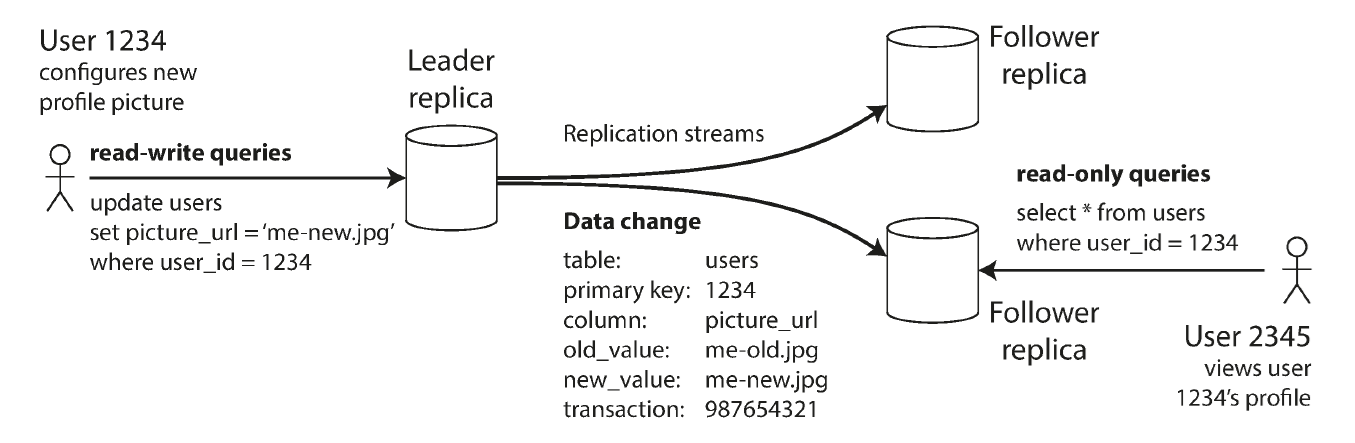
\includegraphics[width=0.8\textwidth]{resources/chapter-2/leader-based-replication.png}
    \caption{\textit{Leader-based (master-slave) replication \parencite{dataIntensiveApplications}}}
    \label{fig:leader-based-replication}
\end{figure}

Selain itu, proses replikasi juga terbagi menjadi dua, yaitu \textit{synchronous replication} dan \textit{asynchronous replication}. Pada \textit{synchronous replication}, data yang akan ditulis juga harus sudah ditulis oleh semua (atau mayoritas) replika sebelum dapat di-\textit{acknowledge}. Pada \textit{asynchronous replication}, data akan ditulis terlebih dahulu pada \textit{leader} lalu perubahannya dipropagasikan kepada \textit{replika}. Setiap pendekatan ini memiliki \textit{tradeoff} tersendiri. \textit{Synchronous replication} menjamin mayoritas \textit{node} memiliki data paling terbaru, tetapi latensi pada proses penulisan akan meningkat, sedangkan pada \textit{asynchronous replication} latensi penulisan jauh lebih kecil, tetapi data pada \textit{replica} menjadi \textit{eventually consistent}. Kedua mode replikasi ini didukung oleh PostgreSQL.

\section{\textit{Event-Driven Architecture}}

\textit{Event-driven architecture} merupakan paradigma arsitektur perangkat lunak yang berkaitan dengan produksi dan deteksi \textit{event}. Arsitektur ini mudah dievolusikan dan menawarkan toleransi kegagalan (\textit{fault tolerance}), kinerja yang baik, dan pemskalaan yang baik. Meskipun begitu, arsitektur ini kompleks dan sulit untuk diuji. Arsitektur ini cocok untuk kasus yang kompleks dan dinamis \parencite{softwareArchitecture}.

Arsitektur ini terdiri atas tiga komponen, yaitu \textit{event producer}, \textit{event router}, dan \textit{event consumer}. Sebuah produsen mengirimkan \textit{event} ke \textit{router}, lalu disaring dan dikirimkan kepada konsumen.

\subsection{Redpanda}

Redpanda merupakan \textit{event streaming platform}. Platform ini menyediakan infrastruktur untuk \textit{streaming real-time data}. Produsen mengirimkan data berupa \textit{event} ke Redpanda, kemudian Redpanda menyimpan \textit{event} tersebut lalu mengaturnya ke dalam sebuah topik. Topik ini merupakan log \textit{event} yang dapat diputar ulang. Konsumen mengonsumsi \textit{event} pada topik Redpanda secara asinkron \parencite{redpandaIntro}.

\begin{figure}[htbp]
    \centering
    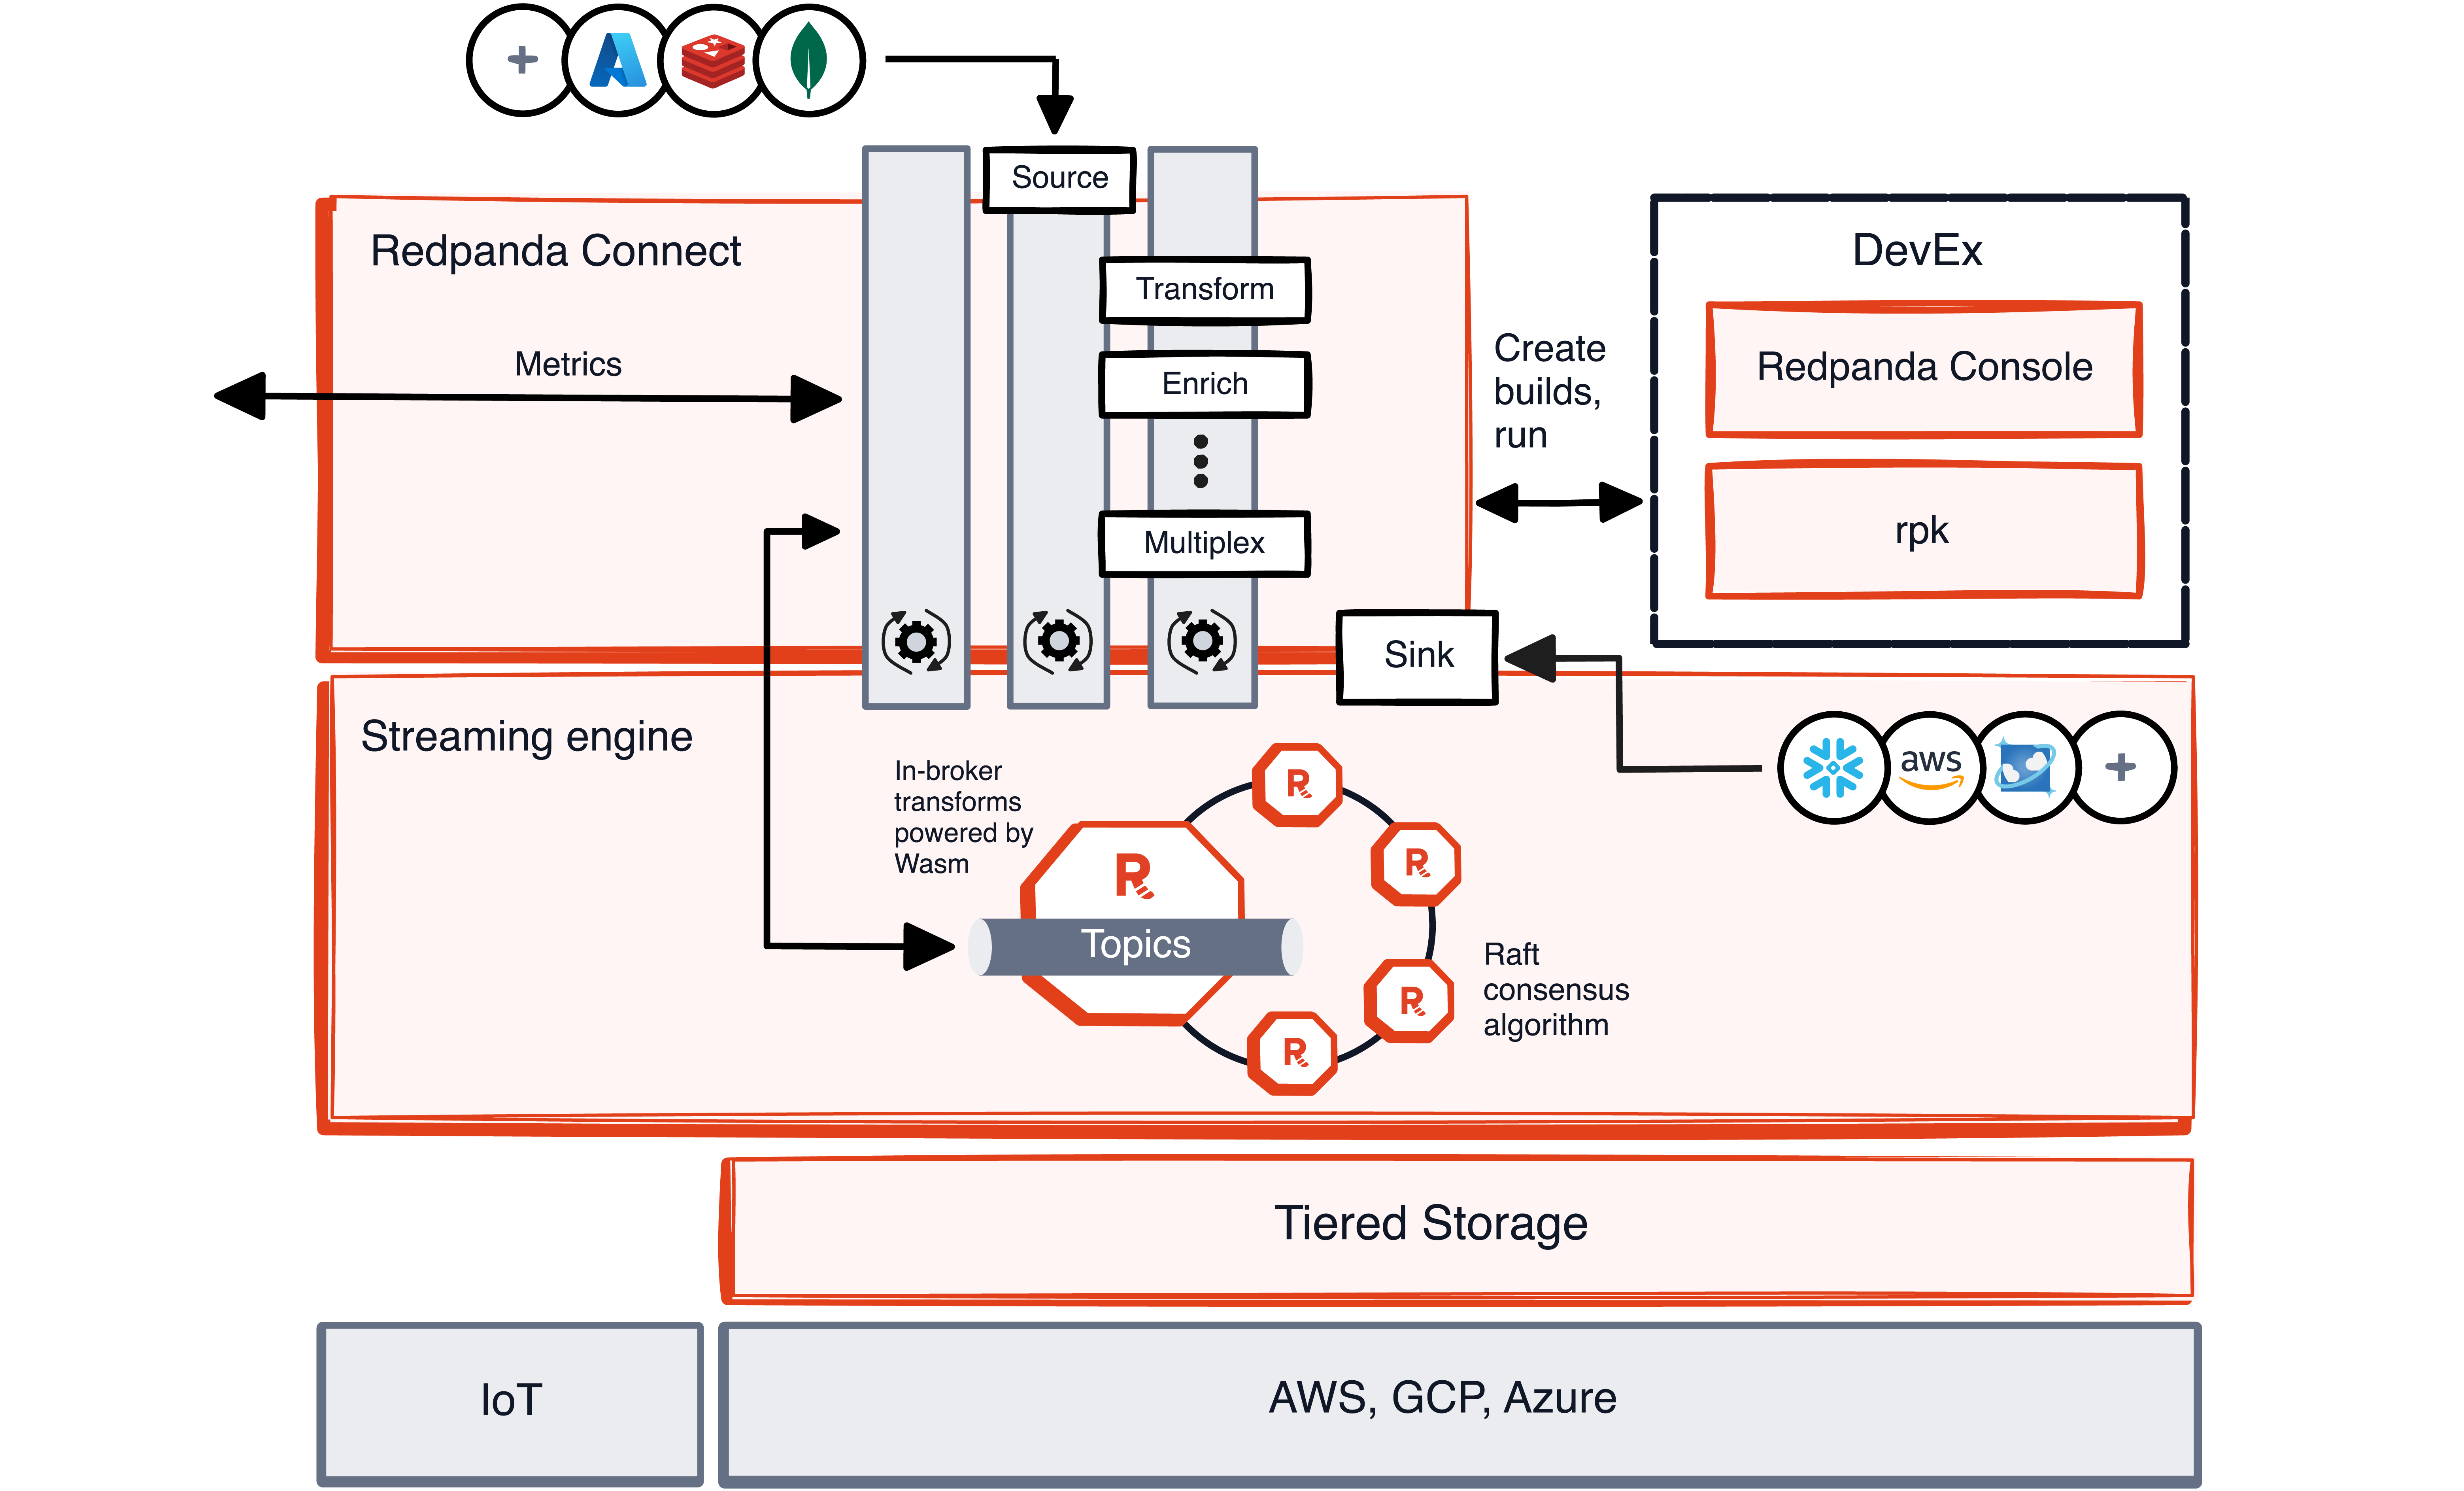
\includegraphics[width=0.8\textwidth]{resources/chapter-2/redpanda.png}
    \caption{Apa itu Redpanda? \parencite{whatIsRedpanda}}
    \label{fig:what-is-redpanda}
\end{figure}

Redpanda merupakan \textit{event streaming platform} alternatif dari Apache Kafka. Selain itu, platform ini menawarkan kompatibilitas API yang sama dengan Kafka sehingga memudahkan migrasi penggunanya. Meskipun begitu, terdapat beberapa perbedaan antara Redpanda dengan Apache Kafka.

Perbedaan pertama adalah algoritma konsensus yang digunakan. Apache Kafka menggunakan ZooKeeper (versi lama) sedangkan Redpanda menggunakan Raft. Meskipun begitu, versi terbaru Kafka sudah menggunakan algoritma konsensus Kraft yang merupakan varian dari Raft dengan perbedaan pada mekanisme replikasi log \parencite{raftKraft}.

Selain itu, Redpanda berfokus pada pengoptimalan kinerja yang lebih baik dibandingkan dengan Apache Kafka. Redpanda ditulis dalam bahasa C++, sedangkan Apache Kafka ditulis dalam bahasa Java dan berjalan pada JVM. Dalam hal ini, Redpanda menggunakan bahasa sistem sehingga minim \textit{overhead}.

Berikut adalah contoh pengoptimalan yang dilakukan pada Redpanda: \textit{Direct Memory Access (DMA)} untuk I/O, distribusi pemrosesan \textit{interrupt request} (IRQ) pada beberapa core CPU, penggunaan model \textit{thread per core}, dan pengoptimalan lainnya. Penggunaan model \textit{thread per core} memungkinkan Redpanda untuk menjalankan \textit{thread} aplikasi pada inti CPU yang sama sehingga \textit{context switching} dan \textit{blocking} dapat dihindari \parencite{redpandaArchitecture}.

\subsection{\textit{Change Data Capture}}

Menurut \cite{dataIntensiveApplications}, \textit{change data capture (CDC)} merupakan sebuah proses yang mengobservasi setiap perubahan pada data yang ditulis ke dalam basis data dan mengekstraknya ke dalam bentuk yang bisa direplikasi oleh sistem lain. Sebagai contoh, perubahan pada database bisa di-\textit{capture} lalu diterapkan pada \textit{search index} untuk menyamakan data pada basis data. Apabila \textit{log} diaplikasikan dalam urutan yang sama, data pada \textit{search index} dan basis data bisa dipastikan sama.

\begin{figure}[ht]
    \centering
    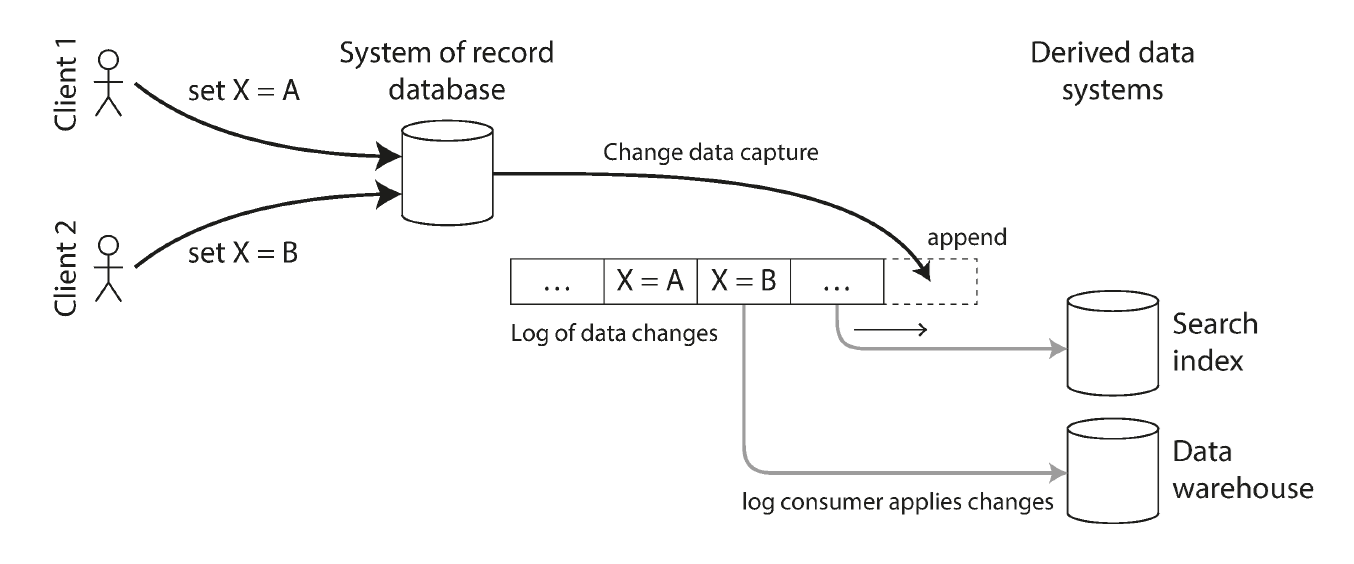
\includegraphics[width=0.8\textwidth]{resources/chapter-2/cdc.png}
    \caption{\textit{CDC Illustration \parencite{dataIntensiveApplications}}}
    \label{fig:cdc-illustration}
\end{figure}

PostgreSQL juga mendukung CDC dengan istilah \textit{logical replication}. Mekanisme ini menggunakan model \textit{publish} dan \textit{subscribe}. PostgreSQL yang mengirimkan \textit{log} bertindak sebagai \textit{publisher}, lalu terdapat \textit{subscriber} lain yang mengonsumsi \textit{log} yang dipublikasikan. \textit{Subscriber} ini bisa berupa replika PostgreSQL lagi atau aplikasi lainnya \parencite{pgLogicalReplication}. PostgreSQL mendukung dua mode operasi untuk replikasi, yaitu replikasi secara \textit{asynchronous} dan \textit{synchronous} \parencite{insideLogicalReplication}. Pada mode \textit{synchronous}, \textit{subscriber} harus merespons terlebih dahulu terhadap perubahan data sebelum PostgreSQL dapat melakukan \textit{commit}.

\begin{figure}[ht]
    \centering
    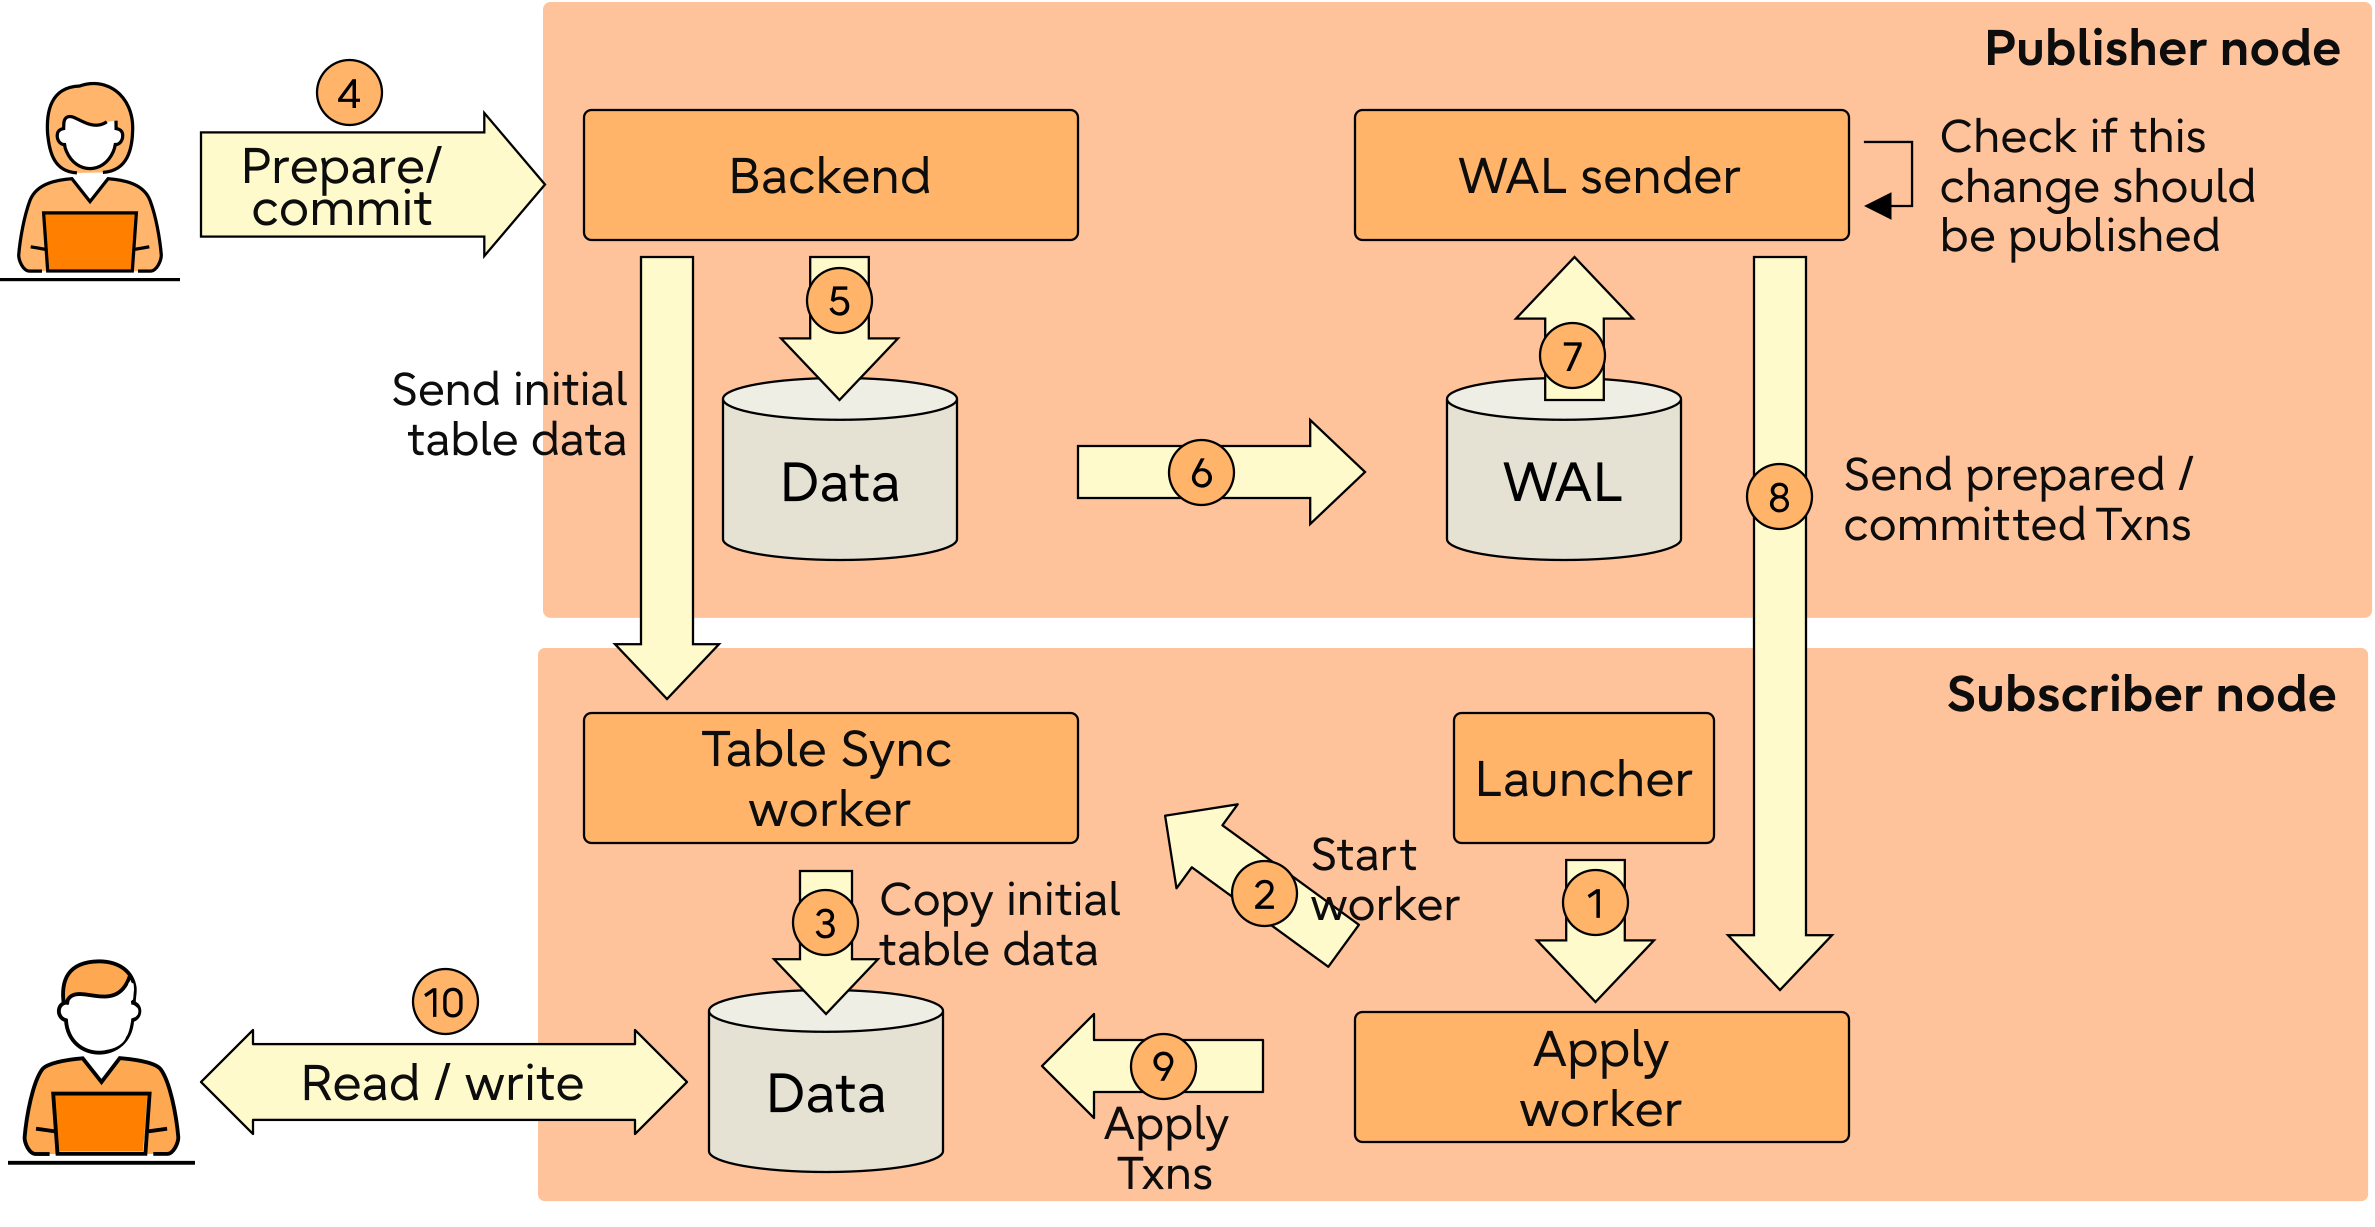
\includegraphics[width=0.8\textwidth]{resources/chapter-2/postgres-logical-replication.png}
    \caption{\textit{Logical Replication Architecture \parencite{insideLogicalReplication}}}
    \label{fig:logical-replication-architecture}
\end{figure}



\subsection{\textit{Event Sourcing}}

Mirip seperti \textit{change data capture}, \textit{event sourcing} juga menyimpan setiap perubahan pada \textit{state} aplikasi sebagai \textit{log of events}. Perbedaan terbesarnya terletak pada level abstraksinya. Pada \textit{change data capture}, aplikasi menggunakan basis data \textit{in a mutable way} dan dapat memperbarui atau menghapus \textit{record} sesuka hati. Aplikasi yang menulis pada basis data tidak harus \textit{aware} bahwa terdapat CDC. Berbeda dengan \textit{event sourcing}, logika aplikasi dibandung secara eksplisit di atas asumsi \textit{immutable event} yang ditulis pada \textit{event log}. Pada kasus ini, \textit{event} berupa \textit{append only}. Singkatnya, \textit{event sourcing} didesain untuk bisa merefleksikan hal yang terjadi pada level aplikasi dan bukan pada \textit{low-level state changes}.

\section{Pemrosesan \textit{Stream}}

Secara umum, \textit{stream} merujuk pada data yang tersedia secara inkremental dari waktu ke waktu. Konsep ini dipakai di berbagai tempat, seperti stdin dan stdout Unix, koneksi TCP, dan lain-lain \parencite{dataIntensiveApplications}.

\textit{Stream processing} merupakan paradigma pemrograman yang memandang \textit{stream} atau urutan \textit{event} sebagai objek masukan dan luaran utama dari komputasi. \cite{streaming101} menyatakan bahwa \textit{stream processing} merupakan tipe mersin pemrosesan data yang didesain dengan mempertimbangkan data yang tidak terbatas.

\cite{streamProcessingComparison} menyatakan bahwa terdapat karakteristik penting pada \textit{stream processing}, yaitu:

\begin{enumerate}
    \item \textit{Delivery guarantees}. Setiap informasi yang masuk harus dijamin akan diproses oleh \textit{streaming engine}.
    \item Toleransi kegagalan (\textit{fault tolerance}). Ketika terjadi kegagalan, \textit{streaming engine} harus mampu melakukan pemulihan dan memulai ulang dari titik yang ditinggalkan.
    \item \textit{State management}. \textit{Streaming engine} harus memiliki mekanisme untuk menyimpan dan memperbarui informasi \textit{state}.
    \item Memiliki kinerja yang baik dari sisi latensi, \textit{throughput}, dan skalabilitas.
    \item Memiliki fitur yang lebih canggih, seperti \textit{event time processing}, \textit{watermarks}, \textit{windowing}, dan lain-lain.
\end{enumerate}

Selain itu, karakteristik \textit{stream processing} juga bisa dibagi menjadi dua jenis, yaitu:

\begin{enumerate}
    \item \textit{Native streaming}. \textit{Stream processing} jenis ini akan langsung memproses data yang diterima secepat mungkin. Contoh \textit{stream processing} tipe ini adalah Apache Storm, Apache Flink, Apache Kafka Streams, dan Apache Samza.
    \item \textit{Micro-batching}. \textit{Stream processing} jenis ini meproses data setiap beberapa detik atau milidetik sekali sehingga data diproses dalam setiap kelompok kecil dengan sedikit keterlambatan. Contoh \textit{stream processing} tipe ini adalah Apahe Spark Streaming dan Apache Storm-Trident.
\end{enumerate}

\subsection{RisingWave}

RisingWave merupakan \textit{cloud-native streaming database}. Setelah menghubungkan sumber \textit{stream}, pengguna dapat membuat kueri analisis dengan mendefinisikan \textit{materialized view}, yang diperbarui secara inkremental pada RisingWave \textit{streaming engine} \parencite{risingwave}.

Berikut adalah keuntungan RisingWave:

\begin{enumerate}
    \item Mudah dipelajari karena merupakan ekstensi dari sintaks PostgreSQL.
    \item Mudah dioperasikan dan memiliki kebutuhan sumber daya yang lebih rendah karena ditulis dalam bahasa sistem Rust.
    \item Mendukung berbagai sumber data dan mampu mengirimkan (\textit{sink}) data ke dalam berbagai sumber, seperti mengambil data dari Apache Kafka lalu hasilnya dikirim ke ClickHouse. RisingWave mendukung integrasi dengan PostgreSQL CDC dan Apache Kafka sebagai sumber (\textit{source}) dan tujuan data (\textit{sink}).
    \item Menjamin konsistensi pada \textit{materialized view} dengan menggunakan \textit{snapshot}.
\end{enumerate}

\begin{figure}[ht]
    \centering
    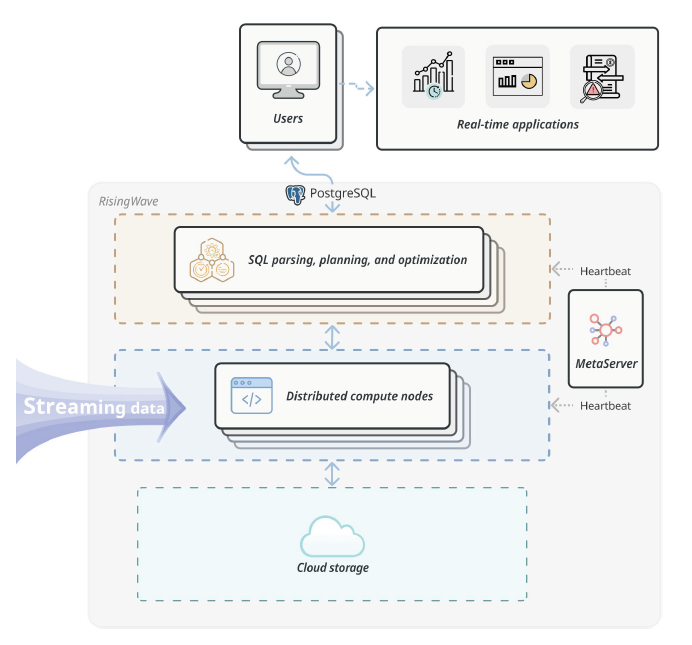
\includegraphics[width=0.8\textwidth]{resources/chapter-2/risingwave.png}
    \caption{Arsitektur RisingWave \parencite{risingwave}}
    \label{fig:risingwave-architecture}
\end{figure}

Node komputasi pada RisingWave terdiri atas \textit{batch engine} dan \textit{streaming engine}. \textit{Batch engine} meliputi \textit{query execution engine} dan \textit{exchange service} untuk menukar data antar node komputasi. \textit{Streaming engine} dibangun atas model aktor pada pemrograman konkuren. Mesin ini berinteraksi langsung dengan \textit{frontend} dan melayani \textit{stream data}. Selain itu, terdapat \textit{meta service} yang berperan sebagai layanan sentral untuk menyimpan metadata seperti keadaan kluster, katalog sistem, keanggotaan kluster, dan lain-lain \parencite{risingwave}.

\section{Pola Penyeimbangan Beban Berbasiskan Antrean}

Sebuah layanan dalam satu sistem seringkali bertugas untuk mengerjakan sesuatu dan memanggil layanan lain. Dalam kasus ini, terdapat kemungkinan munculnya masalah kinerja dan keandalan ketika layanan mengalami beban yang tinggi. Keadaan ini dapat menciptakan situasi \textit{backpressure}.

Dalam konteks perangkat lunak, \textit{backpressure} dapat didefinisikan sebagai \textit{resistance or force opposing the desired flow of data through software} \parencite{backpressureExplained}. Selain melakukan penyesuaian pada sumber daya sistem, terdapat tiga strategi yang dapat digunakan untuk menangani \textit{backpressure}, yaitu:

\begin{enumerate}
    \item Mengurangi kecepatan produsen mengirimkan pesan.
    \item Menggunakan \textit{buffer} untuk sementara mengakumulasikan pesan.
    \item Membuang (\textit{drop}) sebagian pesan yang diterima.
\end{enumerate}

Pola penyeimbangan beban berdasiskan antrean (\textit{Queue-based load leveling}) merupakan pola desain yang menyelesaikan masalah \textit{backpressure} dengan menggunakan antrean yang bertindak sebagai \textit{buffer} antara pesan dengan sebuah layanan, sehingga beban dapat dikontrol dan layanan tetap berjalan dengan stabil \parencite{queueLoadLeveling}.

\begin{figure}[ht]
    \centering
    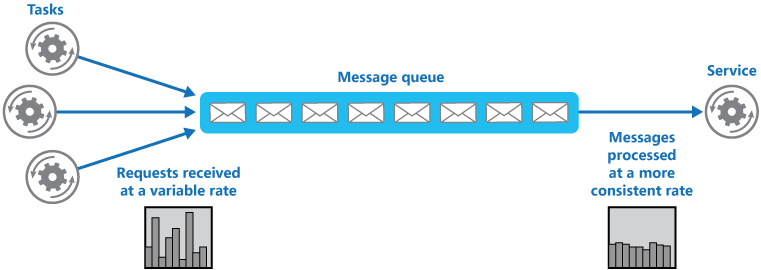
\includegraphics[width=0.8\textwidth]{resources/chapter-2/queue-based-load-leveling-pattern.png}
    \caption{Contoh Pola Penyeimbangan Beban Berbasiskan Antrean \parencite{queueLoadLeveling}}
    \label{fig:queue-based-load-leveling-pattern}
\end{figure}

Penggunaan antrean memisahkan pesan dengan pekerja, sehingga pekerja dapat menangani pesan berdasarkan kemampuannya, terlepas dari banyaknya pekerjaan yang bertambah seiring dengan berjalannya waktu. Pola ini memiliki berbagai keuntungan, seperti menjaga ketersediaan, memaksimalkan skalabilitas, dan membatasi biaya atau penggunaan sumber daya. Meskipun begitu, penggunaan pola ini akan meningkatkan latensi, terlebih lagi apabila pesan yang dikirimkan jauh lebih besar daripada kapasitas pemrosesan pada sistem.
% \blankpage
% \chapter{Analisis Masalah dan Rancangan Solusi}

\chapter{Analisis Sistem}

\section{Komponen Sistem Tiket}

Berdasarkan studi yang sudah dibahas sebelumnya dan berdasarkan fokus yang ingin dibahas pada penelitian ini, berikut adalah komponen sistem yang menjadi bahasan dari penelitian ini:

\begin{enumerate}
    \item Layanan \textit{backend} utama yang memproses setiap permintaan yang berkaitan dengan pemesanan tiket.
    \item Layanan otentikasi.
    \item Layanan gerbang pembayaran. Layanan ini merupakan layanan eksternal dan cukup melakukan \textit{mocking service}.
    \item Terdapat satu basis data utama sebagai sumber kebenaran utama.
\end{enumerate}

Daftar acara dan ketersediaan awal tiket merupakan data yang diisi dari awal, sehingga fitur manajemen acara dan tiket tidak diimplementasikan. Detail lengkap komponen dan fitur sistem dijelaskan pada bagian lampiran.



\section{Analisis Masalah}

Penjualan tiket acara dengan tingkat peminat serupa dengan penjualan tiket Taylor Swift dan Coldplay tentu akan terjadi lagi di masa mendatang. Meskipun begitu, tidak semua penyedia layanan terbiasa menangani beban pada skala ini. Kebanyakan penyedia layanan menggunakan solusi antrean virtual yang membatasi jumlah pengguna yang mengakses situs secara bersamaan. Pendekatan ini memang membantu meringankan beban sistem dan menjaga stabilitas. Meskipun begitu, banyak pengguna yang harus menunggu lama untuk bisa mengakses platform.

Di sisi lain, belum banyak studi yang membahas skalabilitas sistem dengan kasus seperti ini. \cite{microservicesEventDriven} membahas desain arsitektur yang \textit{fault-tolerant} dan tidak membahas aspek skalabilitas. \cite{backendForTicketing} juga tidak membahas arsitektur sistem dari sisi skalabilitas. Berdasarkan pertimbangan di atas, diperlukan desain arsitektur yang optimal dan mampu menangani beban seperti ini. Solusi ini tidak serta merta mengganti solusi antrean virtual. Dengan adanya arsitektur yang optimal, jumlah pengguna yang bisa dilayani dalam satu waktu dapat meningkat dan proses penjualan menjadi lebih cepat tanpa kendala.

Beban sistem tiket dapat dibagi menjadi dua: pemrosesan pemesanan tiket dan permintaan baca ketersediaan tiket. Pada kasus tiket, akan ada banyak pengguna yang ingin memesan tiket secara bersamaan. Oleh karena itu, \textit{raw throughput} yang dapat diberikan oleh basis data harus ditingkatkan. Basis data relasional saat ini memang memungkinkan \textit{scaling out} dengan menambah jumlah instans, tetapi instans yang dapat menulis data tetap ada satu sehingga batas \textit{write throughput} hanya dapat ditingkatkan dengan melakukan penskalaan vertikal. Di sisi lain, basis data relasional terus berkembang dan sudah ada berbagai solusi yang memungkinkan basis data relasional mendukung \textit{multiple-writer}. Peningkatan penskalaan ini memungkinkan peningkatan jumlah pengguna yang dapat dilayani dalam satu waktu.

Pada saat yang bersamaan, terjadi \textit{write contention} saat pemesanan tiket. Skema \textit{locking} diperlukan agar tidak terjadi \textit{double-booking} dan skema pengendalian aliran juga diperlukan agar percobaan pemesanan tiket dapat berkurang/ ditolak lebih cepat sebelum masuk ke basis data. Selain itu, skema ini juga memungkinkan tercapainya stabilitas sistem yang lebih baik.


\section{Analisis Solusi}

\subsection{Pencegahan \textit{Double Booking}}

Penggunaan basis data relasional seperti PostgreSQL memungkinkan implementasi pemesanan tiket yang lebih mudah dan terjamin konsistensinya. Untuk mencegah \textit{double booking}, basis data dapat melakukan \textit{row-level locking} di dalam transaksi, sehingga setiap \textit{seat} hanya terjual sebanyak satu kali.

\subsection{Peningkatan \textit{Raw Throughput} Pemesanan Tiket}

Penskalaan \textit{throughpupt} penulisan pada basis data relasional tradisional seperti PostgreSQL terbatas pada maksimal CPU, Memori, dan \textit{throughput} media penyimpanan yang dapat digunakan oleh suatu komputer. Penskalaan ini memiliki batas dari sisi teknologi dan peningkatan biayanya tidak sebanding dengan peningkatan kinerja yang dihasilkan. Oleh karena itu, skema PostgreSQL dengan \textit{primary} dan \textit{replica} memiliki keterbatasan dari sisi penulisan.

Penggunaan basis data nonrelasional berbasikan dokumen seperti MongoDB memang menarik karena menawarkan \textit{throughput} yang jauh lebih baik. Meskipun begitu, basis data tersebut tidak memiliki dukungan kueri transaksional sebagaimana yang dimiliki pada basis data relasional. Hal yang sama juga terjadi dengan penggunaan basis data berbasiskan \textit{wide-column}. Ide yang menyatakan bahwa basis data relasional tidak \textit{scalable} perlu dipertanyakan karena keduanya memiliki pemodelan entitas yang jauh berbeda. Oleh karena itu, penelitian ini akan mengeksporasi basis data relasional yang dapat di-\textit{scale-out} sehingga \textit{write throughput} dapat meningkat.

Terdapat berbagai alternatif basis data relasional yang merupakan pengembangan dari basis data tradisional. PostgreSQL dan MySQL merupakan basis data relasional yang sudah umum diketahui. Di sisi lain, terdapat CitusData yang merupakan ekstensi PostgreSQL dan memungkinkan PostgreSQL mendukung \textit{multiple-writer} dengan skema \textit{sharding} baik dari sisi skema atau pun data \parencite{citus}. Hal yang sama juga terjadi pada ekosistem MySQL dengan Vitess \textit{Vitess}. Selain itu, terdapat basis data yang bukan merupakan pengembangan dari basis data yang ada seperti PostgreSQL dan MySQL dan merupakan pengembangan basis data yang dimulai dari nol dengan penggunaan konsensus seperti Raft dan protokol \textit{low-level} seperti RocksDB atau LevelDB. Meskipun begitu, basis data seperti itu tetap mengimplementasikan antarmuka yang sama pada PostgreSQL dan MySQL. CockroachDB merupakan basis data jenis ini yang kompatibel dengan antarmuka MySQL \parencite{cockroachDB}. YugaByteDB merupakan basis data jenis ini yang kompatible dengan antarmuka PostgreSQL \parencite{yugabyte}. Penggunaan basis data tersebut menarik untuk diuji kinerjanya dibandingkan dengan basis data biasa dan menarik untuk diketahui apakah penggunaan teknologi tersebut dapat membantu kinerja sistem tiket yang dibahas pada penelitian ini.

Dari sekian banyak alternatif basis data relasional, perlu dipilih basis data yang masing-masing dapat merepresentasikan pendekatan yang dipakai pada basis data tersebut. Basis data yang mendukung antarmuka PostgreSQL dipilih karena keakraban dengan teknologi tersebut. Selain itu, pemilihan basis data dengan antarmuka yang sama memungkinkan pengembangan yang lebih mudah dan perbandingan kinerja yang lebih adil. Oleh karena itu, PostgreSQL dipilih sebagai basis data yang menjadi dasar acuan, CitusData dipilih sebagai basis data yang mengembangkan PostgreSQL, sedangkan YugaByteDB dipilih sebagai basis data dengan ide berbeda, tetapi tetap mengimplementasikan antarmuka PostgreSQL.

\subsection{Penggunaan Skema \textit{Flow Control} Pada Pemesanan Tiket}

Dengan banyaknya pengguna yang ingin memesan tiket pada satu waktu, kemungkinan terjadinya \textit{write contention} sangat tinggi. Bila tidak ditangani dengan baik, kesalahan seperti \textit{double booking} dapat terjadi. Selain itu, basis data akan cukup sibuk menangani transaksi gagal dan menangani konflik selama proses kueri transaksional. Sebagaimana dibahas sebelumnya, penggunaan \textit{flow control} menarik untuk dieksplorasi lebih lanjut pengaruhnya terhadap kinerja sistem tiket. Setidaknya terdapat dua strategi \textit{flow control} yang dapat digunakan pada operasi pemesanan tiket, yaitu penggunaan \textit{buffer} atau antrian dan \textit{drop request}. Tentunya proses \textit{drop request} harus dilakukan secara strategis agar dapat mengurangi \textit{contention} tanpa menghalangi pembelian tiket yang masih tersedia. Ide dasar yang dapat digunakan adalah dengan membuang permintaan terhadap kursi yang sudah terjual atau akan terjual (terdapat \textit{request} lain yang memesan kursi yang sama, tetapi belum \textit{commited} atau pesanannya masih diproses oleh sistem). Proses \textit{filter} ini dapat dilimpahkan pada basis data yang memiliki latensi rendah seperti Redis. Meskipun begitu, tantangan pendekatan ini berada pada bagaimana cara memastikan data ketersediaan pada basis data dengan data ketersediaan pada Redis tetap tersinkronisasi terutama saat banyak terjadi kegagalan pada sistem.

Hal yang harus diperhatikan dari penggunaan Redis adalah aspek \textit{persistence}. Redis memiliki dua jenis \textit{persistence}, yaitu \textit{snapshot} dan \textit{Append-Only File}. Tentunya pada kasus ini \textit{persistence} penting untuk memitigasi kegagalan. Pengaturan yang paling direkomendasikan adalah penggunaan \textit{snapshot} dengan \textit{append-only file} (AOF). Pengaturan AOF sendiri memiliki dua pengaturan, yaitu \textit{everysec} dan \textit{always}. Opsi \textit{everysec} dipilih karena merupakan pengaturan yang menyeimbangkan kinerja dengan \textit{persistence}. Sekalipun terjadi kegagalan, data yang terdapat pada Redis dapat dibuat ulang dan permintaan yang tidak dapat ditolak pada tahap ini tetap akan ditolak pada tahap berikutnya.

Selain itu, penggunaan \textit{queue} didasari pada ide bahwa basis data akan kesulitan menangani banyak \textit{concurrent request}. Banyaknya \textit{request} yang menumpuk mengakibatkan latensi yang tinggi dan seringkali basis data tidak dapat \textit{recover} dari kondisi tersebut kecuali bebannya dikurangi secara signifikan. Oleh karena itu, penting agar menjaga basis data pada utilisasi yang optimal sehingga basis data dapat beroperasi dengan baik. Oleh karena itu, proses pemrosesan pemesanan tiket seharusnya disesuaikan berdasarkan kapasitas basis data untuk menjaga stabilitas sistem.

Apakah itu berarti proses pemesanan tiket menjadi asinkron? belum tentu. Operasi ini tetap diimplementasikan secara sinkron yang berupa pemanggilan HTTP lalu meunggu respons dari server. Hanya saja, permintaan pengguna di-\textit{queue} terlebih dahulu. \textit{Tradeoff} dari implementasi ini adalah latensi yang lebih tinggi yang akan dirasakan dari sisi pengguna. Klasifikasi yang tepat adalah \textit{partial synchrony}. Sistem ini \textit{synchronous} pada sebagian besar waktu, tetapi dapat menjadi asinkron saat terjadi hal-hal yang tidak diinginkan.

Dengan pendekatan seperti itu muncul masalah terutama bagaimana menangani kegagalan atau permintaan yang melewati batas waktu tertentu. Untuk menangani hal tersebut, implementasi proses pemesanan tiket dapat dibuat idempoten dengan menyertakan \textit{idempotency key} sehingga apabila sebuah pemesanan tiket mengalami \textit{timeout} dari sisi klien, tetapi tetap diproses dengan sukses oleh server meski setelah beberapa waktu tertentu, proses pemesanan tetap dapat dilanjutkan sebagaimana mestinya tanpa harus membuat pesanan baru.

Konsiderasi berikutnya adalah pemiilhan broker \textit{message queue}. Dari sisi kinerja, penggunaan \textit{event-streaming platform} seperti Kafka atau Redpanda menawarkan latensi yang jauh lebih baik dengan penskalaan yang jauh lebih baik \parencite{comparingKafkaAlternatives}. meskipun begitu, \textit{overhead} implementasi untuk menjadikan \textit{platform} tersebut sebagai \textit{message queue platform} tradisional membutuhkan investasi yang tinggi, sehingga tidak dapat diimplementasikan dalam waktu yang singkat. Oleh karena itu, \textit{message queue platform} tradisional seperti RabbitMQ dipilih karena memiliki \textit{overhead} implementasi yang lebih rendah dan \textit{deployment} yang lebih mudah. Solusi ini merupakan solusi yang sudah terbukti dan memilki fitur yang lengkap. Selain itu, meskipun beban yang diterima sangat tinggi, pada akhirnya jumlah permintaan yang masuk untuk proses pemesanan tiket akan jauh lebih sedikit sehingga keterbatasan penskalaan pada RabbitMQ tidak akan menjadi masalah.

\subsection{Pengoptimalan Operasi Baca Ketersediaan Tiket}

Pada sistem referensi, terdapat dua operasi baca ketersediaan tiket, yaitu operasi baca ketersediaan berdasarkan area dan operasi baca ketersediaan kursi berdasarkan area.

Operasi pembacaan ketersediaan berdasarkan area merupakan operasi agregat terhadap data yang selalu diperbarui dan merupakan operasi yang paling banyak dipanggil mengikuti banyaknya pengguna yang ada. Keterbaruan data merupakan aspek penting, sehingga penggunaan \textit{cache} tidak serta merta dapat digunakan.

Penggunaan denormalisasi pada level basis data dapat digunakan, seperti menambahkan kolom sisa kursi tersedia. Meskipun begitu, pendekatan ini tidak dapat digunakan karena dapat menimbulkan \textit{contention} apabila sistem ingin meningkatkan \textit{throughput} penulisan sebanyak-banyaknya. Oleh karena itu, kolom hasil agregat ini tidak disimpan pada basis data, tetapi disimpan pada Redis yang dapat menangani hal ini dengan lebih baik. Sama seperti sebelumnya, tantangan pendekatan ini adalah bagaimana caranya memastikan data yang ada pada basis data dengan Redis tetap sinkron, terutama pada skenario yang memiliki banyak kegagalan.

Operasi berikutnya adalah operasi baca ketersediaan kursi berdasarkan area. Operasi ini membutuhkan data berdasarkan baris dan operasi ini memang lebih baik apabila langsung memanggil basis data. Meskipun begitu, pada \textit{traffic spike} yang tinggi dalam waktu singkat, operasi tersebut dapat membebani basis data. Dari sisi keterbaruan data, data yang 150 milisekon lebih lama tidak akan jauh berbeda dengan data paling terbaru. Terlebih lagi, sistem ini bukan sistem yang sangat sensitif sehingga perbedaan sekian milisekon akan mempengaruhi hasil secara signifikan. \textit{Tradeoff} kinerja yang ditawarkan dengan pendekatan ini membuat penggunaan \textit{micro-caching} jauh lebih bermanfaat untuk menjaga stabilitas sistem. Penyimpanan \textit{cache} dapat diimplementasikan dengan \textit{in-memory hashmap} untuk latensi yang lebih baik. TTL \textit{cache} sebesar 150 milisekon membuat penggunaan Redis tidak cocok karena perbedaan latensi yang bisa menjadi sangat signifikan.

\section{Rancangan Sistem Tiket}

\subsection{Komponen Sistem Tiket (tanpa Pengendalian Aliran)}

Komponen sistem tiket dapat dibagi menjadi beberapa bagian, yaitu layanan tiket, basis data relasional, dan kluster Redis. Komponen basis data relasional dapat dibagi menjadi tiga jenis, yaitu kluster PostgreSQL dengan replika baca, kluster CitusData, dan kluster YugabyteDB. Komponen ini yang akan menjadi sumber kebenaran utama dari sistem ini. Selain itu, kluster Redis digunakan untuk menyimpan data agregat ketersediaan berdasarkan area.

\begin{figure}[htbp]
    \centering
    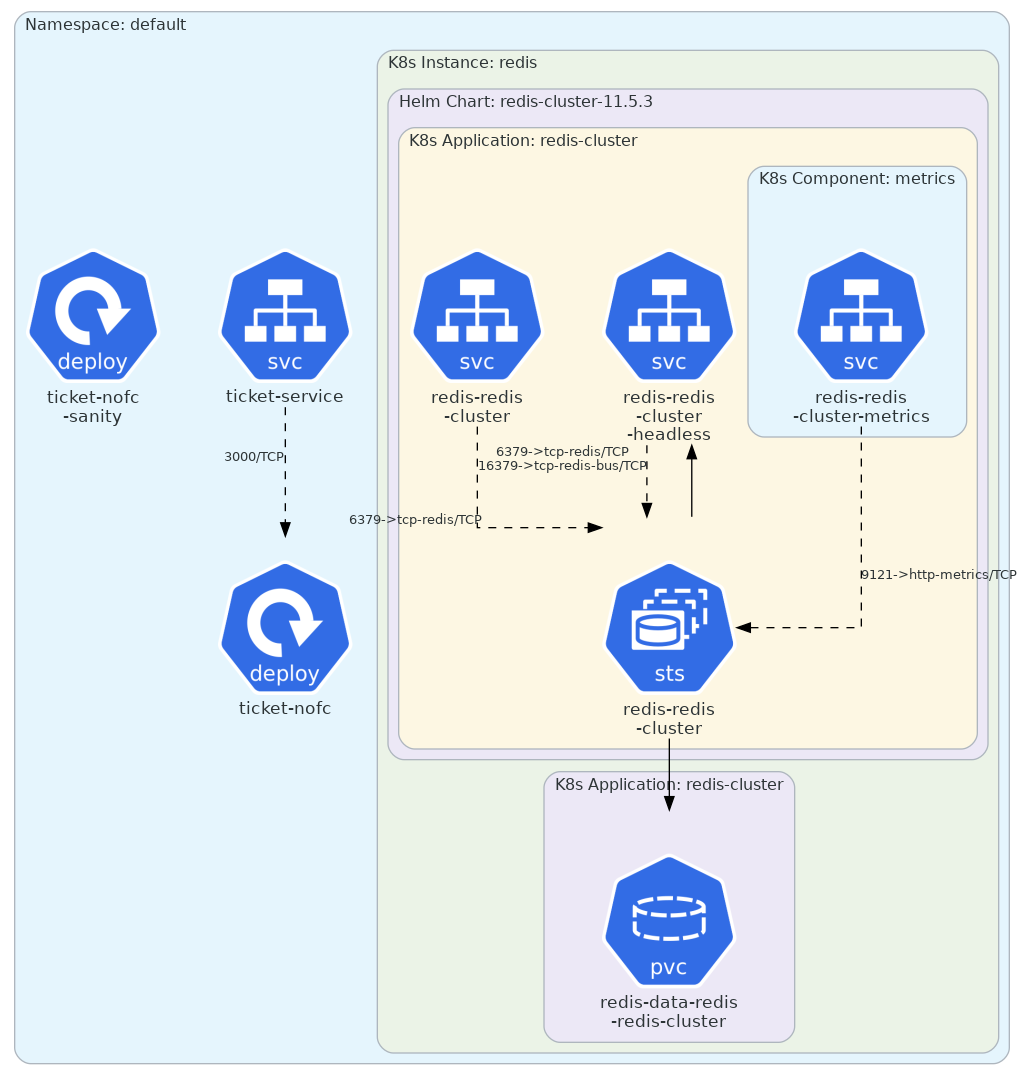
\includegraphics[width=0.8\textwidth]{resources/chapter-3/ticket-nofc.png}
    \caption{Diagram Arsitektur Sistem Tiket Tanpa Pengendalian Aliran}
    \label{fig:ticket-nofc}
\end{figure}

\pagebreak

\subsection{Komponen Sistem Tiket (dengan Pengendalian Aliran)}

\begin{figure}[htbp]
    \centering
    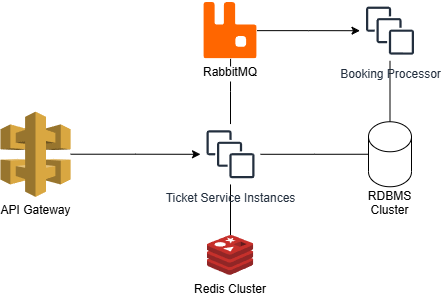
\includegraphics[width=0.8\textwidth]{resources/chapter-3/ticket-fc.png}
    \caption{Diagram Arsitektur Sistem Tiket dengan Pengendalian Aliran}
    \label{fig:ticket-fc}
\end{figure}

Pada sistem tiket dengan pengendalian aliran, terdapat dua komponen baru yaitu RabbitMQ dan pemroses pesanan. RabbitMQ bertugas untuk menyimpan antrean permintaan pemesanan tiket dan pemroses pesanan bertugas untuk memproses pemesanan tiket. Selain itu, kluster Redis memiliki tanggung jawab tambahan untuk menyimpan data yang digunakan untuk menolak permintaan pesanan yang masuk lebih awal.

\subsection{Variasi Basis Data Relasional}

Berikut adalah variasi konfigurasi basis data relasional yang mungkin terjadi.

\begin{figure}[htbp]
    \centering
    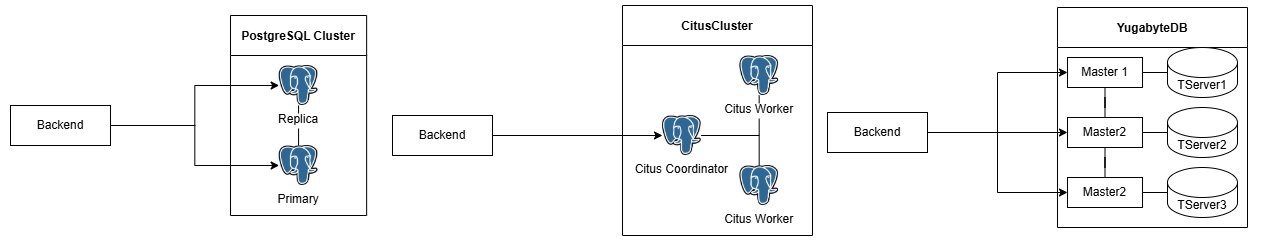
\includegraphics[width=1\textwidth]{resources/chapter-3/rdbms.png}
    \caption{Variasi Basis Data Relasional}
    \label{fig:rdbms-variation}
\end{figure}

Pada konfigurasi kluster PostgreSQL, klien terhubung dengan semua instans. Pada konfigurasi CitusData, klien hanya terhubung dengan koordinator dan koordinator yang akan meneruskan permintaan kepada \textit{worker}. Pada konfigurasi YugabyteDB, klien terhubung dengan semua Master yang masing-masing terhubung dengan TServer. Klien sebenarnya dapat terhubung dengan salah satu master saja, tetapi konfigurasi seperti ini membuat koneksi klien ke YugabyteDB menjadi lebih tahan terhadap kegagalan dan juga dapat mengurangi beban agar tidak terpusat pada satu instans saja.

Konfigurasi kluster PostgreSQL memiliki skalabilitas yang terbatas dengan peningkatan penulisan hanya dapat dicapai dengan penskalaan secara vertikal. Laju penulisan CitusData dan YugabyteDB dapat ditingkatkan dengan menambah jumlah instans.

\textit{Pooler} PGCat akan digunakan agar direct connection basis data yang terbatas dapat digunakan ulang dan dipakai oleh client yang lebih banyak. Selain itu, pada konfigurasi kluster PostgreSQL \textit{pooler} ini berguna sebagai pembagi beban kueri baca antara \textit{primary} dan replika.

\subsection{Alur Sistem Tiket}

\subsubsection{Alur Fitur Acara}

Terdapat tiga operasi pada fitur acara, yaitu membaca ketersediaan acara, membaca agregat ketersediaan area, dan membaca ketersediaan kursi. Operasi baca agregat ketersediaan area menggunakan data agregat yang dipelihara pada Redis alih-alih melakukan agregat dari basis data. Operasi baca ketersediaan kursi membaca langsung data dari basis data dengan sedikit pengoptimalan dengan menggunakan tembolok mikro.

\pagebreak

\begin{figure}[h]
    \centering
    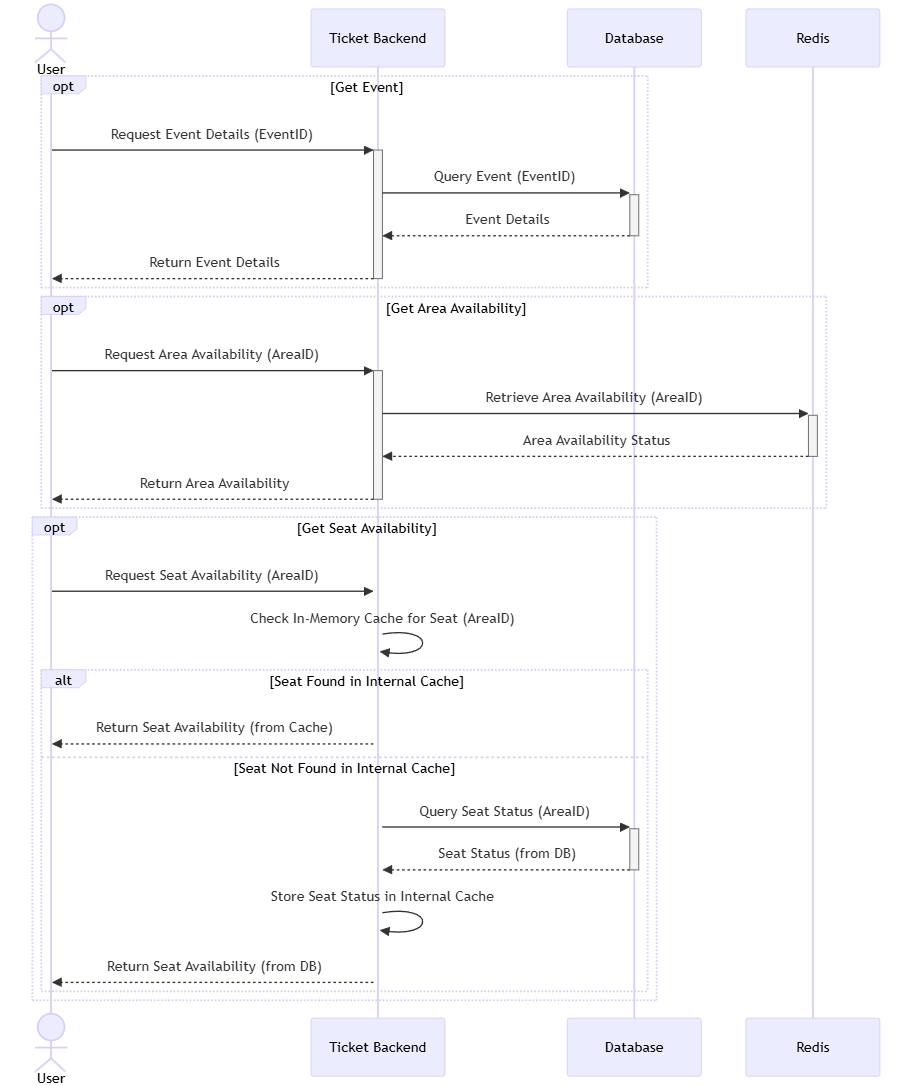
\includegraphics[width=1\textwidth]{resources/chapter-3/event-flow.png}
    \caption{Diagram Alur Fitur acara}
    \label{fig:flow-event}
\end{figure}

\pagebreak

\subsubsection{Alur Fitur Pemesanan Tiket (tanpa pengendalian aliran)}

Proses pemesanan tiket dimulai dengan pengguna mengirimkan permintaan pemesanan kepada sistem tiket.

\begin{figure}[htbp]
    \centering
    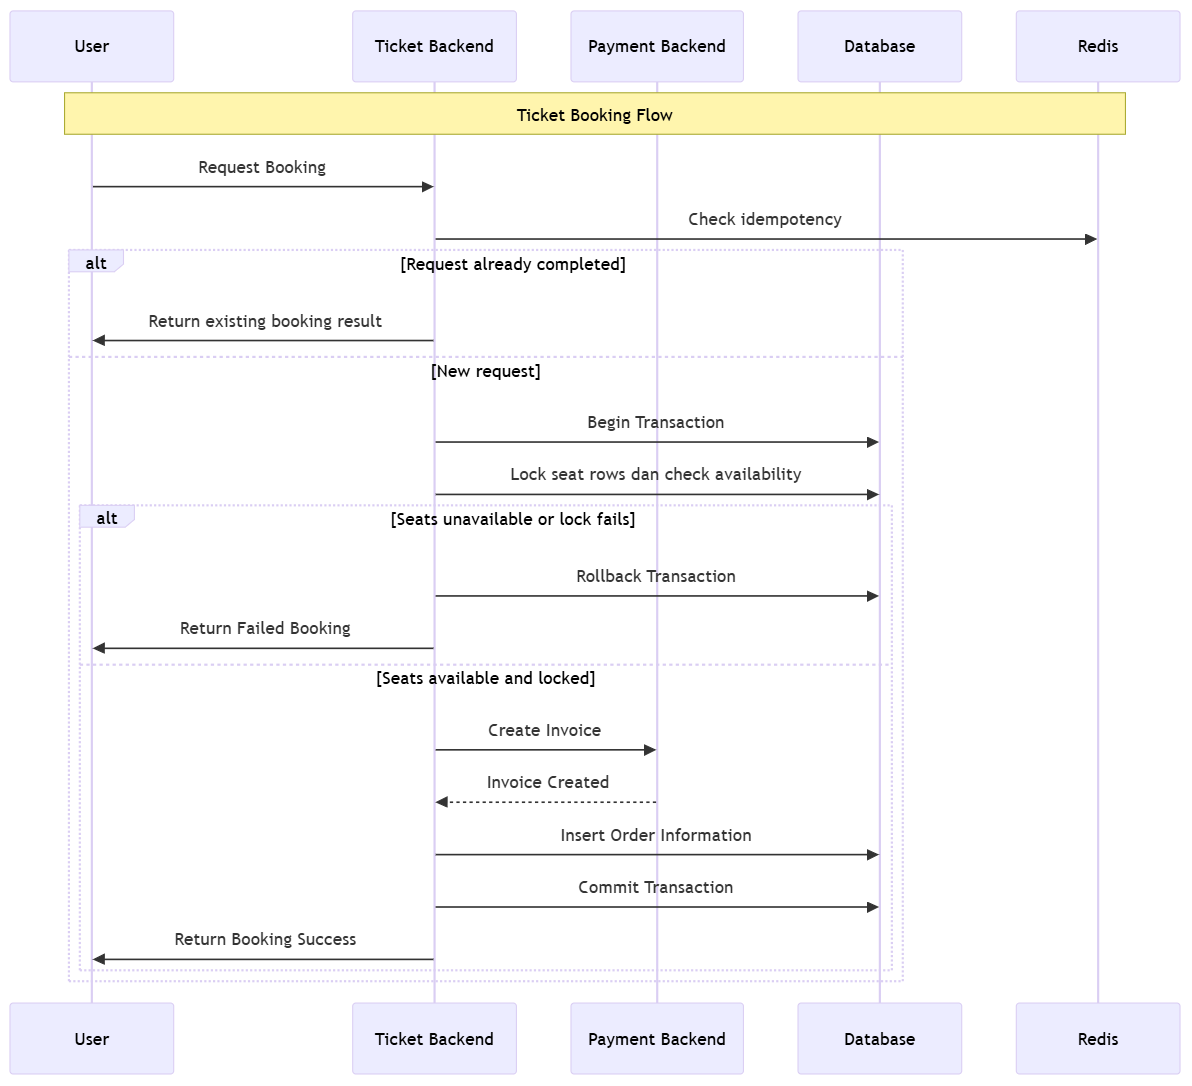
\includegraphics[width=1\textwidth]{resources/chapter-3/book-flow.png}
    \caption{Diagram Alur Fitur Pemesanan Tiket (tanpa pengendalian aliran)}
    \label{fig:flow-book-flow}
\end{figure}

\pagebreak

Ketika pengguna berhasil memesan, pengguna akan melakukan pembayaran kepada gerbang pembayaran. Setelah pembayaran selesai, pengguna memeriksa status pesanan yang telah dibuat.

\begin{figure}[h]
    \centering
    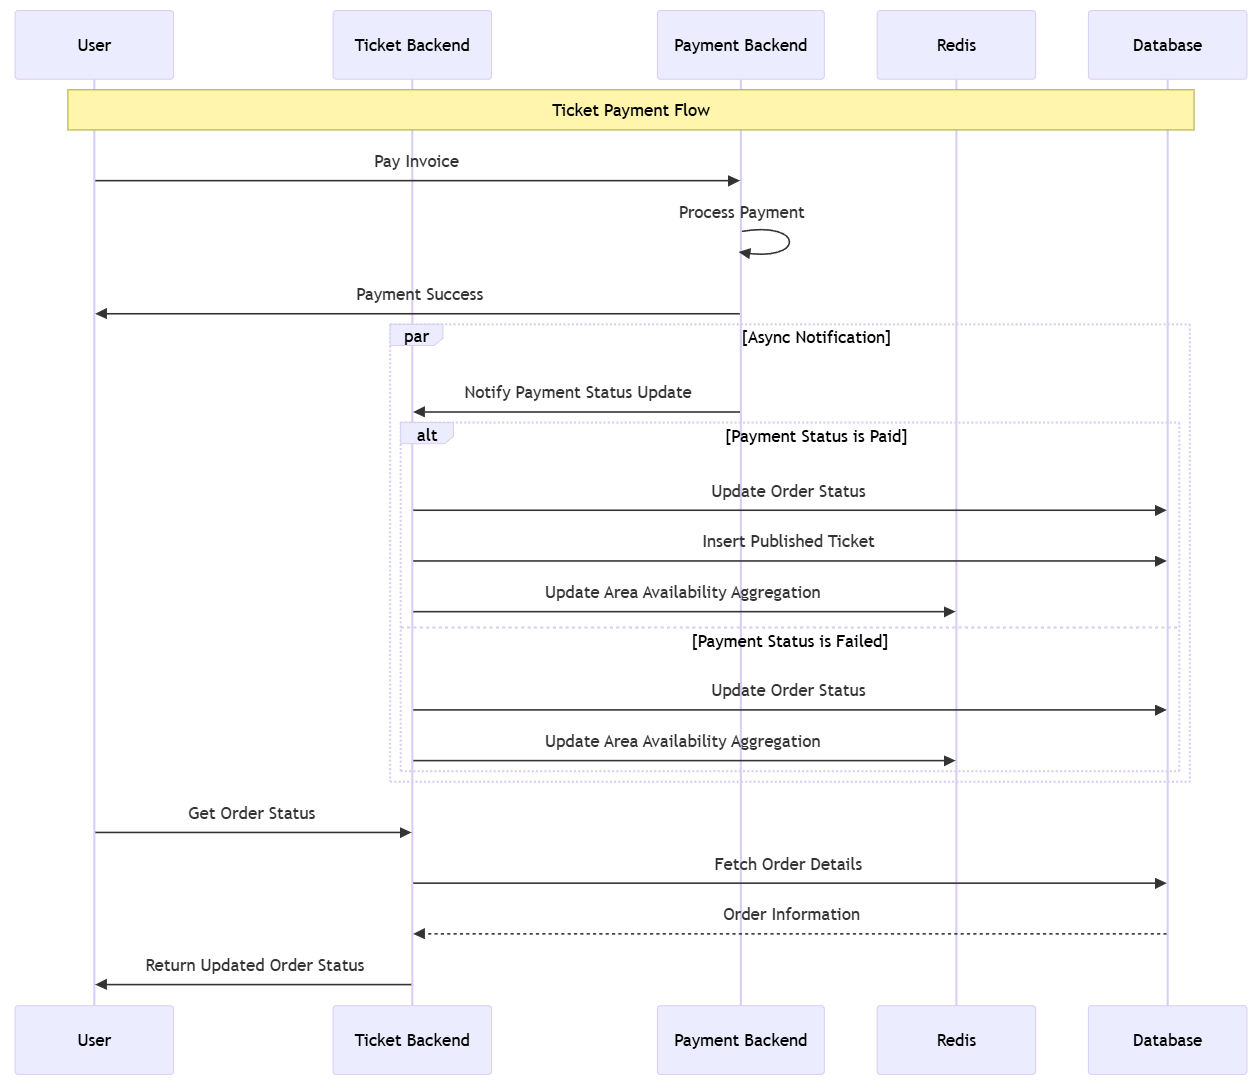
\includegraphics[width=1\textwidth]{resources/chapter-3/order-payment.png}
    \caption{Diagram Alur Fitur Pembayaran Tiket (tanpa pengendalian aliran)}
    \label{fig:flow-order-payment-flow}
\end{figure}

\pagebreak

\subsubsection{Alur Fitur Pemesanan Tiket (dengan pengendalian aliran)}

Proses pemesanan tiket dimulai dengan pengguna mengirimkan permintaan pemesanan kepada sistem tiket. Perbedaan dengan alur tanpa pengendalian aliran adalah penggunaan RabbitMQ dan pemroses pesanan. Proses pemesanan akan diproses secara \textit{partial synchrony} agar sistem dapat memproses pesanan sesuai dengan kapatiasnya. Selain itu, pendekatan ini juga memeriksa data dari Redis untuk menolak sebuah pesanan ketika terdapat pesanan yang sama untuk suatu kursi, tetapi memiliki pesanan lain yang sedang diproses dan belum sepenuhnya berhasil.

\begin{figure}[h]
    \centering
    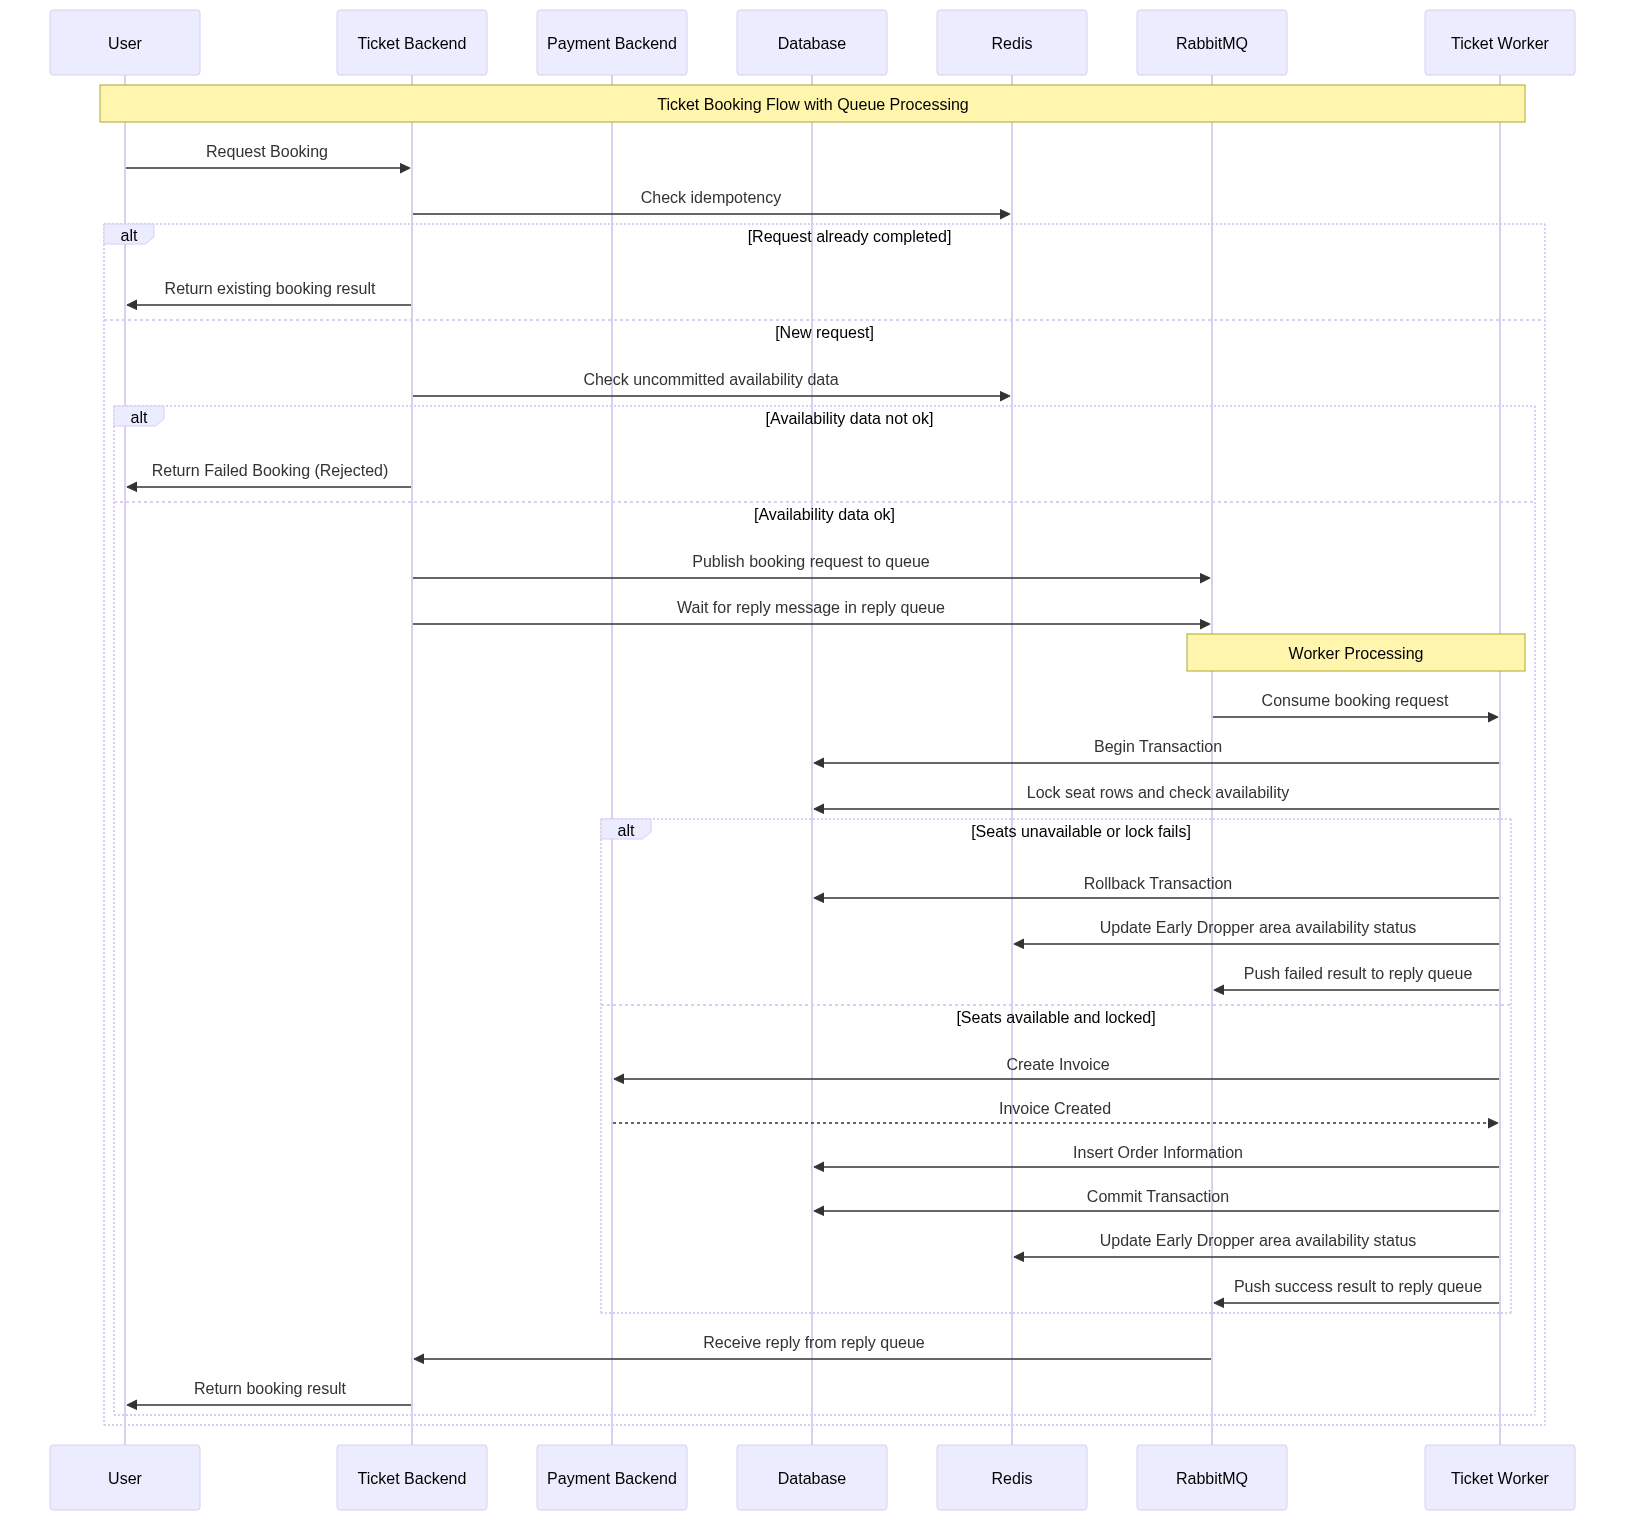
\includegraphics[width=1\textwidth]{resources/chapter-3/book-async.png}
    \caption{Diagram Alur Fitur Pemesanan Tiket (dengan pengendalian aliran)}
    \label{fig:flow-book-fc}
\end{figure}

\pagebreak

Ketika pengguna berhasil memesan, pengguna akan melakukan pembayaran kepada gerbang pembayaran. Setelah pembayaran selesai, pengguna memeriksa status pesanan yang telah dibuat. Tidak ada perbedaan signifikan selain pembaruan data pada Redis untuk sinkronisasi data yang menjadi basis untuk menolak permintaan pesanan lebih awal.

\begin{figure}[h]
    \centering
    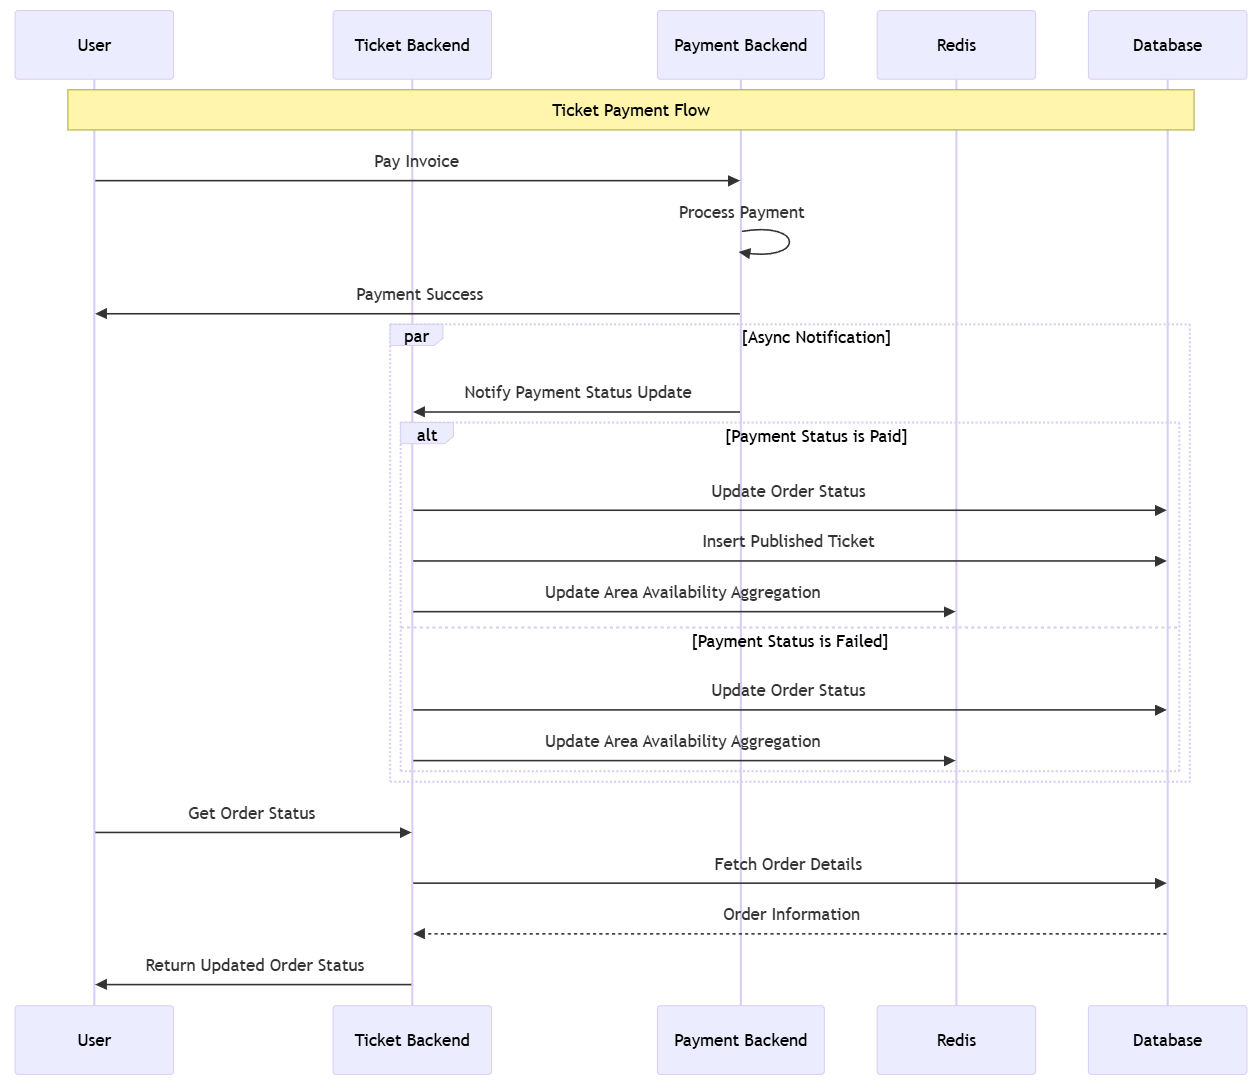
\includegraphics[width=1\textwidth]{resources/chapter-3/order-payment.png}
    \caption{Diagram Alur Fitur Pembayaran Tiket (tanpa pengendalian aliran)}
    \label{fig:flow-order-payment-fc}
\end{figure}

\pagebreak

\subsubsection{Alur Fitur Pembacaan Pesanan}

Terdapat dua operasi tambahan yang berkaitan dengan pembacaan pesanan, yaitu membaca detail pesanan dan membaca tiket yang sudah diterbitkan.

\begin{figure}[h]
    \centering
    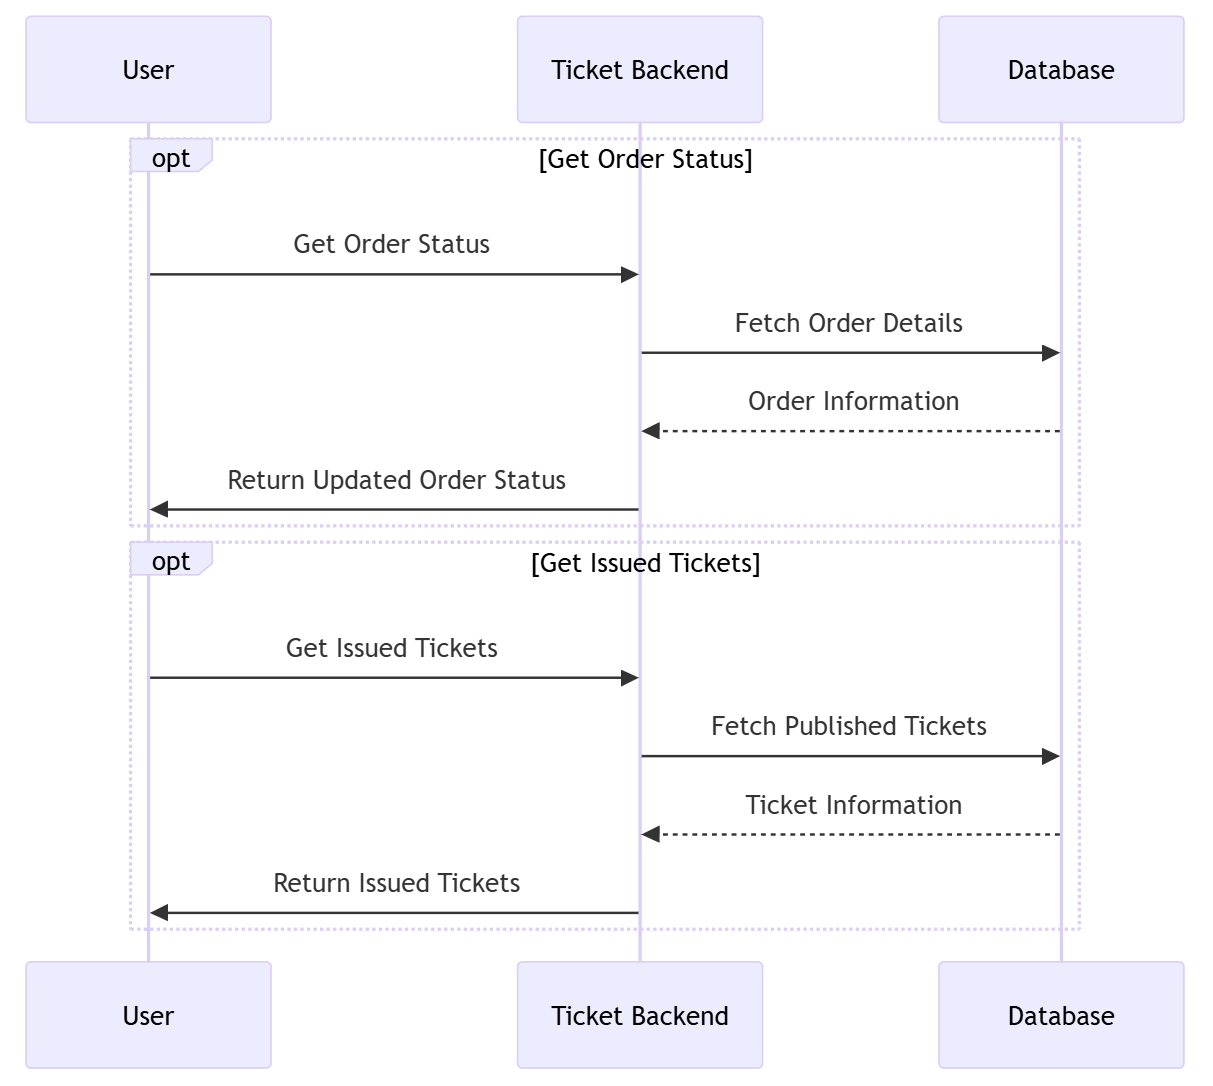
\includegraphics[width=1\textwidth]{resources/chapter-3/order-flow.png}
    \caption{Diagram Alur Fitur Pembacaan Pesanan}
    \label{fig:flow-order-flow}
\end{figure}

\chapter{Arsitektur Solusi}

Komponen \textit{backend} utama bersifat \textit{stateless}, sehingga dapat di-\textit{scale} dengan meningkatkan jumlah \textit{instance}. Setiap arsitektur solusi memiliki dua layanan eksternal, yaitu layanan pengguna dan layanan gerbang pembayaran. Basis data merupakan komponen yang sulit di-\textit{scale} secara dinamis berdasarkan beban yang diterima. Biasanya, penskalaan secara vertikal merupakan opsi utama untuk meningkatkan \textit{throughput}.

\section{Arsitektur Dasar Acuan}

\begin{figure}[ht]
    \centering
    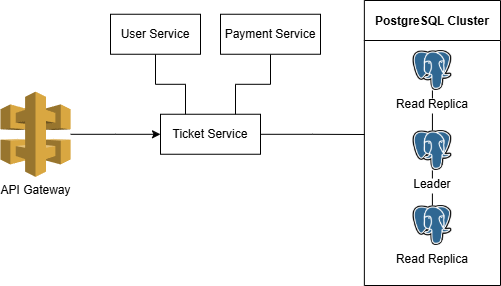
\includegraphics[width=0.8\textwidth]{resources/chapter-3/architecture-reference.png}
    \caption{Arsitektur Dasar Acuan}
    \label{fig:baseline-architecture}
\end{figure}

Arsitektur ini akan menjadi dasar acuan yang digunakan sebagai dasar perbandingan kinerja. Terdapat kluster PostgreSQL dengan konfigurasi satu node pemimpin dan sisanya node replika. Keberadaan replika memungkinkan peningkatan \textit{throughput} permintaan baca, tetapi tidak ada pengoptimalan untuk operasi tulis.

\section{Arsitektur yang Mengoptimalkan PostgreSQL}

Arsitektur ini mengoptimalkan sistem dengan pola CQRS. Tanggung jawab permintaan baca dilimpahkan kepada RisingWave. \textit{Streaming database} ini mengonsumsi \textit{CDC stream} dari kluster PostgreSQL, lalu memperbarui kueri secara inkremental. Penggunaan ekstensi Citus memungkinkan pembagian data berdasarkan baris dan \textit{multiple writer}. Selain itu, perintah pemesanan tiket (berupa \textit{command}/ \textit{event sourcing}) akan dimasukkan ke dalam antrean terlebih dahulu, lalu diproses secara bertahap. Redis digunakan untuk menyimpan \textit{uncommited data} dan menolak permintaan pemesanan lebih awal.

\begin{figure}[ht]
    \centering
    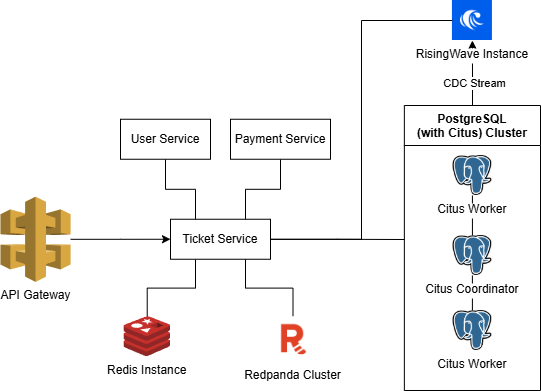
\includegraphics[width=0.8\textwidth]{resources/chapter-3/architecture-optimized.png}
    \caption{Arsitektur yang Mengoptimalkan PostgreSQL}
    \label{fig:optimized-architecture}
\end{figure}

Penggunaan ekstensi Citus memungkinkan penginkatan \textit{write throughput} tidak hanya dengan pendekatan \textit{scale up}, tetapi juga dengan pendekatan \textit{scale-out}. Redpanda dapat dibuat kluster dengan pemartisian data untuk meningkatkan \textit{throughput}. Redis dapat dikonfigurasikan dalam mode kluster untuk redundansi dan mode AOF untuk \textit{persistence}.

\section{Arsitektur \textit{Event-Driven}}

Arsitektur ini tidak menggunakan PostgreSQL sama sekali. Pada dasarnya, basis data relasional terdiri atas komponen \textit{storage} dan \textit{query processor}. Pada arsitektur ini, komponen \textit{storage} diganti menggunakan Redpanda dengan berbagai topik dan \textit{query processor} diganti dengan RisingWave. Meskipun begitu, pendekatan ini tidak memiliki dukungan \textit{transaction} selain \textit{transaction} pada Redpanda yang berupa \textit{push log all or nothing} pada beberapa topik sekaligus. Untuk itu, Redis digunakan untuk menyimpan \textit{dirty data} atau \textit{uncommited data} sehingga untuk mencegah \textit{double booking}.

\begin{figure}[ht]
    \centering
    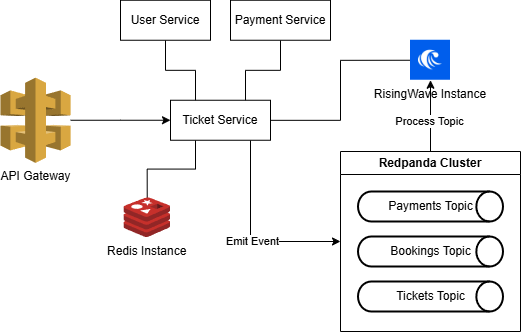
\includegraphics[width=0.8\textwidth]{resources/chapter-3/architecture-event-driven.png}
    \caption{Arsitektur \textit{Event-Driven}}
    \label{fig:solution-event-driven-architecture}
\end{figure}

Redpanda dapat dibuat kluster dengan pemartisian data untuk meningkatkan \textit{throughput}. Redis dapat dikonfigurasikan dalam mode kluster untuk redundansi dan mode AOF untuk \textit{persistence}. Selain itu, RisingWave merupakan \textit{streaming database} yang \textit{cloud-native} sehingga dapat di-\textit{scale out} dengan mudah untuk meningkatkan \textit{throughput}.



\pagebreak

\section{Rencana Pengujian}

\subsection{Metodologi Pengujian Sistem}

Untuk mengevaluasi dan mengoptimalkan sistem tiket, metodologi pengujian dirancang untuk menyimulasikan kondisi operasional di dunia nyata secara akurat. Fokus utama pengujian adalah memastikan sistem mampu menangani skenario beban tinggi dengan andal. Metodologi ini mencakup aspek-aspek berikut:

\begin{enumerate}
    \item \textbf{Simulasi beban realistis pada skala besar:} Pengujian dilakukan dengan beban yang melampaui kapasitas satu server tunggal.
    \item \textbf{Simulasi perilaku pengguna:} Pengujian dilakukan dengan penggunaan pengguna virtual yang memiliki alur aksi serta profil pengguna yang beragam. Setiap pengguna virtual diberi profil tertentu untuk meniru keberagaman perilaku pembeli di dunia nyata.
    \item \textbf{Skenario penjualan:} Data acara dan distribusi kuota tiket diambil dari estimasi yang merepresentasikan penjualan tiket populer di dunia nyata. Distribusi kursi setiap kategori tidak akan sama dengan distribusi minat pembeli. Hal ini wajar karena pada kenyataannya memang terdapat kategori tertentu yang lebih ramai peminat dibandingkan dengan kategori yang lain.
    \item \textbf{Skenario Pengujian:} Dua skenario pengujian disiapkan untuk menganalisis kinerja sistem, yaitu pengujian beban berkelanjutan dan pengujian perebutan tiket.
\end{enumerate}


\pagebreak

\subsection{Simulasi Pengguna}

Berikut adalah alur simulasi pengguna. Alur dimulai dengan pengguna mengambil data acara, dilanjutkan dengan membaca data ketersediaan berdasarkan area dan kursi. Proses dilanjutkan dengan pemesanan, pembayaran, hingga pemesanan berhasil atau gagal (yang disimulasikan).

\begin{figure}[htbp]
    \centering
    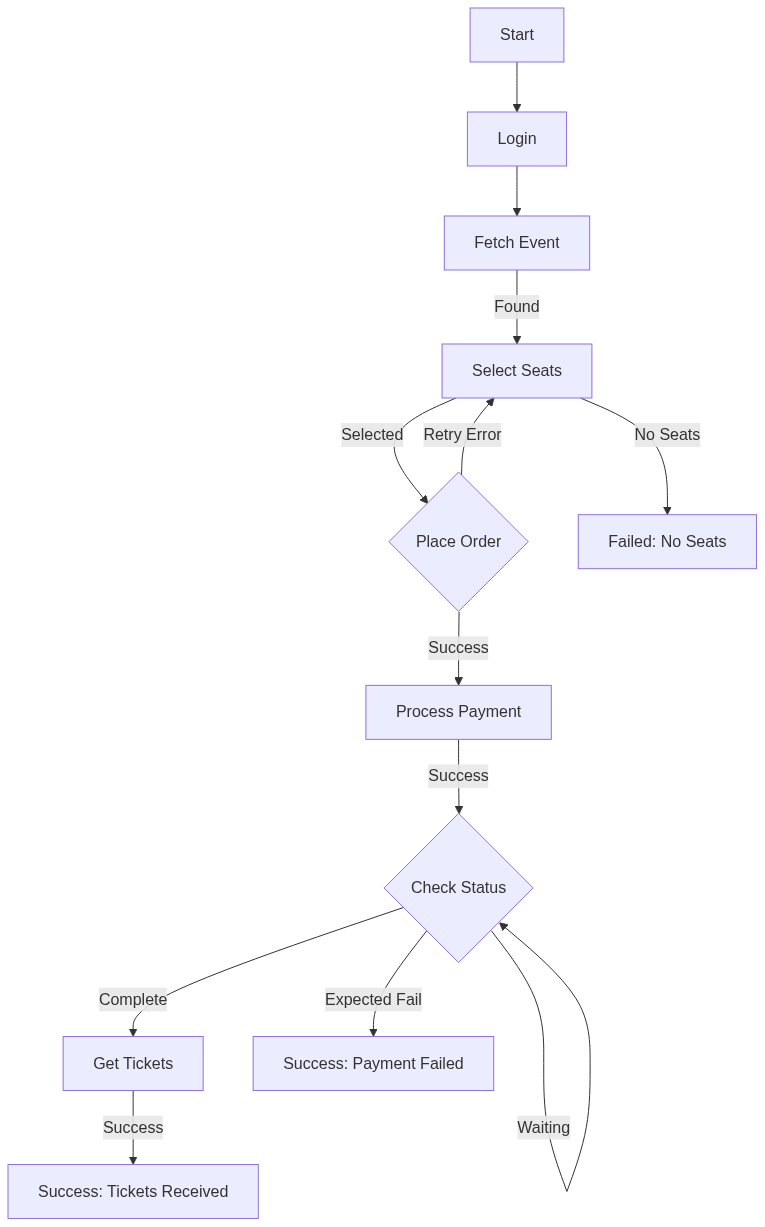
\includegraphics[width=0.7\textwidth]{resources/chapter-3/user-flow.png}
    \caption{Alur Simulasi Pengguna}
    \label{fig:user-flow}
\end{figure}

\pagebreak

\subsection{Distribusi Profil Pengguna}

Ketika pengguna berhasil memesan tiket, terdapat 5\% kemungkinan bahwa pembayaran pengguna gagal. Hal ini dilakukan untuk menyimulasikan pengguna yang batal membeli tiket atau mengalami kegagalan pembayaran. Meskipun begitu, tidak ada referensi pasti yang menyebutkan tingkat kegagalan pemesanan untuk penjualan tiket. Sebagai referensi, tingkat kegagalan pemrosesan transaksi pada \textit{e-commerce} berkisar pada 11\% \parencite{paymentFail}. Meskipun begitu, angka yang lebih rendah diambil karena pada kasus ini pengguna yang mendaftar memiliki keinginan yang lebih kuat untuk memperoleh tiket.

Distribusi preferensi kategori tiket, sebagaimana dirinci pada Tabel \ref{table:distribusi-kategori}, didasarkan pada teori diskriminasi harga (\textit{tiered pricing}) \parencite{acei2022}. Pendekatan ini biasanya digunakan oleh penyelenggara untuk memaksimalkan pendapatan dengan mensegmentasi pasar berdasarkan kesediaan untuk membayar (\textit{willingness to pay}). Sebagian besar permintaan (53\%) terkonsentrasi pada tingkatan harga menengah ke bawah (\textit{Seated Low \& Mid}), yang mencerminkan segmen pasar yang lebih besar dan sensitif terhadap harga. Sebaliknya, profil dengan minat pada kategori harga lebih tinggi merepresentasikan segmen pasar yang lebih kecil dan kurang sensitif terhadap harga untuk tiket yang lebih mahal.

\begin{table}[H]
    \centering
    \caption{Distribusi Kategori}
    \label{table:distribusi-kategori}
    \begin{tabular}{|l|l|l|}
        \hline
        \textbf{Tingkatan} & \textbf{Distribusi} & \textbf{Minat Kategori} \\
        \hline
        Seated Low         & 27\%                & Bronze \& Silver        \\
        \hline
        Seated Mid         & 26\%                & Silver, Gold, \& Bronze \\
        \hline
        Seated High        & 19\%                & Platinum \& Gold        \\
        \hline
        Area Mid           & 17\%                & Zona A \& Zona B        \\
        \hline
        Area High          & 11\%                & VIP \& Zona A           \\
        \hline
    \end{tabular}
\end{table}

Preferensi hari acara dibagi menjadi 52\% "Spesifik" dan 48\% "Bebas" (\textit{Any}), seperti pada Tabel \ref{table:distribusi-hari}. Pembagian ini mencerminkan keseimbangan antara penonton dengan jadwal yang kaku dan mereka yang memiliki fleksibilitas. Terdapat preferensi konsumen yang kuat untuk acara rekreasi pada akhir pekan karena berbagai komitmen sosial dan pekerjaan \parencite{rgate2013}. Kelompok "Spesifik" mewakili mereka yang terikat pada hari tertentu, sementara kelompok "Bebas" mewakili penggemar yang lebih fleksibel atau sangat termotivasi untuk mendapatkan tiket.

\begin{table}[H]
    \centering
    \caption{Distribusi Hari}
    \label{table:distribusi-hari}
    \begin{tabular}{|l|l|}
        \hline
        \textbf{Hari} & \textbf{Distribusi} \\
        \hline
        Specific      & 52\%                \\
        \hline
        Any           & 48\%                \\
        \hline
    \end{tabular}
\end{table}

Variasi berikutnya adalah variasi dari seberapa persisten pengguna untuk mendapatkan tiket yang diinginkan. Variasi ini ditentukan dengan berapa kali maksimal pencarian dan pemesanan sebelum pengguna tersebut menyerah. Distribusi persistensi pengguna dibahas pada Tabel \ref{table:distribusi-persistensi}.

\begin{table}[H]
    \centering
    \caption{Distribusi Persistensi}
    \label{table:distribusi-persistensi}
    \begin{tabular}{|l|l|l|}
        \hline
        \textbf{Persistence} & \textbf{Distribusi} & \textbf{Batas}                      \\
        \hline
        Low                  & 19\%                & 9x pencarian atau 3x pemesanan      \\
        \hline
        Medium               & 51\%                & 18x pencarian atau 6x     pemesanan \\
        \hline
        High                 & 30\%                & 27x pencarian atau 9x pemesanan     \\
        \hline
    \end{tabular}
\end{table}

Variasi terakhir adalah variasi dari berapa banyak tiket yang dipesan oleh suatu pengguna dalam satu kali pemesanan. Hal ini untuk menyimulasikan pengguna yang datang sendiri, bersama pasangan, dan datang dalam satu grup. Distribusi ini dibahas pada Tabel \ref{table:distribusi-kuantitas}. Model ini menghasilkan rata-rata tertimbang 2-3 tiket per transaksi, yang sangat selaras dengan data dari industri hiburan lain, seperti penjualan tiket film yang menunjukkan rata-rata 2.3 tiket per transaksi \parencite{vista2025}.

\begin{table}[H]
    \centering
    \caption{Distribusi Kuantitas}
    \label{table:distribusi-kuantitas}
    \begin{tabular}{|l|l|l|}
        \hline
        \textbf{Varian} & \textbf{Distribusi} & \textbf{Kuantitas} \\
        \hline
        Solo            & 28\%                & 1                  \\
        \hline
        Couple          & 48\%                & 2                  \\
        \hline
        Group           & 24\%                & 3-5                \\
        \hline
    \end{tabular}
\end{table}

Distribusi kombinasi setiap variasi di atas disertakan pada Lampiran \ref{apx:distribusi-profil}.

\subsection{Variasi Data Penjualan Tiket}

Terdapat dua skenario yang akan digunakan selama pengujian, yaitu:

\begin{enumerate}
    \item Skenario sf-4, yaitu skenario skala penuh (80.000 tiket per hari) yang diselenggarakan selama 4 hari. Total kursi yang dijual adalah 320.000.
    \item Skenario s10-2. Skenario skala satu berbanding sepuluh (8.000 tiket per hari) yang diselenggarakan selama 2 hari. Total data kursi yang dijual adalah sekitar 16.000.
\end{enumerate}

\subsection{Skenario Pengujian}

Terdapat dua jenis skenario pengujian yang akan diuji pada penelitian ini, yaitu skenario beban berkelanjutan (\textit{load test}) dan skenario perebutan tiket. Keduanya memiliki pendekatan dan tujuan yang berbeda.

\subsubsection{Skenario Beban Berkelanjutan}

Skenario ini berfokus pada jumlah pengguna virtual dalam satu waktu (\textit{concurrent virtual user}). Pada skenario ini, sistem akan dibebankan sejumlah pengguna virtual dengan durasi tertentu. Meskipun begitu, skenario ini tidak menunjukkan keadaan perebutan tiket sebagiamana terjadi pada kehidupan nyata.

\subsubsection{Skenario Perebutan Tiket}

Skenario ini menguji beberapa hal, seperti pengujian lonjakan dan perilaku sistem pada saat terjadi perebutan tiket. Tes ini terinspirasi dari rasio antara pengguna dengan tiket yang dijual. Rasio ini sangat tinggi karena ada banyak pengguna yang menginginkan satu tiket.

Skenario ini berfokus pada jumlah kedatangan (\textit{arrival rate}) alih-alih jumlah pengguna virtual dalam satu waktu. Skenario ini dibuat dengan cara berikut:

\begin{enumerate}
    \item Estimasikan jumlah pengguna dan jumlah tiket yang dijual. Misalkan terdapat 40 ribu iterasi pengguna dan 16 ribu tiket yang dijual.
    \item Distribusikan kedatangan pengguna berdasarkan distribusi tertentu. Penelitian ini menggunakan distribusi lognormal untuk menyimulasikan lonjakan. Total area di bawah kurva akan sama dengan jumlah pengguna. Lebar kurva merupakan durasi pengujian dengan tinggi kurva merupakan jumlah kedatangan pengguna pada waktu tertentu. Untuk mempermudah implementasi, kedatangan pengguna dibagi secara periodik, misalkan setiap 30 detik.
    \item Hasil grafik distribusi digunakan untuk menentukan banyaknya kedatangan pengguna pada waktu tertentu.
\end{enumerate}


% \chapter{Implementasi dan Pengujian}
Bab ini akan menjelaskan proses implementasi dari rancangan solusi yang telah dikaji pada Bab III. Setelah pembahasan terkait implementasi, akan dilanjutkan dengan pemaparan hasil uji terkait implementasi yang telah dibuat.

\section{Implementasi}

\subsection{Batasan Implementasi}

Berikut adalah batasan yang ditetapkan dalam melakukan implementasi sistem ini.

\begin{enumerate}
  \item Semua batasan masalah dan konfigurasi yang telah dibahas pada Subbab \ref{sec:batasan-masalah}.
  \item Layanan pengguna tidak diimplementasikan sebagaimana dibahas pada bagian rancangan solusi.
  \item Setiap layanan yang diimplementasikan hanya berupa REST API Endpoint yang akan dipanggil secara langsung oleh pengguna virtual. Antarmuka sistem tidak diimplementasikan karena dinilai tidak relevan dengan fokus pengujian.
  \item Sistem dikembangkan dengan orientasi \textit{deployment} menggunakan kluster Kubernetes.
\end{enumerate}


\subsection{Lingkungan Pengembangan}

\subsubsection{Lingkungan Pengembangan}

Tugas akhir ini dikembangkan pada perangkat laptop Asus TUF A15 FA506IC dengan spesifikasi sebagai berikut:

\begin{enumerate}
    \item Processor: AMD Ryzen 7 4800H 8 core 16 thread.
    \item RAM: 24GB DDR4 3200MHz.
    \item Windows 11 dengan WSL2 Ubuntu 22.04.
    \item Penyimpanan: 500GB + 1TB SSD NVME.
\end{enumerate}

\subsubsection{Lingkungan Pengujian Lokal}

Lingkungan pengujian lokal memiliki dua pengujian:

\begin{enumerate}
    \item \textit{Integration test} dilakukan pada Ubuntu 22.04 WSL2 dengan Docker Engine untuk orkestrasi dependensi.
    \item \textit{End-to-end testing} dilakukan pada dua kluster kubernetes lokal dengan bantuan K3d (sebuah abstraksi untuk menjalankan K3s sebagai Docker container). Versi image k3s yang digunakan adalah v1.30.12-rc1-k3s1.
          \begin{enumerate}
              \item Sistem backend dengan 1 node control plane dan 1 node worker.
              \item Agen penguji dengan 1 node control plane dan tanpa node worker.
          \end{enumerate}
\end{enumerate}


\subsection{Kakas yang Digunakan}

\subsubsection{Layanan Pembayaran}

Node.JS 20
TypeScript
Hono sebagai HTTP Framework
BullMQ sebagai kakas Message Queue di atas Redis

\subsection{Layanan Tiket}

Golang 1.24.0
Golang Echo sebagai HTTP Framework
TestContainers untuk integration testing
Go Concurrency Limits
PGX Postgres Driver Library
BigCache untuk in-memory cache
UberFX untuk dependency injection

\subsection{Kakas Deployment dan Pengawasan}

Dideploy pada kluster Kubernetes.
Grafana Loki untuk log collection.
Grafana Alloy untuk log collector.
Grafana Dashboard untuk visualisasi.
Prometheus untuk metrics collection.

Exporter spesifik untuk metrics collection, seperti PostgreSQL prometheus exporter.

\subsection{Lainnya}

Grafana K6 untuk library load testing
Grafana K6 Operator untuk deployment di Kubernetes.
TypeSpec untuk membuat dokumentasi OpenAPI
Integrasi Prometheus untuk metrics collection



% \subsection{Kakas yang Digunakan}
Dalam melakukan implementasi ini diperlukan beberapa kakas, diantaranya adalah sebagai berikut.
\begin{enumerate}
  \item \textit{Docker}, \textit{Docker Desktop} dan \textit{Kind} untuk dipakai sebagai \textit{containerization} dan \textit{cluster} kubernetes lokal.
  \item Implementasi \textit{service} bahasa pemrograman golang dan menggunakan beberapa kakas berikut
        \begin{enumerate}
          \item \textit{Kubernetes Go Client} untuk mengontrol \textit{cluster} kubernetes melalui kode Golang.
          \item \textit{Echo} sebagai \textit{server framework}
          \item \textit{Logrus} sebagai logger dari setiap aksi pada sistem
          \item \textit{Cobra dan Viper} sebagai \textit{CLI command} pada golang untuk memudahkan pemilihan \textit{entrypoint} dan \textit{environment variables}
          \item \textit{PQ, Sqlx, Go-migrate} sebagai kakas yang menghubungkan sistem dengan \textit{database}. Sqlx merupakan ekstensi dari library \textit{database/sql} milik golang. Go migrate digunakan untuk melakukan migrasi dari schema sql yang telah dibuat dan melakukan keep track dari versi schema yang sedang digunakan
          \item \textit{Validator} digunakan untuk memvalidasi \textit{request} yang masuk
        \end{enumerate}

  \item Implementasi \textit{dashboard} menggunakan \textit{vue} dan \textit{typescript} dan \textit{nuxt} sebagai framework.
        \begin{enumerate}
          \item \textit{NuxtUI} Sebagai kakas untuk memudahkan pembuatan \textit{UI}.
          \item \textit{Pinia} Sebagai kakas untuk manajemen data \textit{UI}.
          \item \textit{Zod} Sebagai object schema validator sebelum mengirimkan request.
        \end{enumerate}
\end{enumerate}

% \subsection{Persiapan \textit{kubernetes cluster}}
\label{subsec:persiapan-kubernetes-cluster}

Tahapan ini merupakan tahapan persiaspan sebelum proses \textit{development}. Pada tahapan ini dibuat kubernetes \textit{cluster} pada komputer lokal dengan kakas \textit{kind}. \textit{Cluster} yang dibuat memiliki 4 nodes dengan spesifikasi 1 \textit{master node} dan 3 \textit{worker node}. Digunakan \textit{command} kind create cluster --config cluster.yaml dengan file konfigurasi yang dapat dilihat pada gambar \ref{fig:konfigurasi-pembuatan-cluster}. Setelah berhasil di \textit{apply}, muncul 4 buah kontainer yang dapat berfungsi sebagai \textit{kubernetes cluster} seperti pada gamabar \ref{fig:hasil-cluster-kind}.

\begin{figure}[ht]
  \centering
  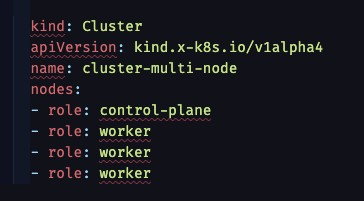
\includegraphics[width=1\textwidth]{resources/appendix/pembuatan-cluster.jpg}
  \caption{Konfigurasi Pembuatan \textit{Kubernetes Cluster} dengan \textit{Kind}}
  \label{fig:konfigurasi-pembuatan-cluster}
\end{figure}

\begin{figure}[ht]
  \centering
  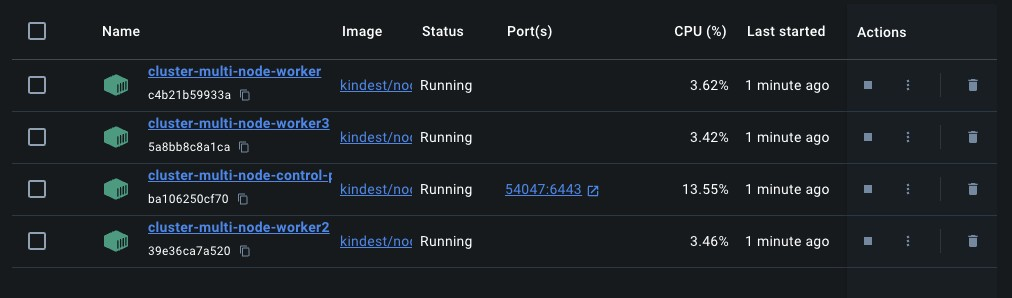
\includegraphics[width=1\textwidth]{resources/chapter-4/cluster-kind.jpg}
  \caption{Hasil \textit{Kubernetes Cluster} Dengan Kakas \textit{Kind}}
  \label{fig:hasil-cluster-kind}
\end{figure}

\pagebreak

% \subsection{Implementasi \textit{Dashboard}}
Komponen \textit{dashboard} dibuat dengan menggunakan bahasa pemrogramman \textit{typescript} dan \textit{vue}. Framework yang digunakan dalam membuat \textit{Dashboard} adalah \textit{Nuxt}. \textit{Nuxt} menjadi pilihan karena memiliki \textit{developer experience} yang bagus serta fitur yang cukup lengkap. \textit{Nuxt} juga memiliki \textit{UI library} yaitu \textit{NuxtUI} yang memudahkan pembuatan \textit{UI}. Pada komponen ini, terdapat 10 halaman yang dapat dikunjungi oleh \textit{user}. Detail dari penjelasan setiap halaman dapat ditemukan pada subbab dibawah ini.

\subsubsection{Halaman \textit{Login}}
Halaman ini berada pada \textit{route} /login. Halaman ini yang berfungsi sebagai \textit{entrypoint} dari komponen \textit{dashboard}. Pada halaman ini terdapat dua input yang di \textit{wrap} oleh sebuah \textit{form}. Input berupa \textit{email} dan \textit{password} \textit{user}. Setelah \textit{user} memasukan \textit{email} dan \textit{password} yang sesuai, maka dilakukan \textit{redirect} ke laman utama untuk menunjukan bahwa \textit{user} berhasil terautentikasi dan menggunakan fungsionalitas \textit{dashboard}. Tampilan halaman ini dapat dilihat pada lampiran \ref{fig:halaman-login}.

\subsubsection{Halaman utama}
Halaman ini merupakan halaman utama dari komponen \textit{dashboard}. Pada halaman ini \textit{user} dapat melihat status dari masing masing objek mulai dari \textit{deployment}, \textit{device}, \textit{group}, serta \textit{quick actions} untuk menuju halaman terkait.

\subsubsection{Halaman \textit{Account}}
Halaman ini berada pada \textit{route /account}. Halaman ini berfungsi untuk memberikan detail mengenai \textit{company} dari \textit{user}. Informasi \textit{company} ditampilkan pada sebuah \textit{card} yang berada pada tengah halaman. Pada halaman ini juga ditampilkan informasi mengenai daftar \textit{user} yang berada pada \textit{company} yang sama dan ditampilkan dengan sebuah tabel. Tampilan halaman ini dapat dilihat pada lampiran \ref{fig:halaman-account}.

\subsubsection{Halaman \textit{Device}}
Halaman ini berada pada \textit{route /devices}. Halaman ini berfungsi untuk melakukan manajemen \textit{device} pada satu perusahaan. Halaman ini menunjukan informasi seluruh \textit{device} yang terdaftar pada \textit{company}. Tampilan halaman ini dapat dilihat pada lampiran \ref{fig:halaman-device}.

Sama seperti halaman \textit{account}, terdapat tombol dengan icon elipsis pada bagian kanan untuk melakukan fungsi seperti melihat detail ataupun menghapus \textit{device} terkait. Apabila \textit{user} menekan tombol \textit{detail} maka user diarahkan ke halaman /device/:id sesuai dengan id \textit{device} yang dipilih. Tombol yang dimaksud dapat dilihat pada lampiran \ref{fig:halaman-device-actions}.

Pada halaman ini terdapat tombol yang dapat ditekan untuk menambahkan \textit{device}. Apabila ditekan muncul sebuah modal yang berisi input yang dapat \textit{user} isi untuk membuat sebuah \textit{device} baru pada sistem. Terdapat validasi pada setiap input, setelah semua validasi dilewati, tombol \textit{submit} mengirimkan \textit{request} ke \textit{server} untuk di proses. Tombol yang dimaksud dapat dilihat pada lampiran \ref{fig:halaman-device-add}.

Akan muncul sebuah notifikasi pada bagian kanan bawah tergantung \textit{response} yang diberikan oleh \textit{server}. Warna hijau menandakan bahwa \textit{response} sukses dan warna \textit{merah} menandakan bahwa terdapat masalah ketika memproses \textit{request}.

\subsubsection{Halaman \textit{Device detail}}
Halaman ini dapat diakses dengan cara mengunjungi /devices/:id dari tombol \textit{detail} pada \textit{actions} yang berada pada halaman /devices. Pada halaman ini \textit{user} dapat menambahkan \textit{device} ke dalam sebuah group dengan menekan tombol \textit{add group}. Halaman dapat dilhat pada lampiran \ref{fig:halaman-device-detail}.

Modal \textit{add group} muncul jika tombol ditekan, modal ini memliki sebuah dropdown yang telah berisi \textit{group} yang tersedia pada sistem. Akan muncul sebuah notifikasi pada bagian bawah kanan untuk menandakan bahwa \textit{request} berhasil di proses oleh server. Warna hijau menandakan sukses dan warna merah menandakan bawhwa \textit{server} belum berhasil memproses permintaan tersebut. Modal dapat dilhat pada lampiran \ref{fig:halaman-device-detail-add-group}.

Pada halaman ini juga terdapat tombol \textit{delete} yang berada pada pojok kanan atas. Jika \textit{user} memutuskan untuk menghapus \textit{device}, muncul sebuah modal konfirmasi sebelum aksi penghapusan dilakukan. Modal dapat dilihat pada lampiran \ref{fig:halaman-device-detail-delete}.

\subsubsection{Halaman \textit{Groups}}
Halaman ini berada pada \textit{route /groups}. Halaman ini menunjukan informasi mengenai \textit{groups} yang telah terdaftar pada sistem. Informasi ditampilkan dalam bentuk tabel yang berisi detail dari objek \textit{groups}. Halaman dapat dilihat pada lampiran \ref{fig:halaman-groups}.

Pada tabel terdapat tombol elipsis yang terletak pada bagian kanan dari masing masing \textit{row}. Sama seperti tabel lainnya, tombol ini berfungsi untuk melakukan \textit{action} pada \textit{row}. Aksi yang dapat dilakukan berupa mengakses halaman detail atau menghapus \textit{item} tersebut.

Apabila tombol \textit{detail} dipilh maka \textit{user} menuju halaman \textit{group detail}. Apabila tombol \textit{delete} dipilih maka \textit{item} dihapus dari sistem dan muncul notifikasi pada bagian bawah yang menandkana bahwa proses berhasil dilakukan. Tombol dapat dilhat pada lampiran \ref{fig:halaman-groups-actions}.

Pada halaman ini juga \textit{user} dapat menambahkan \textit{groups} dengan menekan tombol \textit{add group}. Ketika tombol ini ditekan, muncul modal yang memiliki input nama. Input ini memiliki validasi berupa panjang karakter yang dimasukan haruslah memiliki panjang minimal 8 karakter. Tombol submit berfungsi untuk mengirimkan \textit{request} ke server. Akan muncul notifikasi pada bagian bawah kanan untuk menandakan bahwa \textit{request} berhasil di proses. Warna hijau menandakan bahwa \textit{request} berhasil di proses dan warna merah menandakan sebaliknya. Modal dapat dilihat pada lampiran \ref{fig:halaman-groups-add}.

\subsubsection{Halaman \textit{Groups detail}}
Halaman ini dapat diakses oleh \textit{pengguna} melalui tombol \textit{detail} yang ada pada tabel di halaman \textit{groups}. Halaman ini memiliki \textit{route /groups/:id}. Pada halaman ini \textit{user} dapat melihat informasi mengenai detail dari \textit{groups} yang dipilih mulai dari nama, deskripsi dan \textit{device} apa saja yang telah terhubung pada \textit{group tersebut}. Halaman dapat dilihat pada lampiran \ref{fig:halaman-groups-detail}.

\textit{user} juga dapat menambahkan \textit{device} dengan cara menekan tombol \textit{add devices} yang memunculkan modal berisi dropdown seluruh perangkat yang belum memiliki \textit{groups}. \textit{Dropdown} dapat dilihat pada lampiran \ref{fig:halaman-groups-detail-add-group} dan \ref{fig:halaman-groups-detail-delete}.

\subsubsection{Halaman \textit{Deployment}}
Halaman ini merupakan fungsionalitas utama dari sistem \textit{remote deployment}. Halaman ini dapat diakses melalui \textit{sidebar} dan memiliki \textit{route /deployments}. Pada halaman ini \textit{user} dapat melihat informasi mengenai \textit{deployment plan} yang terdaftar pada sistem. Selain itu juga terdapat informasi mengenai \textit{deployment images} yang tersedia dalam sistem. Kedua informasi ditampilkan dalam bentuk tabel yang masing masing memiliki tombol \textit{add} pada bagian kanan bawah tabel. Halaman dapat dilihat pada lampiran \ref{fig:halaman-deployment}.

Tombol add tersebut memunculkan modal yang berisi input yang harus diisi jika ingin membuat \textit{item} baru. Sama seperti tabel lainnya, pada masing masing tabel terdapat tombol elipsis pada bagian kanan untuk melakukan aksi berupa melihat \textit{detail} ataupun menghapus \textit{item} yang bersesuaian. Tampilan tombol dapat dilihat pada lampiran \ref{fig:halaman-deployment-add-deployment} dan \ref{fig:halaman-deployment-add-repostory}.

\subsubsection{Halaman \textit{deployments detail}}
Halaman ini dapat diakses melalui tombol \textit{detail} di tabel \textit{deployment} pada halaman \textit{deployment}. Halaman ini memiliki \textit{route /deployments/:id}. Halaman ini menunjukan informasi mengenai \textit{deployment} yang telah dilakukan, status dari \textit{deployment}, serta target dari \textit{deployment} tersebut. Tampilan halaman dapat dilihat pada lampiran \ref{fig:halaman-deployment-detail}.

Pada halaman ini juga terdapat tombol \textit{delete} yang berada pada pojok kanan atas. Dengan menekan tombol ini muncul sebuah modal untuk melakukan konfirmasi jika ingin menghapus \textit{deployment}. Tampilan dapat dilihat pada lampiran \ref{fig:halaman-deployment-detail-delete}.

\subsubsection{Halaman \textit{FAQ}}
Halaman ini berada pada \textit{route /faq}. Halaman ini bertujuan untuk memberikan informasi mengenai tata cara hal yang perlu dilakukan sebelum mendaftarkan \textit{device} ke sistem. Terdapat dua bagian yang dibedakan dari banyaknya \textit{device} yang terhubung ke dalam sistem. Dua kategori tersebut yaitu jika belum memiliki \textit{device} sama sekali dan memiliki setidaknya 1 \textit{device} yang telah terhubung dengan sistem.


% \subsection{Implementasi \textit{Service}}
\label{subsec:implementasi-service}

Implementasi \textit{service} dibuat dengan menggunakan bahasa pemrogramman golang dan framework \textit{Echo} serta menggunakan \textit{REST API} sebagai gaya komunikasinya. Arsitektur kode yang dibuat memiliki tiga lapisan dimulai dari \textit{handler}, \textit{usecase}, dan \textit{repository}. Handler bertujuan membaca permintaan pengguna dan dapat disebut sebagai entrypoint. Data dari handler diberikan kepada \textit{usecase} untuk diproses. \textit{Usecase} merupakan lapisan yang hanya memiliki \textit{logic} proses bisnis. Setelah data berhasil melewati lapisan \textit{usecase}, data siap untuk dimasukkan ke database. Proses hubungan antara \textit{service} dengan \textit{database} diletakan pada lapisan \textit{repository}.

Pemisahan lapisan ini mengikuti design pattern yaitu \textit{dependency injection}. Selain itu, pemisahan ini juga bertujuan memudahkan testing dan meningkatkan \textit{maintanability} karena mudah untuk dibaca dan dipahami. \textit{endpoint} dibuat dengan menggunakan versioning dengan base \textit{endpoint} /v1. Versioning digunakan untuk memudahkan penggantian endpoint jika suatu saat terdapat perubahan major yang bersifat \textit{breaking}. Selain itu base \textit{endpoint} untuk \textit{user} dan \textit{admin} memiliki perbedaan pada prefix /api dan /admin-api

Pada sistem ini terdapat \textit{middleware} yang digunakan untuk melakukan otorisasi \textit{pengguna}. Berikut merupakan daftar dan penjelasan \textit{middleware} pada sistem

\begin{enumerate}
    \item ValidateAPIKey

          \textit{Middleware} ini bertujuan untuk memastikan bahwa hanya \textit{client} yang sesuai lah yang dapat mengakses \textit{service}. API Key dikirimkan dengan cara meletakan pada header dengan key X-API-Key. Middleware ini dijalankan untuk seluruh \textit{endpoint} yang ada pada \textit{service}.

    \item ValidateJWTKey

          \textit{Middleware} ini memiliki fungsi untuk memvalidasi JWT ketika \textit{user} melakukan \textit{request}. \textit{Middleware} ini dijalankan dengan melakukan parsing \textit{accessToken} yang didapat dari cookie pada setiap \textit{request}. Cookie didapat saat \textit{user} telah melakukan login sebelumnya dan memiliki batas waktu \textit{expire}. Setelah berhasil \textit{login} \textit{user} memiliki dua buah cookie yaitu \textit{accessToken} dan \textit{refreshToken}.  \textit{Middleware} ini berjalan untuk seluruh \textit{endpoint user} kecuali \textit{refresh dan login}


    \item ValidateAdminAPIKey

          \textit{middleware} ini memiliki fungsi untuk melakukan otorisasi \textit{admin}. Terdapat Admin API Key yang dilietakan pada header dari setiap \textit{request} dengan key X-Admin-API-Key. Middleware ini berjalan untuk seluruh \textit{endpoint} dengan prefix admin-api.
\end{enumerate}


\subsubsection{Domain \textit{company}}

Domain ini memiliki 4 \textit{endpoint} dengan deskripsi 1 untuk \textit{user} dan 3 untuk \textit{admin}. \textit{middleware} ValidateJWTKey digunakan pada \textit{endpoint user}. Untuk ketiga \textit{endpoint} admin, menggunakan \textit{middleware} ValidateAdminAPIKey. Implementasi dari domain ini dijelaskan untuk setiap fungsi dengan acuan gambar \ref{fig:company-class-diagram} dan pemetaan \textit{endpoint} dapat dilihat pada tabel \ref{tab:api-contract-domain-company}


\bgroup
\begin{table}[htbp]
    \caption{Api Contract Domain Company}
    \label{tab:api-contract-domain-company}
    \def\arraystretch{1.7}
    \centering
    \begin{tabular}{|c|p{6cm}|p{4cm}|}
        \hline
        Method & Endpoint                    &
        Fungsi                                                  \\
        \hline
        GET    & /api/v1/companies           & GetCompanyDetail \\
        \hline
        POST   & /admin-api/v1/companies     & Create           \\
        \hline
        GET    & /admin-api/v1/companies     & GetAll           \\
        \hline
        GET    & /admin-api/v1/companies/:id & GetById          \\
        \hline
        DELETE & /admin-api/v1/companies/:id & Delete           \\
        \hline
    \end{tabular}
\end{table}
\egroup

\begin{enumerate}
    \item Create

          Fungsionalitas ini menerima masukan berupa json dengan \textit{field} \textit{name} dan \textit{cluster\textunderscore name} dari \textit{requester}. Kedua \textit{field} tersebut digunakan untuk mengidentifikasi cluster dari setiap \textit{company}. Terdapat validasi berupa unique (name, cluster\textunderscore name) pada \textit{databse} untuk memastikan bahwa tidak ada duplikat untuk setiap \textit{company}. Setelah semua validasi selesai \textit{server} memberikan \textit{response} berupa objek \textit{company} kepada \textit{requester}. Apabila gagal maka diberikan pesan error

    \item GetAll

          Fungsionalitas ini dapat dipanggil tanpa masukan apapun oleh admin. Fungsionalitas ini mengembalikan semua \textit{company} yang ada pada \textit{database} lalu mengembalikan kepada \textit{requester}.

    \item GetById

          Fungsionalitas ini dapat diakses oleh admin dengan cara memberikan \textit{company id} pada URL. Fungsi ini mencari id yang bersesuaian pada \textit{database} lalu mengembalikannya kepada \textit{requester}. Apabila id yang diberikan tidak valid maka dikembalikan pesan error

    \item GetCompanyDetail

          Fungsionalitas ini dapat diakses oleh \textit{user} untuk mendapatkan informasi \textit{company detail} miliknya. Fungsionalitas ini tidak menerima request apapun namun terdapat validasi jika \textit{companyId} dari \textit{user} tidak valid maka diberikan pesan error serta apabila \textit{accessToken} sudah \textit{expire} dikeluarkan pesan \textit{unauthorized}

    \item Delete

          Fungsionalitas ini dapat diakses oleh \textit{admin} untuk menghapus \textit{company} dari \textit{database}. Karena \textit{company} memiliki relasi ke banyak domain, ketika \textit{company} di delete, diadaptasi sistem \textit{cascade} sehingga seluruh data yang memiliki referensi ke \textit{companyId} terhapus secara otomatis.

\end{enumerate}


\subsubsection{Domain \textit{user}}

Domain ini memiliki relasi \textit{one} to \textit{many} dengan domain \textit{company} karena satu company bisa memiliki banyak \textit{user}. Terdapat 7 \textit{endpoint} dengan detail 4 untuk \textit{user} dan 3 untuk \textit{admin}. Implementasi dari domain ini dijelaskan untuk setiap fungsi dengan acuan gambar \ref{fig:user-class-diagram} dan pemetaan \textit{endpoint} dapat dilihat pada tabel \ref{tab:api-contract-domain-user}

\bgroup
\begin{table}[htbp]
    \caption{Api Contract Domain User}
    \label{tab:api-contract-domain-user}
    \def\arraystretch{1.7}
    \centering
    \begin{tabular}{|c|p{6cm}|p{4cm}|}
        \hline
        Method & Endpoint                &
        Fungsi                                     \\
        \hline
        GET    & /api/v1/users           & GetAll  \\
        \hline
        GET    & /api/v1/users/:id       & GetById \\
        \hline
        POST   & /api/v1/users/login     & Login   \\
        \hline
        POST   & /api/v1/users/refresh   & Refresh \\
        \hline
        GET    & /admin-api/v1/users     & GetAll  \\
        \hline
        POST   & /admin-api/v1/users     & Create  \\
        \hline
        DELETE & /admin-api/v1/users/:id & Delete  \\
        \hline
    \end{tabular}
\end{table}
\egroup

\pagebreak

\begin{enumerate}
    \item GetAll

          Fungsionalitas ini dapat dipanggil tanpa masukan apapun. Fungsi ini memiliki pengecekan apakah user ataupun admin dan mengembalikan hasil yang sesuai. Jika \textit{user} yang memanggil fungsi ini maka dikembalikan user pada satu \textit{company} dan jika \textit{admin} yang memanggil ini maka dikembalikan seluruh user yang ada kepada \textit{requester}.

    \item GetById

          Fungsionalitas ini dapat diakses oleh \textit{user} dengan cara memberikan \textit{user id} pada URL. Fungsi ini mencari id yang bersesuaian pada \textit{database} lalu mengembalikannya kepada \textit{requester}. Apabila id yang diberikan tidak valid maka dikembalikan pesan error

    \item Login

          Fungsionalitas ini menerima masukan berupa json dengan \textit{field} \textit{email} dan \textit{password} dari \textit{requester}. Kedua field tersebut digunakan untuk mencari \textit{user} yang bersesuaian pada \textit{database}. Setelah data ditemukan dilakukan validasi password dengan cara melakukan \textit{compare hash} password dengan hash password yang tersimpan di \textit{database}. Setelah semua validasi berhasil dilakukan maka dikembalikan response serta cookie dengan "accessToken" dan "refreshToken". Apabila gagal maka diberikan pesan error

          Kedua cookie ini digunakan untuk mengotorisasi setiap request. "accessToken" memiliki waktu \textit{expire} selama 1 jam dan "refreshToken" memiliki waktu \textit{expire} selama 1 hari. Untuk meningkatkan keamanan dan menghindari CSRF, Cookie di set dengan attribut "httpOnly", "sameSiteLax", serta "secure".

    \item Refresh

          Fungsionalitas ini menerima masukan berupa "refreshToken" dan memberikan "accessToken" baru ketika \textit{endpoint} ini di panggil oleh \textit{requester}. "refreshToken" \textit{expire} secara otomatis setelah 1 hari sehingga \textit{endpoint} ini otomatis mengembalikan pesan error jika "refreshToken" sudah \textit{expire}.

    \item Create

          Fungsionalitas ini menerima masukan berupa json dengan \textit{field} \textit{name}, \textit{email}, \textit{password}, serta \textit{company\textunderscore id} dari \textit{requester}. Seluruh \textit{field} tersebut digunakan untuk membuat objek user pada \textit{database}. Pada fungsi ini dilakukan pengecekan apakah \textit{email} valid dan \textit{unique}. Selain itu ada validasi \textit{company\textunderscore id} agar dipastikan bahwa \textit{user} benar terdaftar ke \textit{company} yang sesuai. Apabila validasi tidak berhasil maka dikeluarkan pesan error, namun jika semua berhasil dilewati maka dikembalikan \textit{response} berupa \textit{user} yang telah dibuat pada \textit{database}.

    \item Delete

          Fungsionalitas ini dapat diakses oleh \textit{admin} untuk menghapus \textit{user} dari \textit{database}. Fungsi ini menerima parameter berupa id dari \textit{user} yang ingin dihapus. Apabila ada \textit{relasi} lain yang mengacu kepada \textit{user}, maka diadaptasi sistem \textit{cascade} sehingga seluruh data ikut terhapus.

\end{enumerate}

\subsubsection{Domain \textit{devices}}

Domain ini memiliki relasi \textit{one} to \textit{many} dengan domain \textit{company} karena satu company bisa memiliki banyak \textit{devices}. Terdapat 6 \textit{endpoint} dengan detail 5 untuk \textit{user} dan 1 untuk \textit{admin}. Implementasi domain ini dijelaskan untuk setiap fungsi dengan acuan gambar \ref{fig:device-class-diagram} dan pemetaan \textit{endpoint} dapat dilihat pada tabel \ref{tab:api-contract-domain-device}

\bgroup
\begin{table}[htbp]
    \caption{Api Contract Domain Devices}
    \label{tab:api-contract-domain-device}
    \def\arraystretch{1.7}
    \centering
    \begin{tabular}{|c|p{6cm}|p{4cm}|}
        \hline
        Method & Endpoint                   &
        Fungsi                                                    \\
        \hline
        GET    & /admin-api/v1/devices      & GetAll              \\
        \hline
        GET    & /api/v1/devices            & GetAllByCompanyId   \\
        \hline
        GET    & /api/v1/devices/:id        & GetById             \\
        \hline
        GET    & /api/v1/devices/:id/groups & GetGroupsByDeviceId \\
        \hline
        POST   & /api/v1/devices            & Create              \\
        \hline
        DELETE & /api/v1/devices/:id        & Delete              \\
        \hline
    \end{tabular}
\end{table}
\egroup

\pagebreak

\begin{enumerate}
    \item GetAll

          Fungsionalitas ini dapat dipanggil tanpa masukan apapun. Fungsi ini digunakan untuk admin untuk mendapatkan seluruh informasi \textit{device} yang terdaftar pada \textit{database}. Tidak ada validasi dan apabila data kosong maka dikembalikan daftar kosong.

    \item GetAllByCompanyId

          Fungsionalitas ini dapat diakses oleh \textit{user} untuk mendapatkan seluruh \textit{device} yang dimiliki oleh \textit{company}. Middleware ValidateJWTKey  melakukan \textit{decode} "accessToken" dan mengambil informasi "companyId" dari hasil tersebut. Jika tidak valid maka dikeluarkan pesan error. Setelah semua validasi berhasil maka daftar seluruh \textit{device} menjadi \textit{repsonse} dan dikembalikan kepada \textit{requester}.

    \item GetById

          Fungsionalitas ini dapat diakses oleh \textit{user} untuk mendapatkan detail dari \textit{device} dengan cara memberikan \textit{id} yang sesuai. Apabila tidak ditemukan maka dikeluarkan pesan error.

    \item GetGroupsByDeviceId


          Fungsionalitas ini mengembalikan seluruh relasi \textit{groups} yang berkaitan dengan \textit{device id} terkait. Fungsi ini menerima \textit{device id} dan mencari apakah terdapat \textit{groups} yang berkaitan dengan id tersebut. Fungsi ini mengembalikan seluruh \textit{groups} yang ada dan jika tidak ada satupun maka dikeluarkan daftar kosong. Apabila \textit{device id} tidak valid maka diberikan pesan error.

    \item Create

          Fungsionalitas ini menerima masukan berupa json dengan \textit{field} \textit{name}, \textit{type}, \textit{attributes}, serta \textit{node\textunderscore name} dari \textit{requester}. Seluruh \textit{field} tersebut digunakan untuk membuat objek \textit{device} pada \textit{database}. Pada fungsi ini dilakukan pengecekan apakah \textit{node\textunderscore name} ada pada \textit{cluster} serta merupakan nama yang valid dan \textit{unique}. Selain itu terdapat validasi \textit{attributes} yaitu merupakan list of string yang masing masing harus memiliki '=' sebagai tanda pemisah. Hal ini dilakukan karena ini merupakan label yang diberikan pada \textit{node} pada \textit{cluster} nantinya. Apabila validasi tidak berhasil maka dikeluarkan pesan error, namun jika semua berhasil dilewati maka dikembalikan \textit{response} berupa \textit{device} yang telah dibuat pada \textit{database} serta proses \textit{node} pada \textit{cluster} yang sudah di labeli dengan \textit{attributes}.

    \item Delete

          Fungsionalitas ini dapat diakses oleh \textit{user} untuk menghapus \textit{device} dari \textit{database}. Fungsi ini menerima parameter berupa id dari \textit{device} yang ingin dihapus. Apabila ada \textit{relasi} lain yang mengacu kepada \textit{device}, maka diadaptasi sistem \textit{cascade} sehingga seluruh data ikut terhapus.

\end{enumerate}

\subsubsection{Domain \textit{groups}}

Domain ini memiliki relasi \textit{one} to \textit{many} dengan domain \textit{company} karena satu \textit{company} bisa memiliki banyak \textit{groups}. Terdapat 6 \textit{endpoint} dengan detail 5 untuk \textit{user} dan 1 untuk \textit{admin}. Implementasi dari domain ini dijelaskan untuk setiap fungsi dengan acuan gambar \ref{fig:groups-class-diagram} dan pemetaan \textit{endpoint} dapat dilihat pada tabel \ref{tab:api-contract-domain-groups}

\bgroup
\begin{table}[htbp]
    \caption{Api Contract Domain Groups}
    \label{tab:api-contract-domain-groups}
    \def\arraystretch{1.7}
    \centering
    \begin{tabular}{|c|p{6cm}|p{4cm}|}
        \hline
        Method & Endpoint                  &
        Fungsi                                                  \\
        \hline
        GET    & /admin-api/v1/groups      & GetAll             \\
        \hline
        GET    & /api/v1/groups            & GetAllByCompanyId  \\
        \hline
        GET    & /api/v1/groups/:id        & GetById            \\
        \hline
        GET    & /api/v1/groups/:id/groups & GetDeviceByGroupId \\
        \hline
        POST   & /api/v1/groups            & Create             \\
        \hline
        DELETE & /api/v1/groups/:id        & Delete             \\
        \hline
    \end{tabular}
\end{table}
\egroup

\pagebreak

\begin{enumerate}
    \item GetAll

          Fungsionalitas ini dapat dipanggil tanpa masukan apapun. Fungsi ini digunakan untuk admin untuk mendapatkan seluruh informasi \textit{groups} yang terdaftar pada \textit{database}. Tidak ada validasi dan apabila data kosong maka dikembalikan daftar kosong.

    \item GetAllByCompanyId

          Fungsionalitas ini dapat diakses oleh \textit{user} untuk mendapatkan seluruh \textit{groups} yang dimiliki oleh \textit{company}. Middleware ValidateJWTKey  melakukan \textit{decode} "accessToken" dan mengambil informasi "companyId" dari hasil tersebut. Jika tidak valid maka dikeluarkan pesan error. Setelah semua validasi berhasil maka daftar seluruh \textit{groups} menjadi \textit{repsonse} dan dikembalikan kepada \textit{requester}.

    \item GetById

          Fungsionalitas ini dapat diakses oleh \textit{user} untuk mendapatkan detail dari \textit{groups} dengan cara memberikan \textit{id} yang sesuai. Apabila tidak ditemukan maka dikeluarkan pesan error.

    \item GetDeviceByGroupId


          Fungsionalitas ini mengembalikan seluruh relasi \textit{device} yang berkaitan dengan \textit{group id} terkait. Fungsi ini menerima \textit{group id} dan mencari apakah terdapat \textit{device} yang berkaitan dengan id tersebut. Fungsi ini mengembalikan seluruh \textit{device} yang ada dan jika tidak ada satupun maka dikeluarkan daftar kosong. Apabila \textit{group id} tidak valid maka diberikan pesan error.

    \item Create

          Fungsionalitas ini menerima masukan berupa json dengan \textit{field} \textit{name}. \textit{Field name} memiliki \textit{unique constraint} sehingga tidak mungkin ada nama \textit{groups} yang sama pada satu \textit{company}. Terdapat validasi untuk membuat nama \textit{groups} yang memiliki panjang minimal 8 characters untuk menghindari memberikan nama tanpa konteks. Apabila terdapat duplikat dikembalikan pesan error dan setelah semua validasi berhasil, \textit{service} mengirimkan \textit{response} berupa \textit{groups} yang berhasil dibuat kepada \textit{requester}.

    \item Delete

          Fungsionalitas ini dapat diakses oleh \textit{user} untuk menghapus \textit{groups} dari \textit{database}. Fungsi ini menerima parameter berupa id dari \textit{groups} yang ingin dihapus. Apabila ada \textit{relasi} lain yang mengacu kepada \textit{groups}, maka diadaptasi sistem \textit{cascade} sehingga seluruh data ikut terhapus.

\end{enumerate}


\subsubsection{Domain \textit{deployment}}

Domain ini memiliki relasi \textit{one} to \textit{one} dengan domain \textit{external service}. Selain itu domain ini juga memiliki relasi one to many dengan \textit{company}. Karena satu \textit{company} bisa memiliki banyak \textit{deployment}. Pada domain ini dibagi menjadi tiga bagian yaitu \textit{deployment images}, \textit{deployment histories} dan \textit{deployment}. Hubungan domain dapat dilihat pada gambar \ref{fig:deployment-class-diagram}

\subsubsubsection{Deployment Images}
Pada bagian ini yang terdapat 5 \textit{endpoint} dengan detail 4 untuk \textit{user} dan 1 untuk \textit{admin}. Implementasi dari domain ini dijelaskan untuk setiap fungsi dengan acuan gambar \ref{fig:deployment-class-diagram} dan pemetaan \textit{endpoint} dapat dilihat pada tabel \ref{tab:api-contract-domain-deployment-images}

\bgroup
\begin{table}[htbp]
    \caption{Api Contract Domain Deployment Images}
    \label{tab:api-contract-domain-deployment-images}
    \def\arraystretch{1.7}
    \centering
    \begin{tabular}{|c|p{6cm}|p{4cm}|}
        \hline
        Method & Endpoint                   &
        Fungsi                                                  \\
        \hline
        GET    & /admin-api/v1/repositories & GetAll            \\
        \hline
        GET    & /api/v1/repositories       & GetAllByCompanyId \\
        \hline
        GET    & /api/v1/repositories/:id   & GetById           \\
        \hline
        POST   & /api/v1/repositories       & Create            \\
        \hline
        DELETE & /api/v1/repositories/:id   & Delete            \\
        \hline
    \end{tabular}
\end{table}
\egroup

\pagebreak

\begin{enumerate}
    \item GetAll

          Fungsionalitas ini dapat dipanggil tanpa masukan apapun. Fungsi ini digunakan untuk admin untuk mendapatkan seluruh informasi \textit{deployment images} yang terdaftar pada \textit{database}. Tidak ada validasi dan apabila data kosong maka dikembalikan daftar kosong.

    \item GetAllByCompanyId

          Fungsionalitas ini dapat diakses oleh \textit{user} untuk mendapatkan seluruh \textit{deployment images} yang dimiliki oleh \textit{company}. Middleware ValidateJWTKey  melakukan \textit{decode} "accessToken" dan mengambil informasi "companyId" dari hasil tersebut. Jika tidak valid maka dikeluarkan pesan error. Setelah semua validasi berhasil maka daftar seluruh \textit{deployment images} menjadi \textit{repsonse} dan dikembalikan kepada \textit{requester}.

    \item GetById

          Fungsionalitas ini dapat diakses oleh \textit{user} untuk mendapatkan detail dari \textit{deployment images} dengan cara memberikan \textit{id} yang sesuai. Apabila tidak ditemukan maka dikeluarkan pesan error.

    \item Create

          Fungsionalitas ini menerima masukan berupa json dengan \textit{field} \textit{name}, \textit{description}, \textit{image}. Teradapat \textit{unique constraint} pada \textit{field nama dan image} pada satu \textit{company} untuk mencegah duplikat. Apabila terdapat duplikat maka dikembalikan pesan error dan setelah semua validasi berhasil, \textit{service} mengirimkan \textit{response} berupa \textit{deployment images} yang berhasil dibuat kepada \textit{requester}.

    \item Delete

          Fungsionalitas ini dapat diakses oleh \textit{user} untuk menghapus \textit{eployment images} dari \textit{database}. Fungsi ini menerima parameter berupa id dari \textit{eployment images} yang ingin dihapus. Apabila ada \textit{relasi} lain yang mengacu kepada \textit{eployment images}, maka diadaptasi sistem \textit{cascade} sehingga seluruh data ikut terhapus.

\end{enumerate}

\subsubsubsection{Deployment Histories}
Pada bagian ini yang terdapat 5 \textit{endpoint} dengan detail 4 untuk \textit{user} dan 1 untuk \textit{admin}. Implementasi dari domain ini dijelaskan untuk setiap fungsi dengan acuan gambar \ref{fig:deployment-class-diagram} dan pemetaan \textit{endpoint} dapat dilihat pada tabel \ref{tab:api-contract-domain-deployment-histories}

\bgroup
\begin{table}[htbp]
    \caption{Api Contract Domain Deployment Histories}
    \label{tab:api-contract-domain-deployment-histories}
    \def\arraystretch{1.7}
    \centering
    \begin{tabular}{|c|p{6cm}|p{4cm}|}
        \hline
        Method & Endpoint                &
        Fungsi                                               \\
        \hline
        GET    & /admin-api/v1/histories & GetAll            \\
        \hline
        GET    & /api/v1/histories       & GetAllByCompanyId \\
        \hline
        GET    & /api/v1/histories/:id   & GetById           \\
        \hline
        POST   & /api/v1/histories       & Create            \\
        \hline
        DELETE & /api/v1/histories/:id   & Delete            \\
        \hline
    \end{tabular}
\end{table}
\egroup


\begin{enumerate}
    \item GetAll

          Fungsionalitas ini dapat dipanggil tanpa masukan apapun. Fungsi ini digunakan untuk admin untuk mendapatkan seluruh informasi \textit{deployment histories} yang terdaftar pada \textit{database}. Tidak ada validasi dan apabila data kosong maka dikembalikan daftar kosong.

    \item GetAllByCompanyId

          Fungsionalitas ini dapat diakses oleh \textit{user} untuk mendapatkan seluruh \textit{deployment histories} yang dimiliki oleh \textit{company}. Middleware ValidateJWTKey melakukan \textit{decode} "accessToken" dan mengambil informasi "companyId" dari hasil tersebut. Jika tidak valid maka dikeluarkan pesan error. Setelah semua validasi berhasil maka daftar seluruh \textit{deployment histories} menjadi \textit{repsonse} dan dikembalikan kepada \textit{requester}.

    \item GetById

          Fungsionalitas ini dapat diakses oleh \textit{user} untuk mendapatkan detail dari \textit{deployment histories} dengan cara memberikan \textit{id} yang sesuai. Apabila tidak ditemukan maka dikeluarkan pesan error.

    \item Create

          Fungsionalitas ini menerima masukan berupa json dengan \textit{field} \textit{device\textunderscore id}, \textit{repository\textunderscore id}, \textit{deployment\textunderscore id}. Tidak ada validasi ketika ingin membuat \textit{deployement histories} dan \textit{Service} mengirimkan \textit{response} berupa \textit{deployment histories} yang berhasil dibuat kepada \textit{requester}.

    \item Delete

          Fungsionalitas ini dapat diakses oleh \textit{user} untuk menghapus \textit{eployment histories} dari \textit{database}. Fungsi ini menerima parameter berupa id dari \textit{deployment histories} yang ingin dihapus. Apabila ada \textit{relasi} lain yang mengacu kepada \textit{deployment histories}, diadaptasi sistem \textit{cascade} sehingga seluruh data ikut terhapus.

\end{enumerate}

\subsubsubsection{Deployment plan}
Pada bagian ini yang terdapat 7 \textit{endpoint} dengan detail 6 untuk \textit{user} dan 1 untuk \textit{admin}. Implementasi ini merupakan implementasi utama dari domain ini. Bagian ini juga menjadi terhubung dengan dua bagian lainnya serperti pada gambar \ref{fig:deployment-class-diagram}. Pemetaan \textit{endpoint} dapat dilihat pada tabel \ref{tab:api-contract-domain-deployment}

\bgroup
\begin{table}[htbp]
    \caption{Api Contract Domain Deployment plan}
    \label{tab:api-contract-domain-deployment}
    \def\arraystretch{1.7}
    \centering
    \begin{tabular}{|c|p{6cm}|p{4cm}|}
        \hline
        Method & Endpoint                          &
        Fungsi                                                         \\
        \hline
        GET    & /admin-api/v1/deployments         & GetAll            \\
        \hline
        GET    & /api/v1/deployments               & GetAllByCompanyId \\
        \hline
        GET    & /api/v1/deployments/:id           & GetById           \\
        \hline
        POST   & /api/v1/deployments               & Create            \\
        \hline
        DELETE & /api/v1/deployments/:id           & Delete            \\
        \hline
        POST   & /api/v1/deployments/deploy        & Deploy            \\
        \hline
        POST   & /api/v1/deployments/deploy/delete & DeleteDeploy      \\
        \hline
    \end{tabular}
\end{table}
\egroup

\pagebreak

\begin{enumerate}
    \item GetAll

          Fungsionalitas ini dapat dipanggil tanpa masukan apapun. Fungsi ini digunakan untuk admin untuk mendapatkan seluruh informasi \textit{deployment plan} yang terdaftar pada \textit{database}. Tidak ada validasi dan apabila data kosong maka dikembalikan daftar kosong.

    \item GetAllByCompanyId

          Fungsionalitas ini dapat diakses oleh \textit{user} untuk mendapatkan seluruh \textit{deployment plan} yang dimiliki oleh \textit{company}. Middleware ValidateJWTKey melakukan \textit{decode} "accessToken" dan mengambil informasi "companyId" dari hasil tersebut. Jika tidak valid maka dikeluarkan pesan error. Setelah semua validasi berhasil maka daftar seluruh \textit{deployment plan} menjadi hasil \textit{repsonse} untuk \textit{requester}.

    \item GetById

          Fungsionalitas ini dapat diakses oleh \textit{user} untuk mendapatkan detail dari \textit{deployment plan} dengan cara memberikan \textit{id} yang sesuai. Apabila tidak ditemukan maka dikeluarkan pesan error.

    \item Create

          Fungsionalitas ini menerima masukan berupa json dengan \textit{field} \textit{name}, \textit{version}, \textit{target}, dan \textit{repository\textunderscore id}. Terdapat validasi yaitu \textit{unique constraint} pada \textit{name, version, dan repository\textunderscore id} pada satu company yang sama untuk mencegah data duplikat yang membingungkan. Setelah validasi selsai maka \textit{Service} mengirimkan \textit{response} berupa \textit{deployment plan} yang berhasil dibuat kepada \textit{requester}. Apabila gagal maka dikirimkan pesan error.

    \item Delete

          Fungsionalitas ini dapat diakses oleh \textit{user} untuk menghapus \textit{deployment plan} dari \textit{database}. Fungsi ini menerima parameter berupa id dari \textit{deployment plan} yang ingin dihapus. Apabila ada \textit{relasi} lain yang mengacu kepada \textit{deployment plan}, diadaptasi sistem \textit{cascade} sehingga seluruh data ikut terhapus juga.

    \item Deploy

          Fungsionalitas ini merupakan fungsionalitas utama dalam sistem \textit{remote deployment}. Fungsionalitas ini dapat diakses oleh \textit{user} untuk melakukan \textit{remote deployment} sesuai dengan \textit{deployment plan} yang dipilih. Fungsi ini menerima \textit{argument} berupa daftar dari \textit{deployment plan} yang ingin dipilh. Apabila terdapat salah satu \textit{deployment plan} yang tidak ditemukan maka proses gagal. Setelah semua validasi berhasil dilakukan, fungsi ini melanjutkan untuk memanggil \textit{extenral service kubernetes controller} dengan data yang telah disesuaikan.

    \item DeleteDeploy

          Fungsionalitas ini dapat diakses oleh \textit{user} untuk melakukan \textit{rollback deployment} dari \textit{deployment plan} yang dipilih. Fungsi ini menerima \textit{argument} berupa daftar dari \textit{deployment plan} yang ingin dihapus atau dilakukan \textit{rollback}. Apabila terdapat salah satu \textit{deployment plan} yang tidak ditemukan maka proses memunculkan pesan \textit{error}

\end{enumerate}

\subsubsection{Domain \textit{external services}}

Domain ini memiliki relasi \textit{one} to \textit{one} dengan domain \textit{deployment}. Pada \textit{domain} ini tidak terdapat endpoint karena seluruh \textit{Fungsionalitas} ini digunakan pada domain \textit{deployment} pada lapisan \textit{usecase}. Implementasi dari domain ini dijelaskan untuk setiap fungsi dengan acuan gambar \ref{fig:kubernetes-controller-class-diagram}.

\pagebreak

\begin{enumerate}
    \item GetConfig

          Fungsionalitas ini digunakan untuk mendapatkan \textit{config} dari \textit{kubernetes client} yang dipakai.

    \item GetNodes

          Fungsionalitas ini digunakan untuk mendapatkan seluruh \textit{nodes} yang ada pada \textit{cluster} yang sedang terhubung

    \item SwitchCluster

          Fungsionalitas ini digunakan untuk merubah \textit{koneksi cluster kubernetes} yang digunakan. Karena setiap \textit{company} punya \textit{cluster\textunderscore name} yang berbeda beda maka ketika terdapat \textit{company} yang berbeda yang ingin memproses \textit{deployment} maka domain ini dapat melakukan manajemen \textit{cluster} yang terhubung.

    \item LabelNode

          Fungsionalitas ini digunakan untuk membuat label pada \textit{node} di \textit{cluster}. Label haruslah berbentuk key value yang dipisahkan dengan tanda =. Apabila label tidak valid maka dimunculkan pesan \textit{error}.

    \item Deploy

          Fungsionalitas ini digunakan untuk melakukan deployment pada \textit{cluster}. Deployment dilakukan dengan menargetkan \textit{device} sesuai dengan \textit{field target} pada \textit{deployment plan}. Apabila deployment sudah pernah dibuat, maka dikeluarkan pesan error. Jika deployment belum pernah dibuat, maka proses deployment dilaksanakan dan diberikan \textit{response} berupa hasil \textit{deployment}

    \item Get

          Fungsionalitas ini digunakan untuk melakukan melihat seluruh deployment yang telah dibuat pada \textit{cluster} beserta status nya.



    \item Patch

          Fungsionalitas ini digunakan untuk \textit{mengupdate} deployment yang telah dibuat pada \textit{cluster}.

    \item Delete

          Fungsionalitas ini digunakan untuk menghapus \textit{deployment} pada \textit{cluster}.

\end{enumerate}

% \section{Implementasi}

Bagian ini menjelaskan tentang implementasi PERISAI secara terperinci. Seperti yang telah dijelaskan pada bagian \ref{sec:rancangan-dashboard} dan \ref{sec:rancangan-service} terdapat dua komponen utama yaitu \textit{dashboard} dan \textit{service}. Penjelasan bagian ini dimulai dari batasan implementasi, dilanjutkan dengan kakas yang digunakan dalam proses pembuatan sistem dan diakhiri dengan penjelasan mengenai implementasi dari \textit{dashboard} dan \textit{service}.

Karena PERISAI berada pada dunia IoT dan Kubernetes, perlu dilakukan pencocokan terminologi untuk memudahkan pengembangan sistem. Istilah \textit{node} pada kuberntes akan berpadanan dengan perangkat di IoT pada bagian "thing". \textit{eployment} pada kubernetes berpadanan dengan aplikasi yang dijalankan pada "thing". Kapabilitas serta tipe dari perangkat pada IoT akan dibuat menjadi label pada kubernetes.

\subsection{Batasan Implementasi}
Berikut adalah batasan yang ditetapkan dalam melakukan implementasi \textit{sistem remote deployment}.

\begin{enumerate}
  \item Semua batasan masalah dan konfigurasi yang telah dibahas pada bagian \ref{sec:batasan-masalah}.
  \item \textit{Platform agnostic} berarti PERISAI dapat dijalankan pada berbagai perangkat yang dapat menjalankan kubernetes.
  \item Kubernetes cluster berjalan di lokal dengan menggunakan kakas \textit{kind} dan hanya dibatasi menjadi 4 node dengan spesifikasi \textit{1 master} dan \textit{3 worker}
  \item \textit{Device} sudah terkoneksi sebelumnya sehingga tidak perlu register perangkat sebagai \textit{node} dan menghubungkannya ke dalam \textit{cluster}.
  \item \textit{Dashboard} hanya memilki fungsionalitas untuk \textit{user}
  \item Kubernetes memiliki batasan cluster sebagai berikut:
        \begin{enumerate}
          \item Maksimal 5000 nodes
          \item Maksimal 110 pods untuk setiap node
          \item Maksimal 150,000 total pods
          \item Maksimal 300,000 total containers
        \end{enumerate}
\end{enumerate}

\subsection{Kakas yang Digunakan}
Dalam melakukan implementasi ini diperlukan beberapa kakas, diantaranya adalah sebagai berikut.
\begin{enumerate}
  \item \textit{Docker}, \textit{Docker Desktop} dan \textit{Kind} untuk dipakai sebagai \textit{containerization} dan \textit{cluster} kubernetes lokal.
  \item Implementasi \textit{service} bahasa pemrograman golang dan menggunakan beberapa kakas berikut
        \begin{enumerate}
          \item \textit{Kubernetes Go Client} untuk mengontrol \textit{cluster} kubernetes melalui kode Golang.
          \item \textit{Echo} sebagai \textit{server framework}
          \item \textit{Logrus} sebagai logger dari setiap aksi pada sistem
          \item \textit{Cobra dan Viper} sebagai \textit{CLI command} pada golang untuk memudahkan pemilihan \textit{entrypoint} dan \textit{environment variables}
          \item \textit{PQ, Sqlx, Go-migrate} sebagai kakas yang menghubungkan sistem dengan \textit{database}. Sqlx merupakan ekstensi dari library \textit{database/sql} milik golang. Go migrate digunakan untuk melakukan migrasi dari schema sql yang telah dibuat dan melakukan keep track dari versi schema yang sedang digunakan
          \item \textit{Validator} digunakan untuk memvalidasi \textit{request} yang masuk
        \end{enumerate}

  \item Implementasi \textit{dashboard} menggunakan \textit{vue} dan \textit{typescript} dan \textit{nuxt} sebagai framework.
        \begin{enumerate}
          \item \textit{NuxtUI} Sebagai kakas untuk memudahkan pembuatan \textit{UI}.
          \item \textit{Pinia} Sebagai kakas untuk manajemen data \textit{UI}.
          \item \textit{Zod} Sebagai object schema validator sebelum mengirimkan request.
        \end{enumerate}
\end{enumerate}

\subsection{Persiapan \textit{kubernetes cluster}}
\label{subsec:persiapan-kubernetes-cluster}

Tahapan ini merupakan tahapan persiaspan sebelum proses \textit{development}. Pada tahapan ini dibuat kubernetes \textit{cluster} pada komputer lokal dengan kakas \textit{kind}. \textit{Cluster} yang dibuat memiliki 4 nodes dengan spesifikasi 1 \textit{master node} dan 3 \textit{worker node}. Digunakan \textit{command} kind create cluster --config cluster.yaml dengan file konfigurasi yang dapat dilihat pada gambar \ref{fig:konfigurasi-pembuatan-cluster}. Setelah berhasil di \textit{apply}, muncul 4 buah kontainer yang dapat berfungsi sebagai \textit{kubernetes cluster} seperti pada gamabar \ref{fig:hasil-cluster-kind}.

\begin{figure}[ht]
  \centering
  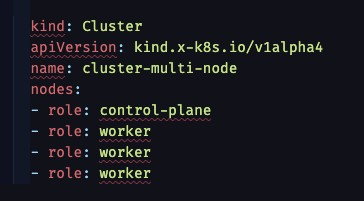
\includegraphics[width=1\textwidth]{resources/appendix/pembuatan-cluster.jpg}
  \caption{Konfigurasi Pembuatan \textit{Kubernetes Cluster} dengan \textit{Kind}}
  \label{fig:konfigurasi-pembuatan-cluster}
\end{figure}

\begin{figure}[ht]
  \centering
  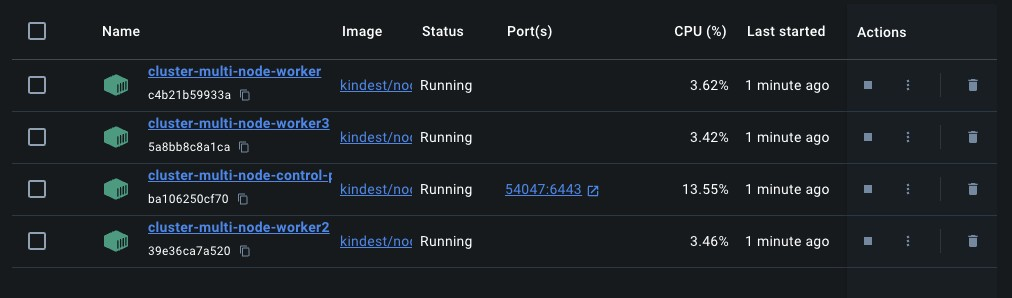
\includegraphics[width=1\textwidth]{resources/chapter-4/cluster-kind.jpg}
  \caption{Hasil \textit{Kubernetes Cluster} Dengan Kakas \textit{Kind}}
  \label{fig:hasil-cluster-kind}
\end{figure}

\pagebreak

\subsection{Implementasi \textit{Dashboard}}
Komponen \textit{dashboard} dibuat dengan menggunakan bahasa pemrogramman \textit{typescript} dan \textit{vue}. Framework yang digunakan dalam membuat \textit{Dashboard} adalah \textit{Nuxt}. \textit{Nuxt} menjadi pilihan karena memiliki \textit{developer experience} yang bagus serta fitur yang cukup lengkap. \textit{Nuxt} juga memiliki \textit{UI library} yaitu \textit{NuxtUI} yang memudahkan pembuatan \textit{UI}. Pada komponen ini, terdapat 10 halaman yang dapat dikunjungi oleh \textit{user}. Detail dari penjelasan setiap halaman dapat ditemukan pada subbab dibawah ini.

\subsubsection{Halaman \textit{Login}}
Halaman ini berada pada \textit{route} /login. Halaman ini yang berfungsi sebagai \textit{entrypoint} dari komponen \textit{dashboard}. Pada halaman ini terdapat dua input yang di \textit{wrap} oleh sebuah \textit{form}. Input berupa \textit{email} dan \textit{password} \textit{user}. Setelah \textit{user} memasukan \textit{email} dan \textit{password} yang sesuai, maka dilakukan \textit{redirect} ke laman utama untuk menunjukan bahwa \textit{user} berhasil terautentikasi dan menggunakan fungsionalitas \textit{dashboard}. Tampilan halaman ini dapat dilihat pada lampiran \ref{fig:halaman-login}.

\subsubsection{Halaman utama}
Halaman ini merupakan halaman utama dari komponen \textit{dashboard}. Pada halaman ini \textit{user} dapat melihat status dari masing masing objek mulai dari \textit{deployment}, \textit{device}, \textit{group}, serta \textit{quick actions} untuk menuju halaman terkait.

\subsubsection{Halaman \textit{Account}}
Halaman ini berada pada \textit{route /account}. Halaman ini berfungsi untuk memberikan detail mengenai \textit{company} dari \textit{user}. Informasi \textit{company} ditampilkan pada sebuah \textit{card} yang berada pada tengah halaman. Pada halaman ini juga ditampilkan informasi mengenai daftar \textit{user} yang berada pada \textit{company} yang sama dan ditampilkan dengan sebuah tabel. Tampilan halaman ini dapat dilihat pada lampiran \ref{fig:halaman-account}.

\subsubsection{Halaman \textit{Device}}
Halaman ini berada pada \textit{route /devices}. Halaman ini berfungsi untuk melakukan manajemen \textit{device} pada satu perusahaan. Halaman ini menunjukan informasi seluruh \textit{device} yang terdaftar pada \textit{company}. Tampilan halaman ini dapat dilihat pada lampiran \ref{fig:halaman-device}.

Sama seperti halaman \textit{account}, terdapat tombol dengan icon elipsis pada bagian kanan untuk melakukan fungsi seperti melihat detail ataupun menghapus \textit{device} terkait. Apabila \textit{user} menekan tombol \textit{detail} maka user diarahkan ke halaman /device/:id sesuai dengan id \textit{device} yang dipilih. Tombol yang dimaksud dapat dilihat pada lampiran \ref{fig:halaman-device-actions}.

Pada halaman ini terdapat tombol yang dapat ditekan untuk menambahkan \textit{device}. Apabila ditekan muncul sebuah modal yang berisi input yang dapat \textit{user} isi untuk membuat sebuah \textit{device} baru pada sistem. Terdapat validasi pada setiap input, setelah semua validasi dilewati, tombol \textit{submit} mengirimkan \textit{request} ke \textit{server} untuk di proses. Tombol yang dimaksud dapat dilihat pada lampiran \ref{fig:halaman-device-add}.

Akan muncul sebuah notifikasi pada bagian kanan bawah tergantung \textit{response} yang diberikan oleh \textit{server}. Warna hijau menandakan bahwa \textit{response} sukses dan warna \textit{merah} menandakan bahwa terdapat masalah ketika memproses \textit{request}.

\subsubsection{Halaman \textit{Device detail}}
Halaman ini dapat diakses dengan cara mengunjungi /devices/:id dari tombol \textit{detail} pada \textit{actions} yang berada pada halaman /devices. Pada halaman ini \textit{user} dapat menambahkan \textit{device} ke dalam sebuah group dengan menekan tombol \textit{add group}. Halaman dapat dilhat pada lampiran \ref{fig:halaman-device-detail}.

Modal \textit{add group} muncul jika tombol ditekan, modal ini memliki sebuah dropdown yang telah berisi \textit{group} yang tersedia pada sistem. Akan muncul sebuah notifikasi pada bagian bawah kanan untuk menandakan bahwa \textit{request} berhasil di proses oleh server. Warna hijau menandakan sukses dan warna merah menandakan bawhwa \textit{server} belum berhasil memproses permintaan tersebut. Modal dapat dilhat pada lampiran \ref{fig:halaman-device-detail-add-group}.

Pada halaman ini juga terdapat tombol \textit{delete} yang berada pada pojok kanan atas. Jika \textit{user} memutuskan untuk menghapus \textit{device}, muncul sebuah modal konfirmasi sebelum aksi penghapusan dilakukan. Modal dapat dilihat pada lampiran \ref{fig:halaman-device-detail-delete}.

\subsubsection{Halaman \textit{Groups}}
Halaman ini berada pada \textit{route /groups}. Halaman ini menunjukan informasi mengenai \textit{groups} yang telah terdaftar pada sistem. Informasi ditampilkan dalam bentuk tabel yang berisi detail dari objek \textit{groups}. Halaman dapat dilihat pada lampiran \ref{fig:halaman-groups}.

Pada tabel terdapat tombol elipsis yang terletak pada bagian kanan dari masing masing \textit{row}. Sama seperti tabel lainnya, tombol ini berfungsi untuk melakukan \textit{action} pada \textit{row}. Aksi yang dapat dilakukan berupa mengakses halaman detail atau menghapus \textit{item} tersebut.

Apabila tombol \textit{detail} dipilh maka \textit{user} menuju halaman \textit{group detail}. Apabila tombol \textit{delete} dipilih maka \textit{item} dihapus dari sistem dan muncul notifikasi pada bagian bawah yang menandkana bahwa proses berhasil dilakukan. Tombol dapat dilhat pada lampiran \ref{fig:halaman-groups-actions}.

Pada halaman ini juga \textit{user} dapat menambahkan \textit{groups} dengan menekan tombol \textit{add group}. Ketika tombol ini ditekan, muncul modal yang memiliki input nama. Input ini memiliki validasi berupa panjang karakter yang dimasukan haruslah memiliki panjang minimal 8 karakter. Tombol submit berfungsi untuk mengirimkan \textit{request} ke server. Akan muncul notifikasi pada bagian bawah kanan untuk menandakan bahwa \textit{request} berhasil di proses. Warna hijau menandakan bahwa \textit{request} berhasil di proses dan warna merah menandakan sebaliknya. Modal dapat dilihat pada lampiran \ref{fig:halaman-groups-add}.

\subsubsection{Halaman \textit{Groups detail}}
Halaman ini dapat diakses oleh \textit{pengguna} melalui tombol \textit{detail} yang ada pada tabel di halaman \textit{groups}. Halaman ini memiliki \textit{route /groups/:id}. Pada halaman ini \textit{user} dapat melihat informasi mengenai detail dari \textit{groups} yang dipilih mulai dari nama, deskripsi dan \textit{device} apa saja yang telah terhubung pada \textit{group tersebut}. Halaman dapat dilihat pada lampiran \ref{fig:halaman-groups-detail}.

\textit{user} juga dapat menambahkan \textit{device} dengan cara menekan tombol \textit{add devices} yang memunculkan modal berisi dropdown seluruh perangkat yang belum memiliki \textit{groups}. \textit{Dropdown} dapat dilihat pada lampiran \ref{fig:halaman-groups-detail-add-group} dan \ref{fig:halaman-groups-detail-delete}.

\subsubsection{Halaman \textit{Deployment}}
Halaman ini merupakan fungsionalitas utama dari sistem \textit{remote deployment}. Halaman ini dapat diakses melalui \textit{sidebar} dan memiliki \textit{route /deployments}. Pada halaman ini \textit{user} dapat melihat informasi mengenai \textit{deployment plan} yang terdaftar pada sistem. Selain itu juga terdapat informasi mengenai \textit{deployment images} yang tersedia dalam sistem. Kedua informasi ditampilkan dalam bentuk tabel yang masing masing memiliki tombol \textit{add} pada bagian kanan bawah tabel. Halaman dapat dilihat pada lampiran \ref{fig:halaman-deployment}.

Tombol add tersebut memunculkan modal yang berisi input yang harus diisi jika ingin membuat \textit{item} baru. Sama seperti tabel lainnya, pada masing masing tabel terdapat tombol elipsis pada bagian kanan untuk melakukan aksi berupa melihat \textit{detail} ataupun menghapus \textit{item} yang bersesuaian. Tampilan tombol dapat dilihat pada lampiran \ref{fig:halaman-deployment-add-deployment} dan \ref{fig:halaman-deployment-add-repostory}.

\subsubsection{Halaman \textit{deployments detail}}
Halaman ini dapat diakses melalui tombol \textit{detail} di tabel \textit{deployment} pada halaman \textit{deployment}. Halaman ini memiliki \textit{route /deployments/:id}. Halaman ini menunjukan informasi mengenai \textit{deployment} yang telah dilakukan, status dari \textit{deployment}, serta target dari \textit{deployment} tersebut. Tampilan halaman dapat dilihat pada lampiran \ref{fig:halaman-deployment-detail}.

Pada halaman ini juga terdapat tombol \textit{delete} yang berada pada pojok kanan atas. Dengan menekan tombol ini muncul sebuah modal untuk melakukan konfirmasi jika ingin menghapus \textit{deployment}. Tampilan dapat dilihat pada lampiran \ref{fig:halaman-deployment-detail-delete}.

\subsubsection{Halaman \textit{FAQ}}
Halaman ini berada pada \textit{route /faq}. Halaman ini bertujuan untuk memberikan informasi mengenai tata cara hal yang perlu dilakukan sebelum mendaftarkan \textit{device} ke sistem. Terdapat dua bagian yang dibedakan dari banyaknya \textit{device} yang terhubung ke dalam sistem. Dua kategori tersebut yaitu jika belum memiliki \textit{device} sama sekali dan memiliki setidaknya 1 \textit{device} yang telah terhubung dengan sistem.


\subsection{Implementasi \textit{Service}}
\label{subsec:implementasi-service}

Implementasi \textit{service} dibuat dengan menggunakan bahasa pemrogramman golang dan framework \textit{Echo} serta menggunakan \textit{REST API} sebagai gaya komunikasinya. Arsitektur kode yang dibuat memiliki tiga lapisan dimulai dari \textit{handler}, \textit{usecase}, dan \textit{repository}. Handler bertujuan membaca permintaan pengguna dan dapat disebut sebagai entrypoint. Data dari handler diberikan kepada \textit{usecase} untuk diproses. \textit{Usecase} merupakan lapisan yang hanya memiliki \textit{logic} proses bisnis. Setelah data berhasil melewati lapisan \textit{usecase}, data siap untuk dimasukkan ke database. Proses hubungan antara \textit{service} dengan \textit{database} diletakan pada lapisan \textit{repository}.

Pemisahan lapisan ini mengikuti design pattern yaitu \textit{dependency injection}. Selain itu, pemisahan ini juga bertujuan memudahkan testing dan meningkatkan \textit{maintanability} karena mudah untuk dibaca dan dipahami. \textit{endpoint} dibuat dengan menggunakan versioning dengan base \textit{endpoint} /v1. Versioning digunakan untuk memudahkan penggantian endpoint jika suatu saat terdapat perubahan major yang bersifat \textit{breaking}. Selain itu base \textit{endpoint} untuk \textit{user} dan \textit{admin} memiliki perbedaan pada prefix /api dan /admin-api

Pada sistem ini terdapat \textit{middleware} yang digunakan untuk melakukan otorisasi \textit{pengguna}. Berikut merupakan daftar dan penjelasan \textit{middleware} pada sistem

\begin{enumerate}
    \item ValidateAPIKey

          \textit{Middleware} ini bertujuan untuk memastikan bahwa hanya \textit{client} yang sesuai lah yang dapat mengakses \textit{service}. API Key dikirimkan dengan cara meletakan pada header dengan key X-API-Key. Middleware ini dijalankan untuk seluruh \textit{endpoint} yang ada pada \textit{service}.

    \item ValidateJWTKey

          \textit{Middleware} ini memiliki fungsi untuk memvalidasi JWT ketika \textit{user} melakukan \textit{request}. \textit{Middleware} ini dijalankan dengan melakukan parsing \textit{accessToken} yang didapat dari cookie pada setiap \textit{request}. Cookie didapat saat \textit{user} telah melakukan login sebelumnya dan memiliki batas waktu \textit{expire}. Setelah berhasil \textit{login} \textit{user} memiliki dua buah cookie yaitu \textit{accessToken} dan \textit{refreshToken}.  \textit{Middleware} ini berjalan untuk seluruh \textit{endpoint user} kecuali \textit{refresh dan login}


    \item ValidateAdminAPIKey

          \textit{middleware} ini memiliki fungsi untuk melakukan otorisasi \textit{admin}. Terdapat Admin API Key yang dilietakan pada header dari setiap \textit{request} dengan key X-Admin-API-Key. Middleware ini berjalan untuk seluruh \textit{endpoint} dengan prefix admin-api.
\end{enumerate}


\subsubsection{Domain \textit{company}}

Domain ini memiliki 4 \textit{endpoint} dengan deskripsi 1 untuk \textit{user} dan 3 untuk \textit{admin}. \textit{middleware} ValidateJWTKey digunakan pada \textit{endpoint user}. Untuk ketiga \textit{endpoint} admin, menggunakan \textit{middleware} ValidateAdminAPIKey. Implementasi dari domain ini dijelaskan untuk setiap fungsi dengan acuan gambar \ref{fig:company-class-diagram} dan pemetaan \textit{endpoint} dapat dilihat pada tabel \ref{tab:api-contract-domain-company}


\bgroup
\begin{table}[htbp]
    \caption{Api Contract Domain Company}
    \label{tab:api-contract-domain-company}
    \def\arraystretch{1.7}
    \centering
    \begin{tabular}{|c|p{6cm}|p{4cm}|}
        \hline
        Method & Endpoint                    &
        Fungsi                                                  \\
        \hline
        GET    & /api/v1/companies           & GetCompanyDetail \\
        \hline
        POST   & /admin-api/v1/companies     & Create           \\
        \hline
        GET    & /admin-api/v1/companies     & GetAll           \\
        \hline
        GET    & /admin-api/v1/companies/:id & GetById          \\
        \hline
        DELETE & /admin-api/v1/companies/:id & Delete           \\
        \hline
    \end{tabular}
\end{table}
\egroup

\begin{enumerate}
    \item Create

          Fungsionalitas ini menerima masukan berupa json dengan \textit{field} \textit{name} dan \textit{cluster\textunderscore name} dari \textit{requester}. Kedua \textit{field} tersebut digunakan untuk mengidentifikasi cluster dari setiap \textit{company}. Terdapat validasi berupa unique (name, cluster\textunderscore name) pada \textit{databse} untuk memastikan bahwa tidak ada duplikat untuk setiap \textit{company}. Setelah semua validasi selesai \textit{server} memberikan \textit{response} berupa objek \textit{company} kepada \textit{requester}. Apabila gagal maka diberikan pesan error

    \item GetAll

          Fungsionalitas ini dapat dipanggil tanpa masukan apapun oleh admin. Fungsionalitas ini mengembalikan semua \textit{company} yang ada pada \textit{database} lalu mengembalikan kepada \textit{requester}.

    \item GetById

          Fungsionalitas ini dapat diakses oleh admin dengan cara memberikan \textit{company id} pada URL. Fungsi ini mencari id yang bersesuaian pada \textit{database} lalu mengembalikannya kepada \textit{requester}. Apabila id yang diberikan tidak valid maka dikembalikan pesan error

    \item GetCompanyDetail

          Fungsionalitas ini dapat diakses oleh \textit{user} untuk mendapatkan informasi \textit{company detail} miliknya. Fungsionalitas ini tidak menerima request apapun namun terdapat validasi jika \textit{companyId} dari \textit{user} tidak valid maka diberikan pesan error serta apabila \textit{accessToken} sudah \textit{expire} dikeluarkan pesan \textit{unauthorized}

    \item Delete

          Fungsionalitas ini dapat diakses oleh \textit{admin} untuk menghapus \textit{company} dari \textit{database}. Karena \textit{company} memiliki relasi ke banyak domain, ketika \textit{company} di delete, diadaptasi sistem \textit{cascade} sehingga seluruh data yang memiliki referensi ke \textit{companyId} terhapus secara otomatis.

\end{enumerate}


\subsubsection{Domain \textit{user}}

Domain ini memiliki relasi \textit{one} to \textit{many} dengan domain \textit{company} karena satu company bisa memiliki banyak \textit{user}. Terdapat 7 \textit{endpoint} dengan detail 4 untuk \textit{user} dan 3 untuk \textit{admin}. Implementasi dari domain ini dijelaskan untuk setiap fungsi dengan acuan gambar \ref{fig:user-class-diagram} dan pemetaan \textit{endpoint} dapat dilihat pada tabel \ref{tab:api-contract-domain-user}

\bgroup
\begin{table}[htbp]
    \caption{Api Contract Domain User}
    \label{tab:api-contract-domain-user}
    \def\arraystretch{1.7}
    \centering
    \begin{tabular}{|c|p{6cm}|p{4cm}|}
        \hline
        Method & Endpoint                &
        Fungsi                                     \\
        \hline
        GET    & /api/v1/users           & GetAll  \\
        \hline
        GET    & /api/v1/users/:id       & GetById \\
        \hline
        POST   & /api/v1/users/login     & Login   \\
        \hline
        POST   & /api/v1/users/refresh   & Refresh \\
        \hline
        GET    & /admin-api/v1/users     & GetAll  \\
        \hline
        POST   & /admin-api/v1/users     & Create  \\
        \hline
        DELETE & /admin-api/v1/users/:id & Delete  \\
        \hline
    \end{tabular}
\end{table}
\egroup

\pagebreak

\begin{enumerate}
    \item GetAll

          Fungsionalitas ini dapat dipanggil tanpa masukan apapun. Fungsi ini memiliki pengecekan apakah user ataupun admin dan mengembalikan hasil yang sesuai. Jika \textit{user} yang memanggil fungsi ini maka dikembalikan user pada satu \textit{company} dan jika \textit{admin} yang memanggil ini maka dikembalikan seluruh user yang ada kepada \textit{requester}.

    \item GetById

          Fungsionalitas ini dapat diakses oleh \textit{user} dengan cara memberikan \textit{user id} pada URL. Fungsi ini mencari id yang bersesuaian pada \textit{database} lalu mengembalikannya kepada \textit{requester}. Apabila id yang diberikan tidak valid maka dikembalikan pesan error

    \item Login

          Fungsionalitas ini menerima masukan berupa json dengan \textit{field} \textit{email} dan \textit{password} dari \textit{requester}. Kedua field tersebut digunakan untuk mencari \textit{user} yang bersesuaian pada \textit{database}. Setelah data ditemukan dilakukan validasi password dengan cara melakukan \textit{compare hash} password dengan hash password yang tersimpan di \textit{database}. Setelah semua validasi berhasil dilakukan maka dikembalikan response serta cookie dengan "accessToken" dan "refreshToken". Apabila gagal maka diberikan pesan error

          Kedua cookie ini digunakan untuk mengotorisasi setiap request. "accessToken" memiliki waktu \textit{expire} selama 1 jam dan "refreshToken" memiliki waktu \textit{expire} selama 1 hari. Untuk meningkatkan keamanan dan menghindari CSRF, Cookie di set dengan attribut "httpOnly", "sameSiteLax", serta "secure".

    \item Refresh

          Fungsionalitas ini menerima masukan berupa "refreshToken" dan memberikan "accessToken" baru ketika \textit{endpoint} ini di panggil oleh \textit{requester}. "refreshToken" \textit{expire} secara otomatis setelah 1 hari sehingga \textit{endpoint} ini otomatis mengembalikan pesan error jika "refreshToken" sudah \textit{expire}.

    \item Create

          Fungsionalitas ini menerima masukan berupa json dengan \textit{field} \textit{name}, \textit{email}, \textit{password}, serta \textit{company\textunderscore id} dari \textit{requester}. Seluruh \textit{field} tersebut digunakan untuk membuat objek user pada \textit{database}. Pada fungsi ini dilakukan pengecekan apakah \textit{email} valid dan \textit{unique}. Selain itu ada validasi \textit{company\textunderscore id} agar dipastikan bahwa \textit{user} benar terdaftar ke \textit{company} yang sesuai. Apabila validasi tidak berhasil maka dikeluarkan pesan error, namun jika semua berhasil dilewati maka dikembalikan \textit{response} berupa \textit{user} yang telah dibuat pada \textit{database}.

    \item Delete

          Fungsionalitas ini dapat diakses oleh \textit{admin} untuk menghapus \textit{user} dari \textit{database}. Fungsi ini menerima parameter berupa id dari \textit{user} yang ingin dihapus. Apabila ada \textit{relasi} lain yang mengacu kepada \textit{user}, maka diadaptasi sistem \textit{cascade} sehingga seluruh data ikut terhapus.

\end{enumerate}

\subsubsection{Domain \textit{devices}}

Domain ini memiliki relasi \textit{one} to \textit{many} dengan domain \textit{company} karena satu company bisa memiliki banyak \textit{devices}. Terdapat 6 \textit{endpoint} dengan detail 5 untuk \textit{user} dan 1 untuk \textit{admin}. Implementasi domain ini dijelaskan untuk setiap fungsi dengan acuan gambar \ref{fig:device-class-diagram} dan pemetaan \textit{endpoint} dapat dilihat pada tabel \ref{tab:api-contract-domain-device}

\bgroup
\begin{table}[htbp]
    \caption{Api Contract Domain Devices}
    \label{tab:api-contract-domain-device}
    \def\arraystretch{1.7}
    \centering
    \begin{tabular}{|c|p{6cm}|p{4cm}|}
        \hline
        Method & Endpoint                   &
        Fungsi                                                    \\
        \hline
        GET    & /admin-api/v1/devices      & GetAll              \\
        \hline
        GET    & /api/v1/devices            & GetAllByCompanyId   \\
        \hline
        GET    & /api/v1/devices/:id        & GetById             \\
        \hline
        GET    & /api/v1/devices/:id/groups & GetGroupsByDeviceId \\
        \hline
        POST   & /api/v1/devices            & Create              \\
        \hline
        DELETE & /api/v1/devices/:id        & Delete              \\
        \hline
    \end{tabular}
\end{table}
\egroup

\pagebreak

\begin{enumerate}
    \item GetAll

          Fungsionalitas ini dapat dipanggil tanpa masukan apapun. Fungsi ini digunakan untuk admin untuk mendapatkan seluruh informasi \textit{device} yang terdaftar pada \textit{database}. Tidak ada validasi dan apabila data kosong maka dikembalikan daftar kosong.

    \item GetAllByCompanyId

          Fungsionalitas ini dapat diakses oleh \textit{user} untuk mendapatkan seluruh \textit{device} yang dimiliki oleh \textit{company}. Middleware ValidateJWTKey  melakukan \textit{decode} "accessToken" dan mengambil informasi "companyId" dari hasil tersebut. Jika tidak valid maka dikeluarkan pesan error. Setelah semua validasi berhasil maka daftar seluruh \textit{device} menjadi \textit{repsonse} dan dikembalikan kepada \textit{requester}.

    \item GetById

          Fungsionalitas ini dapat diakses oleh \textit{user} untuk mendapatkan detail dari \textit{device} dengan cara memberikan \textit{id} yang sesuai. Apabila tidak ditemukan maka dikeluarkan pesan error.

    \item GetGroupsByDeviceId


          Fungsionalitas ini mengembalikan seluruh relasi \textit{groups} yang berkaitan dengan \textit{device id} terkait. Fungsi ini menerima \textit{device id} dan mencari apakah terdapat \textit{groups} yang berkaitan dengan id tersebut. Fungsi ini mengembalikan seluruh \textit{groups} yang ada dan jika tidak ada satupun maka dikeluarkan daftar kosong. Apabila \textit{device id} tidak valid maka diberikan pesan error.

    \item Create

          Fungsionalitas ini menerima masukan berupa json dengan \textit{field} \textit{name}, \textit{type}, \textit{attributes}, serta \textit{node\textunderscore name} dari \textit{requester}. Seluruh \textit{field} tersebut digunakan untuk membuat objek \textit{device} pada \textit{database}. Pada fungsi ini dilakukan pengecekan apakah \textit{node\textunderscore name} ada pada \textit{cluster} serta merupakan nama yang valid dan \textit{unique}. Selain itu terdapat validasi \textit{attributes} yaitu merupakan list of string yang masing masing harus memiliki '=' sebagai tanda pemisah. Hal ini dilakukan karena ini merupakan label yang diberikan pada \textit{node} pada \textit{cluster} nantinya. Apabila validasi tidak berhasil maka dikeluarkan pesan error, namun jika semua berhasil dilewati maka dikembalikan \textit{response} berupa \textit{device} yang telah dibuat pada \textit{database} serta proses \textit{node} pada \textit{cluster} yang sudah di labeli dengan \textit{attributes}.

    \item Delete

          Fungsionalitas ini dapat diakses oleh \textit{user} untuk menghapus \textit{device} dari \textit{database}. Fungsi ini menerima parameter berupa id dari \textit{device} yang ingin dihapus. Apabila ada \textit{relasi} lain yang mengacu kepada \textit{device}, maka diadaptasi sistem \textit{cascade} sehingga seluruh data ikut terhapus.

\end{enumerate}

\subsubsection{Domain \textit{groups}}

Domain ini memiliki relasi \textit{one} to \textit{many} dengan domain \textit{company} karena satu \textit{company} bisa memiliki banyak \textit{groups}. Terdapat 6 \textit{endpoint} dengan detail 5 untuk \textit{user} dan 1 untuk \textit{admin}. Implementasi dari domain ini dijelaskan untuk setiap fungsi dengan acuan gambar \ref{fig:groups-class-diagram} dan pemetaan \textit{endpoint} dapat dilihat pada tabel \ref{tab:api-contract-domain-groups}

\bgroup
\begin{table}[htbp]
    \caption{Api Contract Domain Groups}
    \label{tab:api-contract-domain-groups}
    \def\arraystretch{1.7}
    \centering
    \begin{tabular}{|c|p{6cm}|p{4cm}|}
        \hline
        Method & Endpoint                  &
        Fungsi                                                  \\
        \hline
        GET    & /admin-api/v1/groups      & GetAll             \\
        \hline
        GET    & /api/v1/groups            & GetAllByCompanyId  \\
        \hline
        GET    & /api/v1/groups/:id        & GetById            \\
        \hline
        GET    & /api/v1/groups/:id/groups & GetDeviceByGroupId \\
        \hline
        POST   & /api/v1/groups            & Create             \\
        \hline
        DELETE & /api/v1/groups/:id        & Delete             \\
        \hline
    \end{tabular}
\end{table}
\egroup

\pagebreak

\begin{enumerate}
    \item GetAll

          Fungsionalitas ini dapat dipanggil tanpa masukan apapun. Fungsi ini digunakan untuk admin untuk mendapatkan seluruh informasi \textit{groups} yang terdaftar pada \textit{database}. Tidak ada validasi dan apabila data kosong maka dikembalikan daftar kosong.

    \item GetAllByCompanyId

          Fungsionalitas ini dapat diakses oleh \textit{user} untuk mendapatkan seluruh \textit{groups} yang dimiliki oleh \textit{company}. Middleware ValidateJWTKey  melakukan \textit{decode} "accessToken" dan mengambil informasi "companyId" dari hasil tersebut. Jika tidak valid maka dikeluarkan pesan error. Setelah semua validasi berhasil maka daftar seluruh \textit{groups} menjadi \textit{repsonse} dan dikembalikan kepada \textit{requester}.

    \item GetById

          Fungsionalitas ini dapat diakses oleh \textit{user} untuk mendapatkan detail dari \textit{groups} dengan cara memberikan \textit{id} yang sesuai. Apabila tidak ditemukan maka dikeluarkan pesan error.

    \item GetDeviceByGroupId


          Fungsionalitas ini mengembalikan seluruh relasi \textit{device} yang berkaitan dengan \textit{group id} terkait. Fungsi ini menerima \textit{group id} dan mencari apakah terdapat \textit{device} yang berkaitan dengan id tersebut. Fungsi ini mengembalikan seluruh \textit{device} yang ada dan jika tidak ada satupun maka dikeluarkan daftar kosong. Apabila \textit{group id} tidak valid maka diberikan pesan error.

    \item Create

          Fungsionalitas ini menerima masukan berupa json dengan \textit{field} \textit{name}. \textit{Field name} memiliki \textit{unique constraint} sehingga tidak mungkin ada nama \textit{groups} yang sama pada satu \textit{company}. Terdapat validasi untuk membuat nama \textit{groups} yang memiliki panjang minimal 8 characters untuk menghindari memberikan nama tanpa konteks. Apabila terdapat duplikat dikembalikan pesan error dan setelah semua validasi berhasil, \textit{service} mengirimkan \textit{response} berupa \textit{groups} yang berhasil dibuat kepada \textit{requester}.

    \item Delete

          Fungsionalitas ini dapat diakses oleh \textit{user} untuk menghapus \textit{groups} dari \textit{database}. Fungsi ini menerima parameter berupa id dari \textit{groups} yang ingin dihapus. Apabila ada \textit{relasi} lain yang mengacu kepada \textit{groups}, maka diadaptasi sistem \textit{cascade} sehingga seluruh data ikut terhapus.

\end{enumerate}


\subsubsection{Domain \textit{deployment}}

Domain ini memiliki relasi \textit{one} to \textit{one} dengan domain \textit{external service}. Selain itu domain ini juga memiliki relasi one to many dengan \textit{company}. Karena satu \textit{company} bisa memiliki banyak \textit{deployment}. Pada domain ini dibagi menjadi tiga bagian yaitu \textit{deployment images}, \textit{deployment histories} dan \textit{deployment}. Hubungan domain dapat dilihat pada gambar \ref{fig:deployment-class-diagram}

\subsubsubsection{Deployment Images}
Pada bagian ini yang terdapat 5 \textit{endpoint} dengan detail 4 untuk \textit{user} dan 1 untuk \textit{admin}. Implementasi dari domain ini dijelaskan untuk setiap fungsi dengan acuan gambar \ref{fig:deployment-class-diagram} dan pemetaan \textit{endpoint} dapat dilihat pada tabel \ref{tab:api-contract-domain-deployment-images}

\bgroup
\begin{table}[htbp]
    \caption{Api Contract Domain Deployment Images}
    \label{tab:api-contract-domain-deployment-images}
    \def\arraystretch{1.7}
    \centering
    \begin{tabular}{|c|p{6cm}|p{4cm}|}
        \hline
        Method & Endpoint                   &
        Fungsi                                                  \\
        \hline
        GET    & /admin-api/v1/repositories & GetAll            \\
        \hline
        GET    & /api/v1/repositories       & GetAllByCompanyId \\
        \hline
        GET    & /api/v1/repositories/:id   & GetById           \\
        \hline
        POST   & /api/v1/repositories       & Create            \\
        \hline
        DELETE & /api/v1/repositories/:id   & Delete            \\
        \hline
    \end{tabular}
\end{table}
\egroup

\pagebreak

\begin{enumerate}
    \item GetAll

          Fungsionalitas ini dapat dipanggil tanpa masukan apapun. Fungsi ini digunakan untuk admin untuk mendapatkan seluruh informasi \textit{deployment images} yang terdaftar pada \textit{database}. Tidak ada validasi dan apabila data kosong maka dikembalikan daftar kosong.

    \item GetAllByCompanyId

          Fungsionalitas ini dapat diakses oleh \textit{user} untuk mendapatkan seluruh \textit{deployment images} yang dimiliki oleh \textit{company}. Middleware ValidateJWTKey  melakukan \textit{decode} "accessToken" dan mengambil informasi "companyId" dari hasil tersebut. Jika tidak valid maka dikeluarkan pesan error. Setelah semua validasi berhasil maka daftar seluruh \textit{deployment images} menjadi \textit{repsonse} dan dikembalikan kepada \textit{requester}.

    \item GetById

          Fungsionalitas ini dapat diakses oleh \textit{user} untuk mendapatkan detail dari \textit{deployment images} dengan cara memberikan \textit{id} yang sesuai. Apabila tidak ditemukan maka dikeluarkan pesan error.

    \item Create

          Fungsionalitas ini menerima masukan berupa json dengan \textit{field} \textit{name}, \textit{description}, \textit{image}. Teradapat \textit{unique constraint} pada \textit{field nama dan image} pada satu \textit{company} untuk mencegah duplikat. Apabila terdapat duplikat maka dikembalikan pesan error dan setelah semua validasi berhasil, \textit{service} mengirimkan \textit{response} berupa \textit{deployment images} yang berhasil dibuat kepada \textit{requester}.

    \item Delete

          Fungsionalitas ini dapat diakses oleh \textit{user} untuk menghapus \textit{eployment images} dari \textit{database}. Fungsi ini menerima parameter berupa id dari \textit{eployment images} yang ingin dihapus. Apabila ada \textit{relasi} lain yang mengacu kepada \textit{eployment images}, maka diadaptasi sistem \textit{cascade} sehingga seluruh data ikut terhapus.

\end{enumerate}

\subsubsubsection{Deployment Histories}
Pada bagian ini yang terdapat 5 \textit{endpoint} dengan detail 4 untuk \textit{user} dan 1 untuk \textit{admin}. Implementasi dari domain ini dijelaskan untuk setiap fungsi dengan acuan gambar \ref{fig:deployment-class-diagram} dan pemetaan \textit{endpoint} dapat dilihat pada tabel \ref{tab:api-contract-domain-deployment-histories}

\bgroup
\begin{table}[htbp]
    \caption{Api Contract Domain Deployment Histories}
    \label{tab:api-contract-domain-deployment-histories}
    \def\arraystretch{1.7}
    \centering
    \begin{tabular}{|c|p{6cm}|p{4cm}|}
        \hline
        Method & Endpoint                &
        Fungsi                                               \\
        \hline
        GET    & /admin-api/v1/histories & GetAll            \\
        \hline
        GET    & /api/v1/histories       & GetAllByCompanyId \\
        \hline
        GET    & /api/v1/histories/:id   & GetById           \\
        \hline
        POST   & /api/v1/histories       & Create            \\
        \hline
        DELETE & /api/v1/histories/:id   & Delete            \\
        \hline
    \end{tabular}
\end{table}
\egroup


\begin{enumerate}
    \item GetAll

          Fungsionalitas ini dapat dipanggil tanpa masukan apapun. Fungsi ini digunakan untuk admin untuk mendapatkan seluruh informasi \textit{deployment histories} yang terdaftar pada \textit{database}. Tidak ada validasi dan apabila data kosong maka dikembalikan daftar kosong.

    \item GetAllByCompanyId

          Fungsionalitas ini dapat diakses oleh \textit{user} untuk mendapatkan seluruh \textit{deployment histories} yang dimiliki oleh \textit{company}. Middleware ValidateJWTKey melakukan \textit{decode} "accessToken" dan mengambil informasi "companyId" dari hasil tersebut. Jika tidak valid maka dikeluarkan pesan error. Setelah semua validasi berhasil maka daftar seluruh \textit{deployment histories} menjadi \textit{repsonse} dan dikembalikan kepada \textit{requester}.

    \item GetById

          Fungsionalitas ini dapat diakses oleh \textit{user} untuk mendapatkan detail dari \textit{deployment histories} dengan cara memberikan \textit{id} yang sesuai. Apabila tidak ditemukan maka dikeluarkan pesan error.

    \item Create

          Fungsionalitas ini menerima masukan berupa json dengan \textit{field} \textit{device\textunderscore id}, \textit{repository\textunderscore id}, \textit{deployment\textunderscore id}. Tidak ada validasi ketika ingin membuat \textit{deployement histories} dan \textit{Service} mengirimkan \textit{response} berupa \textit{deployment histories} yang berhasil dibuat kepada \textit{requester}.

    \item Delete

          Fungsionalitas ini dapat diakses oleh \textit{user} untuk menghapus \textit{eployment histories} dari \textit{database}. Fungsi ini menerima parameter berupa id dari \textit{deployment histories} yang ingin dihapus. Apabila ada \textit{relasi} lain yang mengacu kepada \textit{deployment histories}, diadaptasi sistem \textit{cascade} sehingga seluruh data ikut terhapus.

\end{enumerate}

\subsubsubsection{Deployment plan}
Pada bagian ini yang terdapat 7 \textit{endpoint} dengan detail 6 untuk \textit{user} dan 1 untuk \textit{admin}. Implementasi ini merupakan implementasi utama dari domain ini. Bagian ini juga menjadi terhubung dengan dua bagian lainnya serperti pada gambar \ref{fig:deployment-class-diagram}. Pemetaan \textit{endpoint} dapat dilihat pada tabel \ref{tab:api-contract-domain-deployment}

\bgroup
\begin{table}[htbp]
    \caption{Api Contract Domain Deployment plan}
    \label{tab:api-contract-domain-deployment}
    \def\arraystretch{1.7}
    \centering
    \begin{tabular}{|c|p{6cm}|p{4cm}|}
        \hline
        Method & Endpoint                          &
        Fungsi                                                         \\
        \hline
        GET    & /admin-api/v1/deployments         & GetAll            \\
        \hline
        GET    & /api/v1/deployments               & GetAllByCompanyId \\
        \hline
        GET    & /api/v1/deployments/:id           & GetById           \\
        \hline
        POST   & /api/v1/deployments               & Create            \\
        \hline
        DELETE & /api/v1/deployments/:id           & Delete            \\
        \hline
        POST   & /api/v1/deployments/deploy        & Deploy            \\
        \hline
        POST   & /api/v1/deployments/deploy/delete & DeleteDeploy      \\
        \hline
    \end{tabular}
\end{table}
\egroup

\pagebreak

\begin{enumerate}
    \item GetAll

          Fungsionalitas ini dapat dipanggil tanpa masukan apapun. Fungsi ini digunakan untuk admin untuk mendapatkan seluruh informasi \textit{deployment plan} yang terdaftar pada \textit{database}. Tidak ada validasi dan apabila data kosong maka dikembalikan daftar kosong.

    \item GetAllByCompanyId

          Fungsionalitas ini dapat diakses oleh \textit{user} untuk mendapatkan seluruh \textit{deployment plan} yang dimiliki oleh \textit{company}. Middleware ValidateJWTKey melakukan \textit{decode} "accessToken" dan mengambil informasi "companyId" dari hasil tersebut. Jika tidak valid maka dikeluarkan pesan error. Setelah semua validasi berhasil maka daftar seluruh \textit{deployment plan} menjadi hasil \textit{repsonse} untuk \textit{requester}.

    \item GetById

          Fungsionalitas ini dapat diakses oleh \textit{user} untuk mendapatkan detail dari \textit{deployment plan} dengan cara memberikan \textit{id} yang sesuai. Apabila tidak ditemukan maka dikeluarkan pesan error.

    \item Create

          Fungsionalitas ini menerima masukan berupa json dengan \textit{field} \textit{name}, \textit{version}, \textit{target}, dan \textit{repository\textunderscore id}. Terdapat validasi yaitu \textit{unique constraint} pada \textit{name, version, dan repository\textunderscore id} pada satu company yang sama untuk mencegah data duplikat yang membingungkan. Setelah validasi selsai maka \textit{Service} mengirimkan \textit{response} berupa \textit{deployment plan} yang berhasil dibuat kepada \textit{requester}. Apabila gagal maka dikirimkan pesan error.

    \item Delete

          Fungsionalitas ini dapat diakses oleh \textit{user} untuk menghapus \textit{deployment plan} dari \textit{database}. Fungsi ini menerima parameter berupa id dari \textit{deployment plan} yang ingin dihapus. Apabila ada \textit{relasi} lain yang mengacu kepada \textit{deployment plan}, diadaptasi sistem \textit{cascade} sehingga seluruh data ikut terhapus juga.

    \item Deploy

          Fungsionalitas ini merupakan fungsionalitas utama dalam sistem \textit{remote deployment}. Fungsionalitas ini dapat diakses oleh \textit{user} untuk melakukan \textit{remote deployment} sesuai dengan \textit{deployment plan} yang dipilih. Fungsi ini menerima \textit{argument} berupa daftar dari \textit{deployment plan} yang ingin dipilh. Apabila terdapat salah satu \textit{deployment plan} yang tidak ditemukan maka proses gagal. Setelah semua validasi berhasil dilakukan, fungsi ini melanjutkan untuk memanggil \textit{extenral service kubernetes controller} dengan data yang telah disesuaikan.

    \item DeleteDeploy

          Fungsionalitas ini dapat diakses oleh \textit{user} untuk melakukan \textit{rollback deployment} dari \textit{deployment plan} yang dipilih. Fungsi ini menerima \textit{argument} berupa daftar dari \textit{deployment plan} yang ingin dihapus atau dilakukan \textit{rollback}. Apabila terdapat salah satu \textit{deployment plan} yang tidak ditemukan maka proses memunculkan pesan \textit{error}

\end{enumerate}

\subsubsection{Domain \textit{external services}}

Domain ini memiliki relasi \textit{one} to \textit{one} dengan domain \textit{deployment}. Pada \textit{domain} ini tidak terdapat endpoint karena seluruh \textit{Fungsionalitas} ini digunakan pada domain \textit{deployment} pada lapisan \textit{usecase}. Implementasi dari domain ini dijelaskan untuk setiap fungsi dengan acuan gambar \ref{fig:kubernetes-controller-class-diagram}.

\pagebreak

\begin{enumerate}
    \item GetConfig

          Fungsionalitas ini digunakan untuk mendapatkan \textit{config} dari \textit{kubernetes client} yang dipakai.

    \item GetNodes

          Fungsionalitas ini digunakan untuk mendapatkan seluruh \textit{nodes} yang ada pada \textit{cluster} yang sedang terhubung

    \item SwitchCluster

          Fungsionalitas ini digunakan untuk merubah \textit{koneksi cluster kubernetes} yang digunakan. Karena setiap \textit{company} punya \textit{cluster\textunderscore name} yang berbeda beda maka ketika terdapat \textit{company} yang berbeda yang ingin memproses \textit{deployment} maka domain ini dapat melakukan manajemen \textit{cluster} yang terhubung.

    \item LabelNode

          Fungsionalitas ini digunakan untuk membuat label pada \textit{node} di \textit{cluster}. Label haruslah berbentuk key value yang dipisahkan dengan tanda =. Apabila label tidak valid maka dimunculkan pesan \textit{error}.

    \item Deploy

          Fungsionalitas ini digunakan untuk melakukan deployment pada \textit{cluster}. Deployment dilakukan dengan menargetkan \textit{device} sesuai dengan \textit{field target} pada \textit{deployment plan}. Apabila deployment sudah pernah dibuat, maka dikeluarkan pesan error. Jika deployment belum pernah dibuat, maka proses deployment dilaksanakan dan diberikan \textit{response} berupa hasil \textit{deployment}

    \item Get

          Fungsionalitas ini digunakan untuk melakukan melihat seluruh deployment yang telah dibuat pada \textit{cluster} beserta status nya.



    \item Patch

          Fungsionalitas ini digunakan untuk \textit{mengupdate} deployment yang telah dibuat pada \textit{cluster}.

    \item Delete

          Fungsionalitas ini digunakan untuk menghapus \textit{deployment} pada \textit{cluster}.

\end{enumerate}

% \pagebreak

% \section{Pengujian}
\label{sec:pengujian}


Tujuan dari pengujian ialah untuk memastikan apakah seluruh kebutuhan fungsional dan non-fungsional dari sistem telah terpenuhi.
Untuk pengujian kebutuhan fungsional, pengujian dibagi menjadi dua bagian yaitu pengujian yang dilakukan per komponen lalu dilanjutkan dengan pengujian sistem. Setiap skenario pengujian dijelaskan tujuannya, skenario yang dilakukan, dan hasil pengujian yang didapatkan. Skenario pengujian akan memiliki ID dengan awalan P diikuti dengan dua angka. Seluruh pemetaan pengujian terdapat pada lampiran \ref{chapter:tabel-pengujian}

\subsection{Batasan Pengujian}
\label{subsec:batasan-pengujian}
Berikut adalah batasan yang ditetapkan dalam melakukan pengujian \textit{sistem remote deployment}.

\begin{enumerate}
  \item Pengujian dilakukan di tiga kluster yang berbeda
        \begin{enumerate}
          \item Kubernetes lokal \textit{cluster}
          \item \textit{Google Cloud Platform (GCP) Compute Engine} Kubernetes \textit{cluster}
          \item RaspberryPi Cluster
        \end{enumerate}
  \item Setiap \textit{cluster} memiliki jumlah node yang sama yaitu 2.
  \item \textit{Cluster} dibuat dengan distribusi kubernetes k3s.
  \item Sistem \textit{remote deployment} dijalankan pada komputer lokal yang memilki spesifikasi yang telah dijelaskan pada bagian \ref{sec:lingkungan-implementasi}.
  \item Untuk beberapa fungsionalitas admin digunakan \textit{HTTP Client} yaitu Postman untuk membuat \textit{request} kepada \textit{service}
  \item Cluster sudah tersedia dan siap diakses.
  \item Setiap \textit{request} memiliki header X-Api-Key.
  \item Setiap \textit{request} yang mengarah ke /admin-api/ memiliki \textit{header} berupa X-Admin-API-Key.
  \item \textit{Database} pada bagian "deployment images" sudah terisi sebagian untuk memudahkan proses pengujian.
\end{enumerate}

\subsection{Persiapan Pengujian}
Pada proses pengujian, terdapat tiga lingkungan pengujian yang digunakan untuk menguji sistem \textit{remote deployment}. Ketiga lingkungan tersebut yaitu kubernetes \textit{cluster} lokal, kubernetes \textit{cluster} yang terdapat di \textit{Cloud (GCP)}, serta \textit{cluster} pada RaspberryPi. Ketiga \textit{cluster} ini memiliki jumlah node yang berbeda sesuai dengan penjelasan pada \ref{subsec:batasan-pengujian}.

\subsubsection{Kubernetes Lokal}
Untuk pengujian pada kubernetes lokal, dilakukan pembuatan \textit{cluster} dengan kakas kind untuk membuat cluster yang bernama \textit{testing-cluster-two-nodes} yang memiliki 2 node. Konfigurasi pembuatan sama seperti konfigurasi pada bagian \ref{subsec:persiapan-kubernetes-cluster} hanya saja jumlah nodes yang digunakan yaitu 2.
Karena nodes berjumlah dua maka terdapat 1 \textit{master nodes} dan 1 \textit{slave} node pada \textit{cluster}. Konfigurasi pembuatan cluster dapat dilihat pada gambar \ref{fig:kubernetes-lokal-config-testing}.

\begin{figure}[htbp]
    \centering
    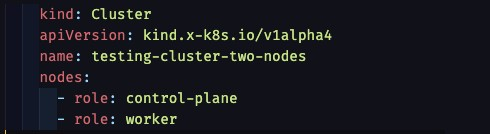
\includegraphics[width=1\textwidth]{resources/chapter-4/pengujian/kubernetes-lokal-config.jpg}
    \caption{Konfigurasi Pembuatan \textit{Kubernetes Testing Cluster} Dengan Kakas \textit{Kind}}
    \label{fig:kubernetes-lokal-config-testing}
\end{figure}

Setelah itu jalankan perintah "kind create cluster --config testing-cluster.yaml" untuk membuat \textit{cluster} pada \textit{docker}. Hasil dari perintahh ini yaitu tercipta dua buah \textit{container} pada \textit{docker} yang memiliki peran \textit{master} dan \textit{slave} seperti pada gambar \ref{fig:kubernetes-lokal-config-testing-result}.

\begin{figure}[htbp]
    \centering
    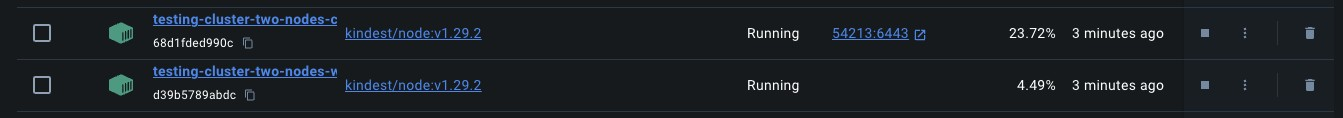
\includegraphics[width=1\textwidth]{resources/chapter-4/pengujian/kubernetes-lokal-config-result.jpg}
    \caption{Hasil \textit{Kubernetes Testing Cluster} pada \textit{Docker}}
    \label{fig:kubernetes-lokal-config-testing-result}
\end{figure}

\subsubsection{Kubernetes GCP}
\label{subsubsec:kubernetes-gcp}
Pada lingkungan ini dibuat dua buah \textit{compute engine (virtual machine)} pada \textit{GCP}. Masing masing dari \textit{virtual machine} berperan sebagai kubernetes \textit{cluster} yang bernama \textit{prod-cluster-example}.

\begin{enumerate}
    \item Buat dua \textit{virtual machine} pada \textit{compute engine GCP} dengan spesifikasi berikut. Hasil pembuatan \textit{virtual machine} dapat dilihat pada lampiran \ref{fig:hasil-pembuatan-virtual-machine-gcp}
          \begin{enumerate}
              \item Ubuntu 24.04
              \item 2GB Memory
              \item 10GB Storage Persistent Disk
              \item 0.5 - 2Vcpu (1 shared core)
              \item Region Asia southeast2-c
          \end{enumerate}
    \item Membuat \textit{Firewall Rule} Untuk membuka port yang digunakan oleh Kubernetes. Untuk daftar opsi setiap port yang dibuka dapat dilihat pada lampiran \ref{fig:daftar-kegunaan-port}. Untuk hasil pembuatan firewall dapat dilihat pada lampiran \ref{fig:hasil-firewall-rule-pada-gcp}
    \item Konfigurasi \textit{gare-test-kubernetes-server} sebagai master nodes. Konfigurasi dilakukan dengan cara mengunduh instalasi dari k3s dengan perintah seperti pada lampiran \ref{fig:instalasi-master-node-gcp}.
    \item Konfigurasi virutal machine lainnya yaitu \textit{gare-test-kubernetes-server-node} sebagai \textit{worker node}. Untuk meregistrasi \textit{node} ke dalam \textit{cluster} perlu adanya autentikasi untuk memasitikan hanya \textit{node} yang benar yang boleh masuk ke dalam \textit{cluster}. K3s memiliki token generator yang dapat digunakan untuk mencegah akses yang tidak diinginkan, registrasi token dapat dilihat pada lampiran \ref{fig:pengambilan-token-registrasi-cluster}. Token tersebut digunakan untuk meregistrasi \textit{node} ini ke \textit{master} dengan \textit{public ip} node tersebut. Ilustrasi dapat dilihat pada lampiran \ref{fig:instalasi-worker-node-gcp}.
    \item Ambil konfigurasi \textit{cluster} di \textit{master node} dan pindahkan ke lokasi \textit{server berjalan} untuk meregistrasi \textit{cluster} ke dalam sistem. Setelah melakukan kelima langkah ini \textit{cluster} sudah terintegrasi dengan sistem. Ilustrasi pemindahan konfigurasi dapat dilihat pada lampiran \ref{fig:konfigurasi-cluster-master-node-gcp} dan \ref{fig:proses-pemindahan-konfigurasi-master-gcp}.
\end{enumerate}

\subsubsection{Kubernetes RaspberryPi}
Pada lingkungan ini dibuat cluster dengan dua nodes pada RaspberryPi. Cluster yang dibuat bernama cluster-raspi yang memiliki spesifikasi hardware RaspberryPi berikut.

\begin{enumerate}
    \item Master node menggunakan Raspberry Pi 3 Model B Rev 1.2 dengan 1GB RAM dan 4 CPU @ 1.2GHz dengan hostname masterpi. Informasi lebih lengkap dapat dilihat pada lampiran \ref{fig:hostname-raspi-master-nodes} dan \ref{fig:spesifikasi-raspi-master-nodes}
    \item Worker node menggunakan Raspberry Pi 2 Model B Rev 1.1 dengan 1GB RAM dan 4 CPU @ 900MHz dengan hostname raspberrypi. Informasi lebih lengkap dapat dilihat pada lampiran \ref{fig:hostname-raspi-worker-nodes} dan \ref{fig:spesifikasi-raspi-worker-nodes}
\end{enumerate}

Berikut merupakan tata cara pembuatan cluster kubernetes pada \textit{RaspberryPi}. Diasumsikan \textit{device} \textit{RaspberryPi} sudah terhubung ke dalam jaringan yang sama sehingga tidak perlu \textit{port forwarding} / \textit{public ip}.

\begin{enumerate}
    \item Konfigurasi \textit{hostname masterpi} sebagai master nodes. Perlu dilakukan konfigurasi tambahan untuk menambahkan cgroups pada raspberrypi karena secara default opsi ini \textit{disabled}. cgroups merupakan kepanjangan dari \textit{Control Groups} yang berfungsi sebagai \textit{resource management} pada linux dan digunakan dalam proses kontainerisasi. Selanjutnya mirip serperti konfigurasi pada bagian \ref{subsubsec:kubernetes-gcp}, perlu mengunduh instalasi dari k3s dengan perintah seperti pada lampiran \ref{fig:instalasi-master-raspi-nodes}.
    \item Konfigurasi \textit{node} lainnya yaitu \textit{hostname raspberrypi} sebagai \textit{worker node}. Untuk meregistrasi \textit{node} ke dalam \textit{cluster} perlu adanya autentikasi untuk memasitikan hanya \textit{node} yang benar yang boleh masuk ke dalam \textit{cluster}. K3s memiliki token generator yang dapat digunakan untuk mencegah akses yang tidak diinginkan, registrasi token dapat dilihat pada lampiran \ref{fig:raspi-master-gen-token}. Token tersebut digunakan untuk meregistrasi \textit{node} ini ke \textit{master} dengan \textit{ip local} node master. Ilustrasi dapat dilihat pada lampiran \ref{fig:instalasi-worker-raspi-node}.
    \item Ambil konfigurasi \textit{cluster} di \textit{master node} dan pindahkan ke lokasi \textit{server berjalan} untuk meregistrasi \textit{cluster} ke dalam sistem. Setelah melakukan langkah ini \textit{cluster} sudah terintegrasi dengan sistem. Ilustrasi pemindahan konfigurasi dapat dilihat pada lampiran \ref{fig:raspi-kube-config} dan \ref{fig:raspi-add-kubeconfig}.
\end{enumerate}

\subsection{Pengujian Komponen}
Pengujian di level komponen memastikan bahwa seluruh fungsionalitas yang tidak melibatkan servis eksternal di dalam komponen bekerja dengan baik. Pengujian ini dibagi menjadi beberapa bagian sesuai dengan domain yang telah dijelaskan pada bagian \ref{subsec:implementasi-service}. Pada masing masing domain terdapat tabel yang memetakan hubungan antara kebutuhan fungsional serta pengujian yang bersesuaian. Pengujian dilakukan menggunakan lingkungan lokal dengan nama cluster "kind-testing-cluster-two-nodes"

\input{chapters/chapter-4/pengujian/02-01-domain-company.tex}
\input{chapters/chapter-4/pengujian/02-02-domain-user.tex}
\input{chapters/chapter-4/pengujian/02-03-domain-devices.tex}
\input{chapters/chapter-4/pengujian/02-04-domain-groups.tex}

\subsection{Pengujian Sistem}
Pengujian sistem memiliki kaitan dengan satu atau lebih domain dan fungsionalitas. Pengujian ini dibagi menjadi dua bagian yaitu pengujian pada \textit{cluster GCP} serta pengujian pada \textit{cluster RaspberryPi} yang dibagi berdasarkan abstrasksi kebutuhan utama yaitu melakukan \textit{remote deployment}.


\input{chapters/chapter-4/pengujian/03-01-pengujian-sistem-raspi.tex}
\input{chapters/chapter-4/pengujian/03-02-pengujian-sistem-gcp.tex}

\input{chapters/chapter-4/pengujian/03-03-pengujian-deployment-gagal.tex}

\subsection{Pengujian Non Fungsional}
Pada bagian ini, dilakukan pengujian terhadap kebutuhan non-fungsional sistem. Terdapat dua kebutuhan non-fungsional yang akan diuji yaitu \textit{Security dan Portability}. Pengujian akan menggunakan \textit{security testing} dan \textit{compatibility testing} untuk masing masing kebutuhan non-fungsional.

\subsubsection{\textit{Security Testing}}
\textit{Security Testing} bertujuan untuk menguji kebutuhan non-fungsional yaitu \textit{security}. Pengujian ini hanya terbatas pada masalah autentikasi dan authorisasi. Pengujian kebutuhan non-fungsional ini dilakukan dengan cara mencoba mengakses \textit{dashboard} dan \textit{service} tanpa meletakan token yang valid. Pengujian ini mencakup ID pengujian P47 hingga P50

\begin{enumerate}
  \item Mengakses \textit{dashboard} tanpa kredensial

        Ketika mengakses \textit{dashboard} tanpa memiliki kredensial, \textit{dashboard} memiliki \textit{middleware} yang akan mengecek token yang disimpan pada \textit{client}. Jika token tidak valid maka sistem akan langsung melakukan \textit{redirect} ke halaman login.

  \item Mengakses user \textit{service} tanpa kredensial

        Ketika mencoba untuk mengakses \textit{service} pada endpoint apapun, \textit{service} memiliki \textit{middleware}
        yang akan mengecek header authentikasi yang dikirimkan oleh client. Jika kredensial pada header tidak dicantumkan maka akan mengembalikan \textit{401 Unauthorized} seperti pada lampiran \ref{fig:akses-service-user}.

  \item Mengakses admin \textit{service} tanpa kredensial

        Admin endpoint memiliki \textit{middleware} validateAdminJWTKey. Ketika mencoba untuk mengakses \textit{endpoint} admin tanpa memberikan header X-Admin-Api-Key yang sesuai maka \textit{service} akan mengembalikan \textit{401 Unauthorized} seperti pada lampiran \ref{fig:akses-service-admin}.

  \item Mengakses \textit{url kubernetes} tanpa kredensial

        Seluruh cluster kubernetes akan mengexpose endpoint pada port 6443. Pengujian ini akan mengakses url kubernetes yaitu https://34.101.95.240:6443/. Ketika diakses, hasilnya akan menunjukan status \textit{401 Unauthorized} seperti pada lampiran \ref{fig:akses-service-kubernetes}.

\end{enumerate}

Setelah melakukan pengujian, pengujian dengan ID P47 hingga P50 berjalan sesuai dengan ekspektasi yaitu menunjukan kegagalan saat mengakses \textit{resource} yang diminta. Seluruh rekap pengujian dapat dilihat pada tabel \ref{tab:pengujian-nonfungsional-security}.

\subsubsection{Compatibility Testing}
\textit{Compatibility testing} dilakukan untuk menguji kebutuhan non-fungsional yaitu \textit{portability}. Pengujian kebutuhan non-fungsional ini dialkukan dengan tiga skenario yaitu mengakses \textit{dashboard} dari mobile serta mengakses dari berbagai \textit{browser}. Tujuan dari pengujian ini adalah memastikan bahwa \textit{dashboard} dapat dijalankan pada berbagai \textit{platform}. Pengujian ini mencakup pengujian dengan ID P52 hingga P54.

\begin{enumerate}
  \item Mengakses \textit{dashboard} dari perangkat mobile

        \textit{Dashboard} berhasil diakses melalui perangkat mobile dan dapat dilihat hasil dapat dilihat pada lampiran \ref{fig:akses-dashboard-mobile}.

  \item Mengakses \textit{dashboard} dari Chromium based browser

        \textit{Dashboard} berhasil diakses melalui browser \textit{chromium based} yaitu "Arc" dan "Google Chrome" yang dapat dilhat pada lampiran \ref{fig:akses-dashboard-chromium}.

  \item Mengakses \textit{dashboard} dari browser safari

        \textit{Dashboard} berhasil diakses melalui browser safari yang dapat dilhat pada lampiran \ref{fig:akses-dashboard-safari}.

\end{enumerate}

Setelah melakukan pengujian, pengujian dengan ID P51 hingga P53 berjalan sesuai dengan ekspektasi yaitu menunjukan kegagalan saat mengakses \textit{resource} yang diminta. Seluruh rekap pengujian dapat dilihat pada tabel \ref{tab:pengujian-nonfungsional-compatibility}.
Berdasarkan \textit{security testing} dan \textit{compatibility testing}, sistem \textit{remote deployment} yang dibuat telah memenuhi kebutuhan non-fungsional yang telah di definisikan pada tabel kebutuhan yang dapat dilihat pada lampiran \ref{tab:kebutuhan-non-fungsional}



% \chapter{Penutup}

\section{Kesimpulan}

Penelitian ini telah membahas, mengimplementasikan, dan menguji sistem tiket yang dirancang untuk berjalan pada beban tinggi dengan berbagai macam variasi dan pengoptimalan. Berdasarkan hasil analisis yang sudah dipaparkan sebelumnya, berikut adalah beberapa temuan pada penelitian ini:

\begin{enumerate}
    \item PostgreSQL merupakan basis data yang memiliki kinerja sangat baik dan mampu menangani beban sistem tiket dengan baik. Arsitektur monolitik membuat latensi penulisan dan penanganan \textit{contention} menjadi sangat efisien. Selain itu, penggunaan \textit{read replica} memungkinkan pengoptimalan PostgreSQL hingga tingkatan tertentu. Meskipun begitu, beban pengujian pada penelitian ini belum cukup tinggi sehingga membuat PostgreSQL mencapai batasnya.
    \item CitusData merupakan alternatif yang baik dengan \textit{overhead} tertentu seperti latensi yang lebih tinggi dan penggunaan sumber daya yang lebih besar untuk membuat penskalaan PostgreSQL secara horizontal termasuk operasi tulis. CitusData dapat menjadi pilihan ketika beban penulisan pada sistem cukup tinggi sehingga tidak dapat ditangani oleh satu instans PostgreSQL. Meskipun begitu, penskalaan berdasarkan baris memberikan \textit{overhead} dari sisi koordinator, terutama untuk operasi baca karena koordinator terlalu banyak melakukan \textit{query planning}. Penggunaan kluster CitusData untuk kasus sistem tiket harus disertai dengan pengoptimalan yang berfokus pada pengurangan \textit{overhead} dari sisi koordinator agar penskalaan secara horizontal menjadi jauh lebih efektif.
    \item YugabyteDB merupakan basis data yang tidak cocok untuk kasus pemesanan tiket karena beberapa hal. Pertama, penggunaan sumber daya yang tinggi dan tidak optimal membuat basis data ini membutuhkan sumber daya yang beberapa kali lipat lebih banyak hanya untuk menyamai kinerja PostgreSQL atau pun CitusData. Kedua, penanganan transaksi pada YugabyteDB membutuhkan koordinasi antar-\textit{node} yang lebih banyak sehingga meningkatkan latensi secara signifikan. YugabyteDB memberikan hasil yang buruk terutama pada penanganan data yang tinggi \textit{contention}.
    \item Pengoptimalan kueri baca untuk operasi baca ketersediaan tiket berdasarkan area menggunakan Redis merupakan pengoptimalan yang berjalan dengan sangat baik. Hal ini ditunjukkan dengan kestabilan dan rendahnya latensi operasi tersebut. Di sisi lain, penggunaan tembolok dengan waktu hidup rendah tidak berjalan sesuai harapan karena tembolok disimpan pada level instans dan tersebar berdasarkan area sehingga \textit{cache hit} rendah.
    \item Implementasi pengoptimalan sistem tiket disertai dengan integritas penjualan tiket dan kesesuaian data antara basis data relasional dengan Redis.
    \item Penggunaan pengendalian aliran dengan cara menolak pesanan lebih awal merupakan cara yang efektif untuk mengurangi beban pada basis data dengan tidak menghabiskan waktu untuk menolak pesanan setelah berada di basis data. Hal ini ditunjukkan dengan latensi yang lebih rendah untuk penanganan pesanan yang ditolak dibandingkan dengan tidak menggunakan pengendalian aliran.
    \item Pengendalian aliran dengan sistem antrean belum diimplementasikan dengan cukup baik karena memiliki latensi yang tinggi. Meskipun begitu, laju pemrosesan secara umum sama dengan varian tanpa pengendalian aliran. Analisis kueri menunjukkan latensi yang lebih rendah untuk kueri \textit{locking} pada varian ini. Meskipun begitu, beban pengujian tidak cukup tinggi untuk menunjukkan perbedaan kinerja yang signifikan.
\end{enumerate}

\pagebreak

\section{Saran}

Tentu penelitian ini tidak luput dari keterbatasan dan kekurangan. Sebagaimana dibahas pada Subbab \ref{keterbatasan-pengujian} dan Subbab \ref{pengembangan-lebih-lanjut}, berikut adalah beberapa saran yang dapat dilakukan untuk pengembangan atau penelitian selanjutnya agar dapat membuat sistem tiket yang lebih optimal.

\begin{enumerate}
    \item Desain pengujian yang lebih representatif dengan simulasi distribusi \textit{arrival} pengguna dengan jumlah \textit{concurrent user} yang lebih banyak.
    \item Pengoptimalan lebih lanjut dan pemberian sumber daya yang lebih banyak untuk YugabyteDB agar kinerjanya lebih optimal.
    \item Pengumpulan data pengujian yang lebih baik, terutama pengumpulan dan analisis \textit{log} aplikasi dan penggunaan \textit{tracing} untuk analisis kinerja yang lebih mendalam.
    \item Manajemen koneksi basis data yang lebih baik dan pemisahan koneksi antara operasi kritikal seperti penanganan pemesanan tiket dengan operasi baca biasa.
    \item Implementasi antrean untuk pengendalian aliran yang lebih baik sehingga latensi bisa jauh lebih rendah.
    \item Pengoptimalan operasi baca ketersediaan kursi yang lebih baik dari penggunaan tembolok dengan waktu hidup singkat.
    \item Pengoptimalan yang spesifik dan menyesuaikan dengan keunggulan dan keterbatasan pada basis data yang digunakan, terutama untuk CitusData dan YugabyteDB.
    \item Eksperimen pengujian dengan menggunakan \textit{sharding} pada level aplikasi atau pun pada \textit{connection pooler}.
\end{enumerate}
%---------------------------------------------------------------%

% Daftar pustaka
\printbibliography

% Setting judul lampiran
\titlespacing*{\chapter}{0pt}{0pt}{0pt}
\titlespacing*{\section}{0pt}{0pt}{*1}

% Setting judul anak lampiran
\titleformat*{\section}{\bfseries}

% \appendix

% \section{Jadwal Pelaksanaan}

Berikut adalah rencana jadwal pengerjaan tugas akhir:

\begin{figure}[htbp]
    \centering
    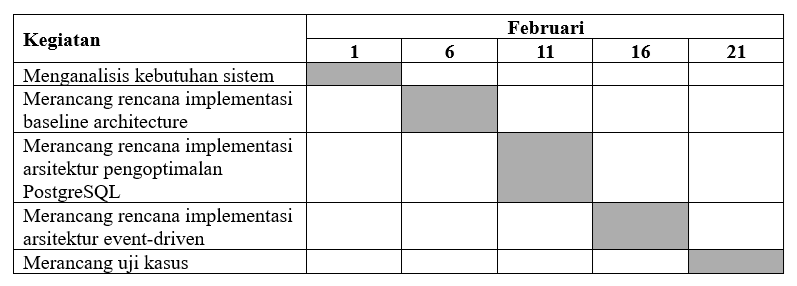
\includegraphics[width=1\textwidth]{resources/schedule/jadwal-1.png}
    \caption{Jadwal Pengerjaan Tugas Akhir Tahap Perencanaan}
    \label{fig:jadwal pelaksanaan perencanaan}
\end{figure}

\begin{figure}[htbp]
    \centering
    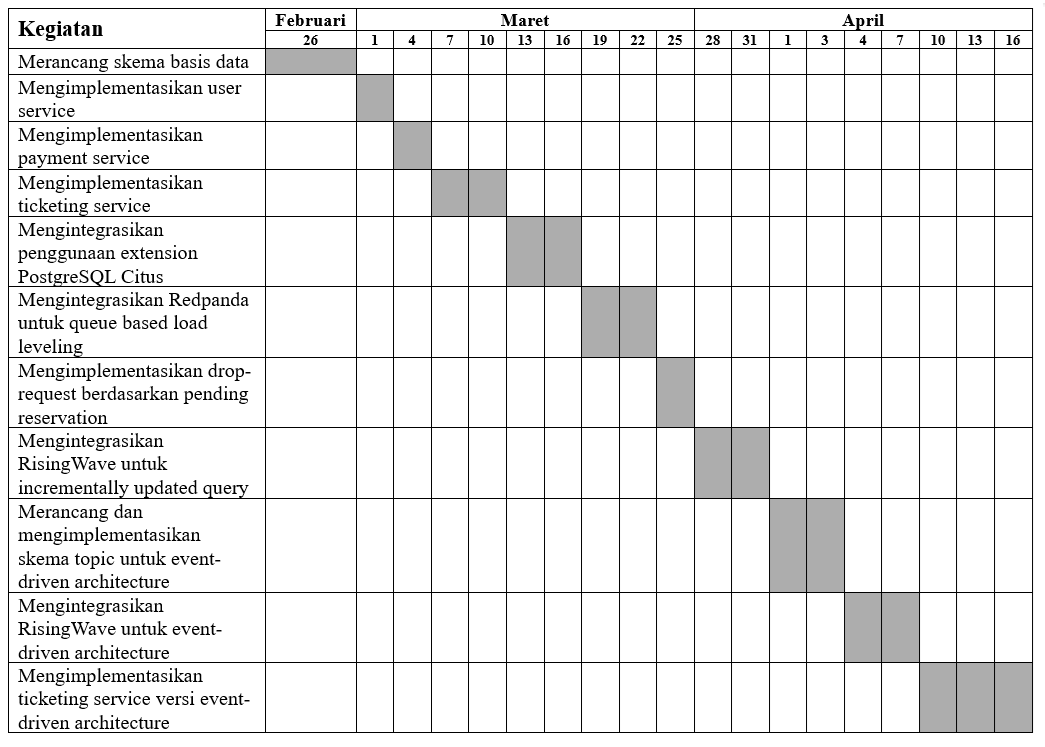
\includegraphics[width=1\textwidth]{resources/schedule/jadwal-2.png}
    \caption{Jadwal Pengerjaan Tugas Akhir Tahap Implementasi}
    \label{fig:jadwal pelaksanaan implementasi}
\end{figure}

\pagebreak

\begin{figure}[htbp]
    \centering
    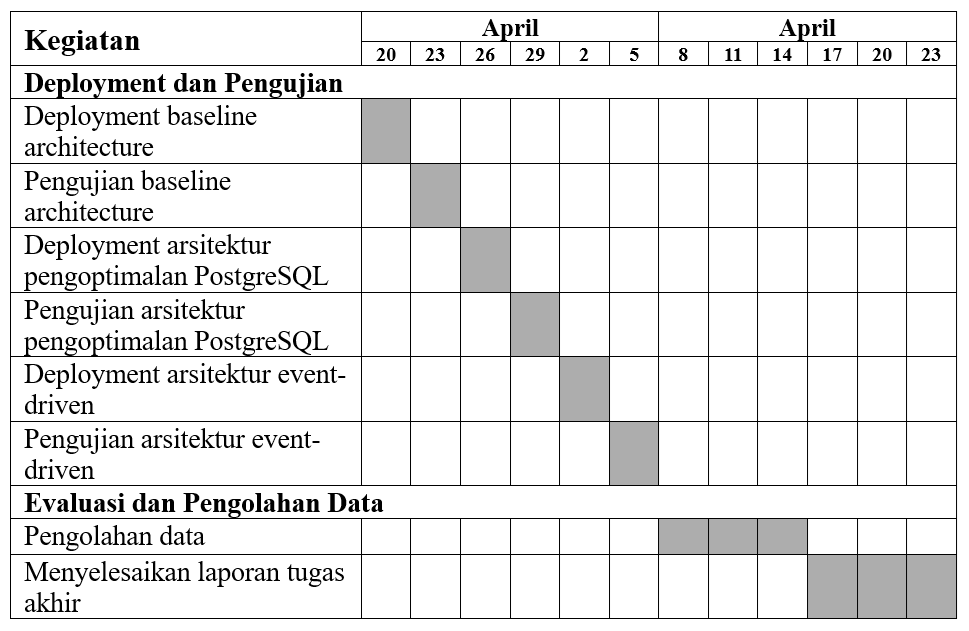
\includegraphics[width=1\textwidth]{resources/schedule/jadwal-3.png}
    \caption{Jadwal Pengerjaan Tugas Akhir Tahap Deployment dan Evaluasi}
    \label{fig:jadwal pelaksanaan deployment}
\end{figure}

Secara umum, proses pengerjaan terbagi menjadi empat tahap, yaitu:

\begin{enumerate}
    \item Tahap perencanaan yang meliputi penentuan kebutuhan, perancangan implementasi, dan perancangan uji kasus.
    \item Tahap implementasi yang meliputi implementasi untuk tiga arsitektur, yaitu arsitektur dasar acuan, arsitektur yang mengoptimalkan PostgreSQL, dan arsitektur \textit{event-driven}.
    \item Tahap \textit{deployment} dan pengujian setiap arsitektur.
    \item Tahap penyelesaian yang meliputi pengolahan data dan menyelesaikan sisa pekerjaan laporan tugas akhir.
\end{enumerate}

\chapter{Analisis Sistem}

\section{Komponen Sistem Tiket}

Berdasarkan studi yang sudah dibahas sebelumnya dan berdasarkan fokus yang ingin dibahas pada penelitian ini, berikut adalah komponen sistem yang menjadi bahasan dari penelitian ini:

\begin{enumerate}
    \item Layanan \textit{backend} utama yang memproses setiap permintaan yang berkaitan dengan pemesanan tiket.
    \item Layanan otentikasi.
    \item Layanan gerbang pembayaran. Layanan ini merupakan layanan eksternal dan cukup melakukan \textit{mocking service}.
    \item Terdapat satu basis data utama sebagai sumber kebenaran utama.
\end{enumerate}

Daftar acara dan ketersediaan awal tiket merupakan data yang diisi dari awal, sehingga fitur manajemen acara dan tiket tidak diimplementasikan. Detail lengkap komponen dan fitur sistem dijelaskan pada bagian lampiran.


\chapter{Arsitektur Solusi}

Komponen \textit{backend} utama bersifat \textit{stateless}, sehingga dapat di-\textit{scale} dengan meningkatkan jumlah \textit{instance}. Setiap arsitektur solusi memiliki dua layanan eksternal, yaitu layanan pengguna dan layanan gerbang pembayaran. Basis data merupakan komponen yang sulit di-\textit{scale} secara dinamis berdasarkan beban yang diterima. Biasanya, penskalaan secara vertikal merupakan opsi utama untuk meningkatkan \textit{throughput}.

\section{Arsitektur Dasar Acuan}

\begin{figure}[ht]
    \centering
    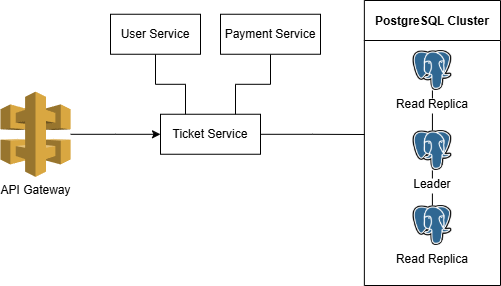
\includegraphics[width=0.8\textwidth]{resources/chapter-3/architecture-reference.png}
    \caption{Arsitektur Dasar Acuan}
    \label{fig:baseline-architecture}
\end{figure}

Arsitektur ini akan menjadi dasar acuan yang digunakan sebagai dasar perbandingan kinerja. Terdapat kluster PostgreSQL dengan konfigurasi satu node pemimpin dan sisanya node replika. Keberadaan replika memungkinkan peningkatan \textit{throughput} permintaan baca, tetapi tidak ada pengoptimalan untuk operasi tulis.

\section{Arsitektur yang Mengoptimalkan PostgreSQL}

Arsitektur ini mengoptimalkan sistem dengan pola CQRS. Tanggung jawab permintaan baca dilimpahkan kepada RisingWave. \textit{Streaming database} ini mengonsumsi \textit{CDC stream} dari kluster PostgreSQL, lalu memperbarui kueri secara inkremental. Penggunaan ekstensi Citus memungkinkan pembagian data berdasarkan baris dan \textit{multiple writer}. Selain itu, perintah pemesanan tiket (berupa \textit{command}/ \textit{event sourcing}) akan dimasukkan ke dalam antrean terlebih dahulu, lalu diproses secara bertahap. Redis digunakan untuk menyimpan \textit{uncommited data} dan menolak permintaan pemesanan lebih awal.

\begin{figure}[ht]
    \centering
    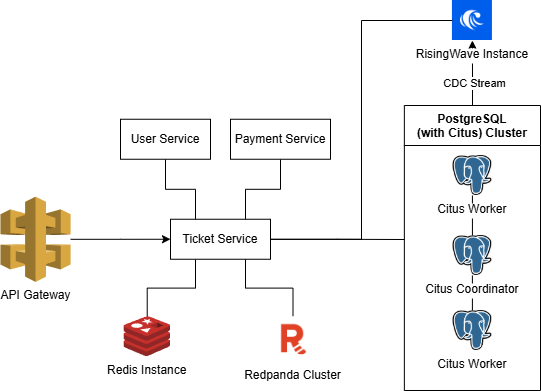
\includegraphics[width=0.8\textwidth]{resources/chapter-3/architecture-optimized.png}
    \caption{Arsitektur yang Mengoptimalkan PostgreSQL}
    \label{fig:optimized-architecture}
\end{figure}

Penggunaan ekstensi Citus memungkinkan penginkatan \textit{write throughput} tidak hanya dengan pendekatan \textit{scale up}, tetapi juga dengan pendekatan \textit{scale-out}. Redpanda dapat dibuat kluster dengan pemartisian data untuk meningkatkan \textit{throughput}. Redis dapat dikonfigurasikan dalam mode kluster untuk redundansi dan mode AOF untuk \textit{persistence}.

\section{Arsitektur \textit{Event-Driven}}

Arsitektur ini tidak menggunakan PostgreSQL sama sekali. Pada dasarnya, basis data relasional terdiri atas komponen \textit{storage} dan \textit{query processor}. Pada arsitektur ini, komponen \textit{storage} diganti menggunakan Redpanda dengan berbagai topik dan \textit{query processor} diganti dengan RisingWave. Meskipun begitu, pendekatan ini tidak memiliki dukungan \textit{transaction} selain \textit{transaction} pada Redpanda yang berupa \textit{push log all or nothing} pada beberapa topik sekaligus. Untuk itu, Redis digunakan untuk menyimpan \textit{dirty data} atau \textit{uncommited data} sehingga untuk mencegah \textit{double booking}.

\begin{figure}[ht]
    \centering
    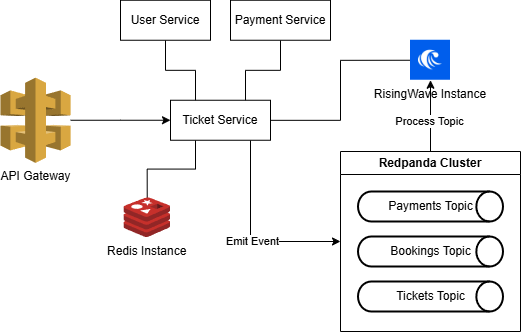
\includegraphics[width=0.8\textwidth]{resources/chapter-3/architecture-event-driven.png}
    \caption{Arsitektur \textit{Event-Driven}}
    \label{fig:solution-event-driven-architecture}
\end{figure}

Redpanda dapat dibuat kluster dengan pemartisian data untuk meningkatkan \textit{throughput}. Redis dapat dikonfigurasikan dalam mode kluster untuk redundansi dan mode AOF untuk \textit{persistence}. Selain itu, RisingWave merupakan \textit{streaming database} yang \textit{cloud-native} sehingga dapat di-\textit{scale out} dengan mudah untuk meningkatkan \textit{throughput}.



\chapter{Alternatif Solusi}

Bagian ini membahas alternatif pengoptimalan atau alternatif teknologi yang bisa menjadi opsi, tetapi tidak dipilih menjadi bagian dari solusi.

\section{Penggunaan \textit{Cache} dengan TTL Kecil}

Meski pada beban tinggi hasil kueri yang di-\textit{cache} akan selalu \textit{stale}, tetap ada durasi hidup (\textit{time to live}) \textit{cache} yang masih dapat diterima. Misalkan, waktu hidup \textit{cache} pembacaan ketersediaan adalah 100-200 milidetik. Rentang waktu ini masih memberikan \textit{data freshness} yang baik dan mampu meminimalkan jumlah kueri yang harus dilakukan sistem. Meskipun begitu, pendekatan ini harus dilakukan pada setiap arsitektur agar perbandingannya setara. Selain itu, pendekatan ini tidak sesuai dengan tujuan tugas akhir ini yang ingin mengoptimalkan operasi baca dan tetap memberikan hasil kueri yang \textit{fresh}.

\section{Alternatif Basis Data Terdistribusi}

Selain Citus, terdapat berbagai alternatif basis data terdistribusi lain, seperti Vitess, TiDB, YugabyteDB, dan CockroachDB. Berikut adalah perbandingan masing-masing solusi \parencite{citus,vitess,tiDB,yugabyte,cockroachDB}:

\begingroup
\footnotesize
\begin{longtable}{|p{0.14\textwidth}|p{0.14\textwidth}|p{0.14\textwidth}|p{0.14\textwidth}|p{0.14\textwidth}|p{0.14\textwidth}|}
    \caption{Perbandingan Antara Citus, Vitess, TiDB, YugabyteDB, dan CockroachDB}                                                                                                                                                                                                                    \\
    \hline
    \textbf{Aspek}            & \textbf{Citus}                                               & \textbf{Vitess}                                     & \textbf{TiDB}                                  & \textbf{YugabyteDB}                            & \textbf{CockroachDB}                           \\
    \hline
    \endfirsthead

    \multicolumn{6}{|c|}{\tablename\ \thetable\ -- \textit{Lanjutan dari halaman sebelumnya}}                                                                                                                                                                                                         \\
    \hline
    \textbf{Aspek}            & \textbf{Citus}                                               & \textbf{Vitess}                                     & \textbf{TiDB}                                  & \textbf{YugabyteDB}                            & \textbf{CockroachDB}                           \\
    \hline
    \endhead

    \hline
    \multicolumn{6}{|r|}{\textit{Dilanjutkan ke halaman berikutnya}}                                                                                                                                                                                                                                  \\
    \endfoot

    \hline
    \endlastfoot

    \hline
    Basis data yang mendasari & PostgreSQL                                                   & MySQL                                               & Dibuat dari awal                               & Dibuat dari awal                               & Dibuat dari awal                               \\
    \hline
    \hline
    Arsitektur                & \textit{Sharded Multi-Master with a Coordinator}             & \textit{Sharded Multi-Master with a Coordinator}    & \textit{Multi-Master with Shared Nothing}      & \textit{Multi-Master with Shared Nothing}      & \textit{Multi-Master with Shared Nothing}      \\
    \hline
    \hline
    Tipe                      & Ekstensi PostgreSQL                                          & Ekstensi MySQL                                      & Basis data terdistribusi dengan konsensus Raft & Basis data terdistribusi dengan konsensus Raft & Basis data terdistribusi dengan konsensus Raft \\
    \hline
    \hline
    Kompatibilitas SQL        & PostgreSQL                                                   & MySQL                                               & Kompatibel dengan MySQL 8.0                    & Kompatibel dengan PostgreSQL                   & Kompatibel dengan PostgreSQL                   \\
    \hline
    \hline
    Konsistensi               & Sama seperti PostgreSQL (konsisten dalam satu \textit{node}) & \textit{Eventual consistent} untuk operasi tertentu & ACID                                           & ACID                                           & ACID                                           \\
    \hline
    \hline
    Dukungan CDC              & Ada                                                          & Ada                                                 & Ada                                            & Ada                                            & Ada                                            \\
    \hline
    \hline
    Distribusi Data           & \textit{shard}                                               & \textit{shard}                                      & \textit{native distributed}                    & \textit{native distributed}                    & \textit{native distributed}                    \\
    \hline
\end{longtable}
\endgroup

Distribusi data yang \textit{natively distributed} masih sama-sama berupa \textit{sharding} data. Meskipun begitu, proses \textit{sharding} ini dilakukan secara otomatis dan tidak ditentukan oleh pengguna. Selain itu, suatu \textit{shard} dapat dipegang oleh beberapa \textit{node} sekaligus untuk mencapai \textit{redundancy} dan \textit{fault tolerance}.

Pada basis data terdistribusi seperti YugabyteDB, CockroachDB, dan TiDB, terdapat \textit{overhead} dalam koordinasi antarnode untuk operasi tulis, terlebih lagi setiap operasi tulis harus mencapai konsensus terlebih dahulu. Berbeda dengan basis data terdistribusi yang memakai koordinator seperti Citus dan Vitess, \textit{overhead} lebih kecil dan berada pada koordinator saja. Setelah koordinator menentukan node yang bertanggung jawab atas operasi tersebut, operasi langsung diarahkan kepada node yang berkaitan. Pendekatan konsensus memang memberikan konsistensi dan \textit{failover} yang lebih baik, tetapi terdapat \textit{tradeoff} berupa latensi yang lebih tinggi. Penggunaan basis data terdistribusi dengan konsensus akan lebih \textit{desirable} apabila melayani pengguna dalam beberapa \textit{region} yang berbeda. Meskipun begitu, penelitian ini berfokus pada pengoptimalan untuk satu \textit{region} yang sama.

Berdasarkan pembahasan di atas, terdapat dua pilihan yang tersisa, yaitu Vitess dan Citus. Citus dipilih agar basis \textit{database} yang digunakan sama, sehingga perbandingan antar arsitektur lebih disebabkan karena perbedaan arsitektur dan bukan karena perbedaan pengoptimalan pada basis data yang berbeda. Selain itu, basis data PostgreSQL merupakan basis data yang paling familiar dengan penulis dibandingan dengan MySQL.


\subsection{Penggunaan Solusi Basis Data \textit{Serverless}}

Penggunaan solusi serverless seperti Supabase, Neon, dan PlanetScale terbatas pada vendor tersebut. Solusi seperti ini memiliki banyak variabel yang tidak bisa dikontrol, terlebih lagi dari aspek biaya yang harus dikeluarkan untuk melakukan pengujian. Selain itu, terdapat batas atas penggunaan sumber daya yang diperbolehkan oleh setiap vendor. Batas atas ini baru bisa ditambah ketika melakukan \textit{subscription} dengan \textit{enterprise plan}. Oleh karena itu, penggunaan solusi \textit{serverless} tidak \textit{feasible} untuk dilakukan.

\subsection{Penggunaan Redis dan Alternatifnya}

Kenapa Redis dibandingkan dengan solusi KV lain

local dengan replikasi (redis), consensus based,

Konsensus: etcd, TiKV
Persistent: LevelDB by Google, RocksDB (fork of LevelDB by Facebook)
Fork redis: Valkey


\end{document}
